\documentclass[12pt]{article}
 
%\documentclass[fleqn]{article}
%\usepackage{palatino} 
%\usepackage{charter}
%\usepackage[T1]{fontenc}
%\usepackage{concmath} % pretty good
%\usepackage{cmbright}
%%%%%%%%%%%%%%%%%%%%%%%%%%%%%%%%%%%%%
\usepackage{/home/sci/weiliu/haldefs}
\usepackage{/home/sci/weiliu/notes}
\usepackage{/home/sci/weiliu/projects/lwdefs}
\usepackage{graphicx}
\usepackage{url}
\usepackage{textcomp}
%\usepackage[numbers]{natbib}
\usepackage{natbib}
\usepackage{subfig}
\usepackage{hyperref}
\usepackage{/home/sci/weiliu/packages/breakurl/breakurl}
%\usepackage{endfloat}
\usepackage{amsmath}
\usepackage{verbatim}
\usepackage{natbib}
\usepackage{algorithmic}
\usepackage{algorithm}

\hypersetup{
    bookmarks=true,         % show bookmarks bar?
    unicode=false,          % non-Latin characters in Acrobat’s bookmarks
    pdftoolbar=true,        % show Acrobat’s toolbar?
    pdfmenubar=true,        % show Acrobat’s menu?
    pdffitwindow=false,     % window fit to page when opened
    pdfstartview={FitH},    % fits the width of the page to the window
    pdftitle={Markov Random Field and fMRI},    % title
    pdfauthor={Author},     % author
    pdfsubject={Subject},   % subject of the document
    pdfcreator={Creator},   % creator of the document
    pdfproducer={Producer}, % producer of the document
    pdfkeywords={keywords}, % list of keywords
    pdfnewwindow=true,      % links in new window
    colorlinks= true,       % false: boxed links; true: colored links
    linkcolor=red,          % color of internal links
    citecolor=green,        % color of links to bibliography
    filecolor=magenta,      % color of file links
    urlcolor=cyan           % color of external links
}



\begin{document}
\title{Notes: Markov Random Fields and fMRI}
\author{Wei Liu}
\maketitle
\tableofcontents
%\newpage
\section{Ising Model}
In this section I did test on Ising model. Following example 1 in \cite{perez_markov_1998}, I sampled the prior the distribution of hidden variable $\vec x$ on a $255\times 255$ binary images. Results at fig. \ref{fig1}.

Also apply Ising prior on a image denoising application: 1) Get a original image and apply 10\% noise. 2) denoise with no spatial prior, with little and much prior. Results at fig. \ref{fig2}.

\begin{figure}[hbt]
\centering
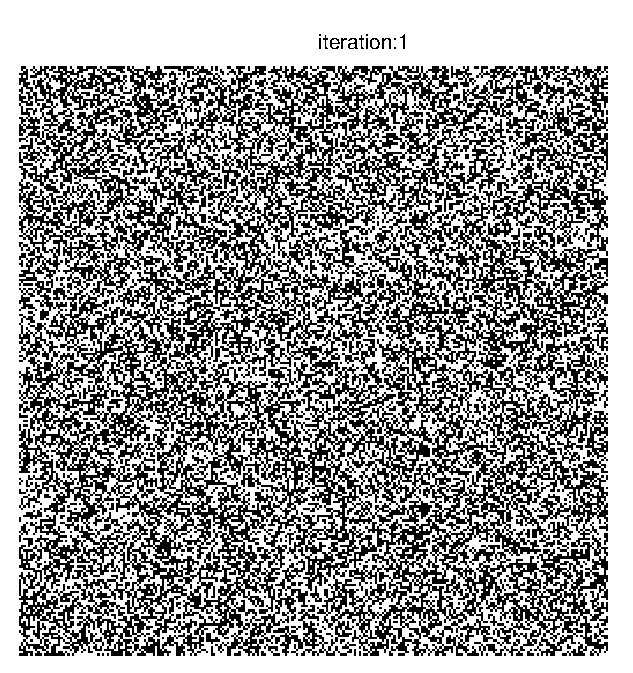
\includegraphics[width = 0.24\textwidth]{figures/Ising1.eps} 
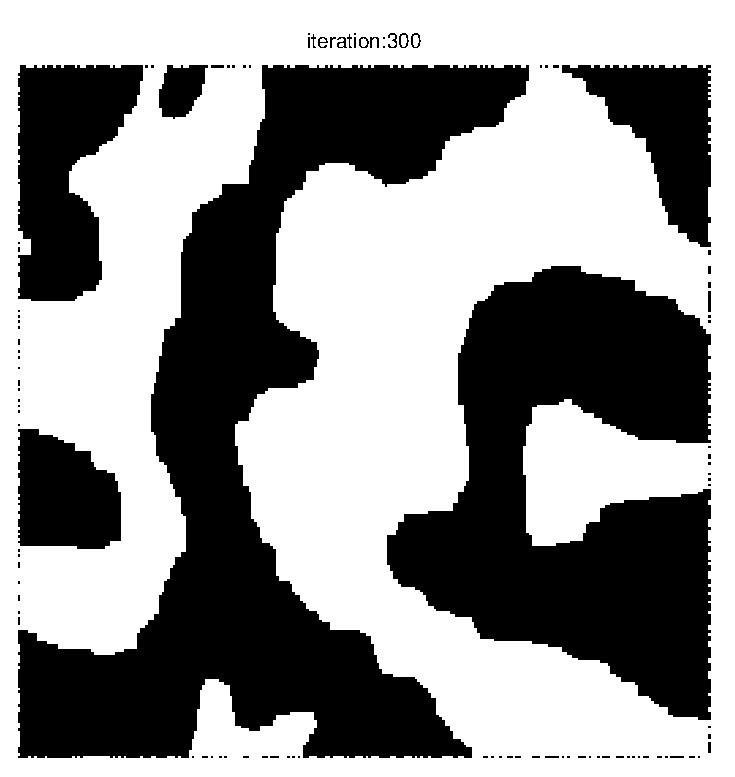
\includegraphics[width = 0.24\textwidth]{figures/Ising300.eps}
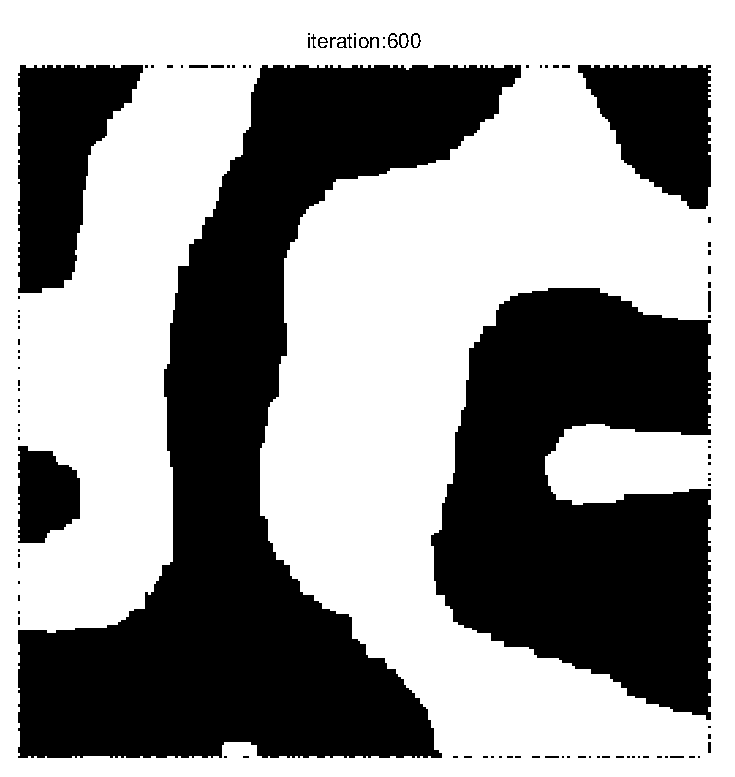
\includegraphics[width = 0.24\textwidth]{figures/Ising600.eps}
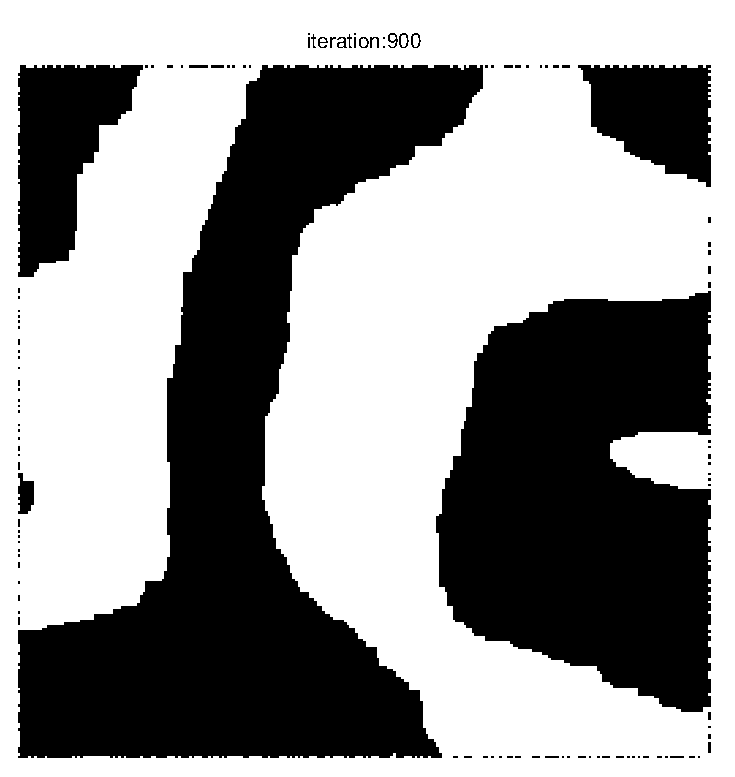
\includegraphics[width = 0.24\textwidth]{figures/Ising900.eps}

\caption{Initial image with uniform random -1 an +1. Update eqch pixel in sequence by the conditional probability. And repeat this many 1000 times. Here is the iteration for 1st time, 300, 600 and 900.}
\label{fig1}
\end{figure}

\begin{figure}[hbt]
\centering
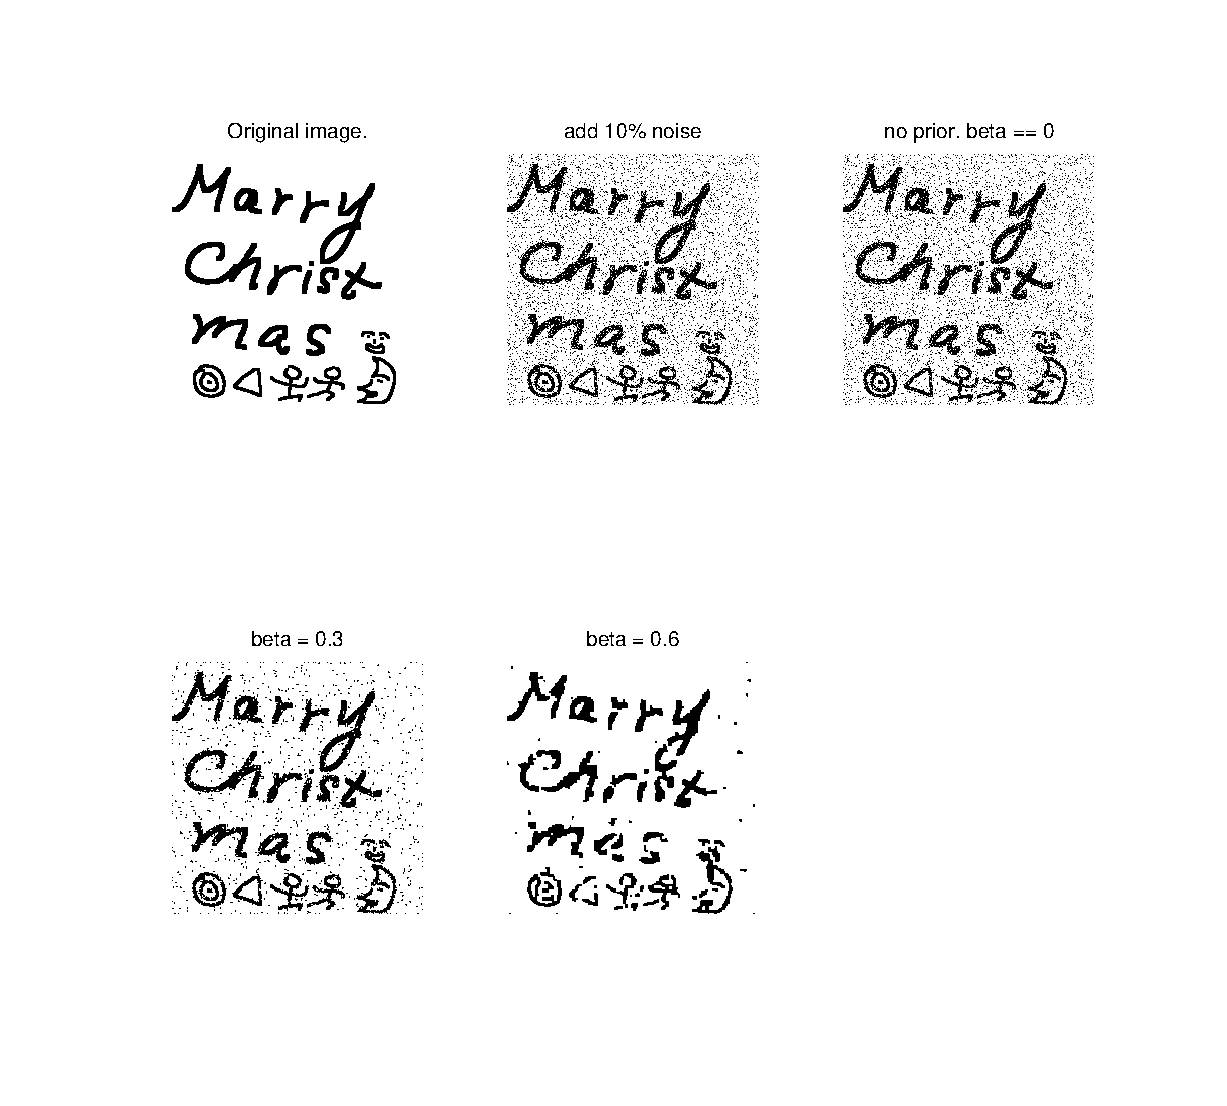
\includegraphics[width = 0.8\textwidth]{MarryChristmas.eps}
\caption{$\beta$ controls how strong the prior is, compared to the conditional likelihood $P(\vec y |\vec x)$. Greater $\beta$ means the energy function prefer prior rather than data.}
\label{fig2}
\end{figure}
\subsection{Generate Ising model by Gibbs Sampling}
In this test I want to generate a Ising model using Gibbs sampling. The possible gray level for each data point is {-1, 1} and I'm going to use Gibbs sampling method to generate the prior image in Gibbs distribution.

The Gibbs distribution is defined by
\begin{equation}
P(\vec x) = \frac{1}{\mat Z}\exp\{-\mat U(x)\}
\end{equation}
The conditional probability of data point $x_s$ is given by
\begin{align}
p(x_s | x_{i\neq s}) &= \frac{\frac{1}{\mat Z}\exp\{-\sum_{C\in \mathcal{C}}V_C (\vec x_C)\}}{\sum_{x_s = 0}^{M-1}\frac{1}{\mat Z}\exp\{-\sum_{C\in \mathcal{C}}V_C (\vec x_C)\}} \\
 &= \frac{\frac{1}{\mat Z}\exp\{-\sum_{C:s\in C}V_C (\vec x_C)\}}{\sum_{x_s = 0}^{M-1}\frac{1}{\mat Z}\exp\{-\sum_{C: s\in C}V_C (\vec x_C)\}} \\
&= \frac{\exp\{-\sum_{C:s\in C}V_C (\vec x_C)\}}{\sum_{x_s = 0}^{M-1}\exp\{-\sum_{C: s\in C}V_C (\vec x_C)\}} \\
\end{align}

So we only need to compute the potential function for those $V_C$ that include $x_s$. Define $V_C$ as 
\begin{equation}
V_C(x_i, x_j) = \left \{
\begin{array}{l l}
1 \quad \mbox{when } x_i \neq x_j\\
0 \quad \mbox{when } x_i = x_j\\
\end{array} \right .
\end{equation}
We don not need to have bigger potential function value for those $|x_i - x_j|$ is large, because $x_i$ and $x_j$ as labeling, should make no difference on potential as long as they are different.

The difference between Gibbs sampling and Metroplis Sampling is, Gibbs sampling need to compute conditional probability of $p(x_s | x_{i\neq s})$, which take much computation when th possible value of $x_s$ is large. For binary image like Ising model, possible value of $x_s$ is just two, and Gibbs Sampling has no problem computing that.

\begin{figure}
\centering
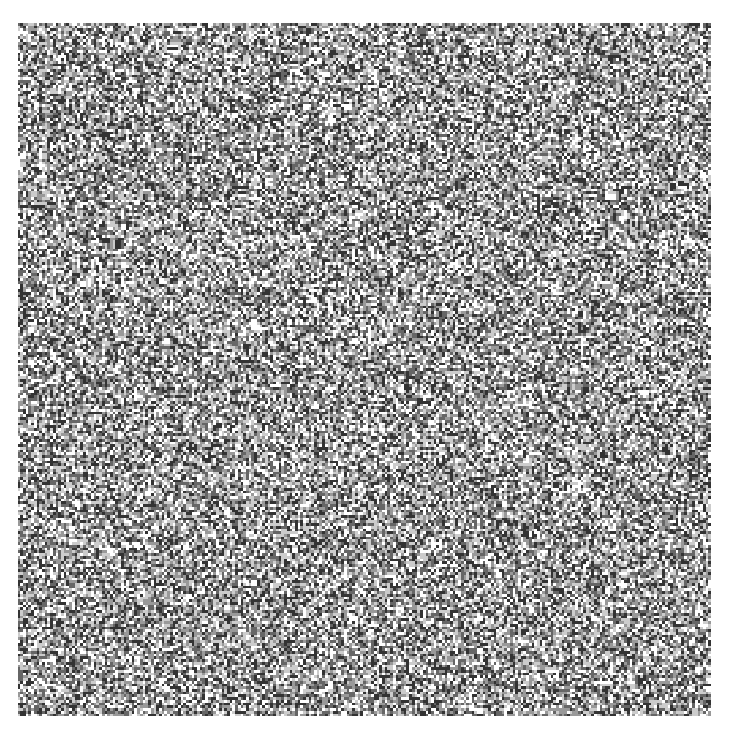
\includegraphics[width = 0.24\textwidth]{figures/Gibbs01.eps} 
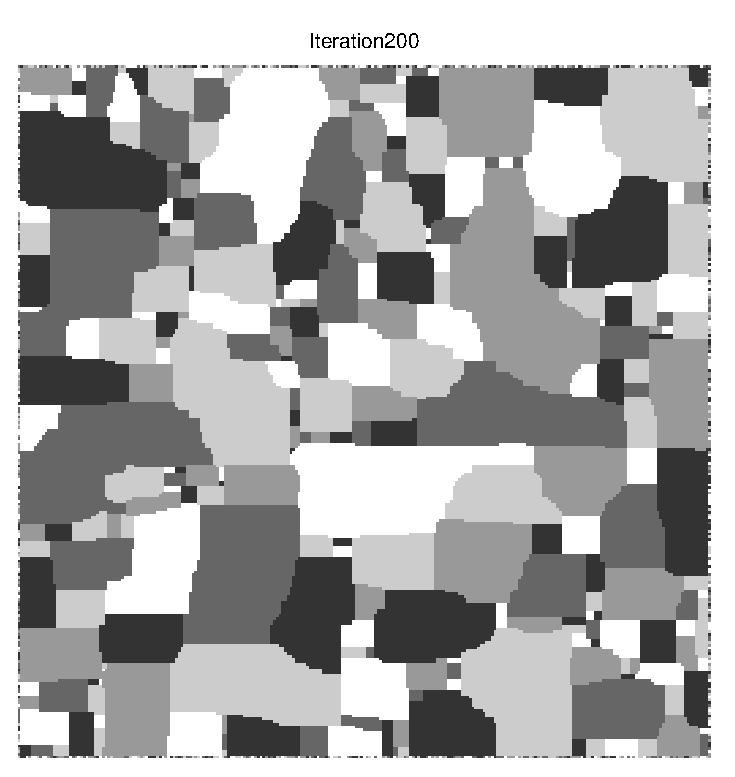
\includegraphics[width = 0.24\textwidth]{figures/Gibbs200.eps} 
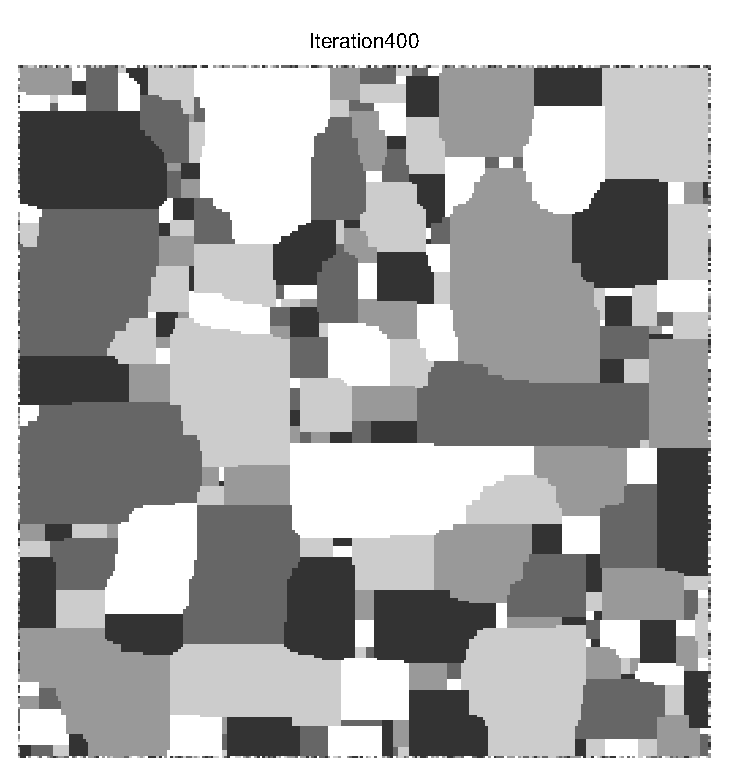
\includegraphics[width = 0.24\textwidth]{figures/Gibbs400.eps} 
\caption{Gibbs sampling to generate Gibbs distribution. Upper-left is the random generated  original 255x255 image with five gray level intensity. Upper-right is after 300 iterations of Gibbs sampling, with each iteration having raster scan through each pixel. Lower images are iterations 400 and 600 times.}
\label{Gibbs01}
\end{figure}

Figure \ref{Gibbs01} is the simulation result


Question: When the possible gray level is more than two, how do I generate them in Gibbs distribution (suppose I can compute the probability of each possible value, i.e. $P(\vec x = x_0)$, $P(\vec x = x_1)$, ... (Solved)
\subsection{Jan 19 Generate 1D fMRI image and compute posterior distribution}
\begin{figure}
\centering
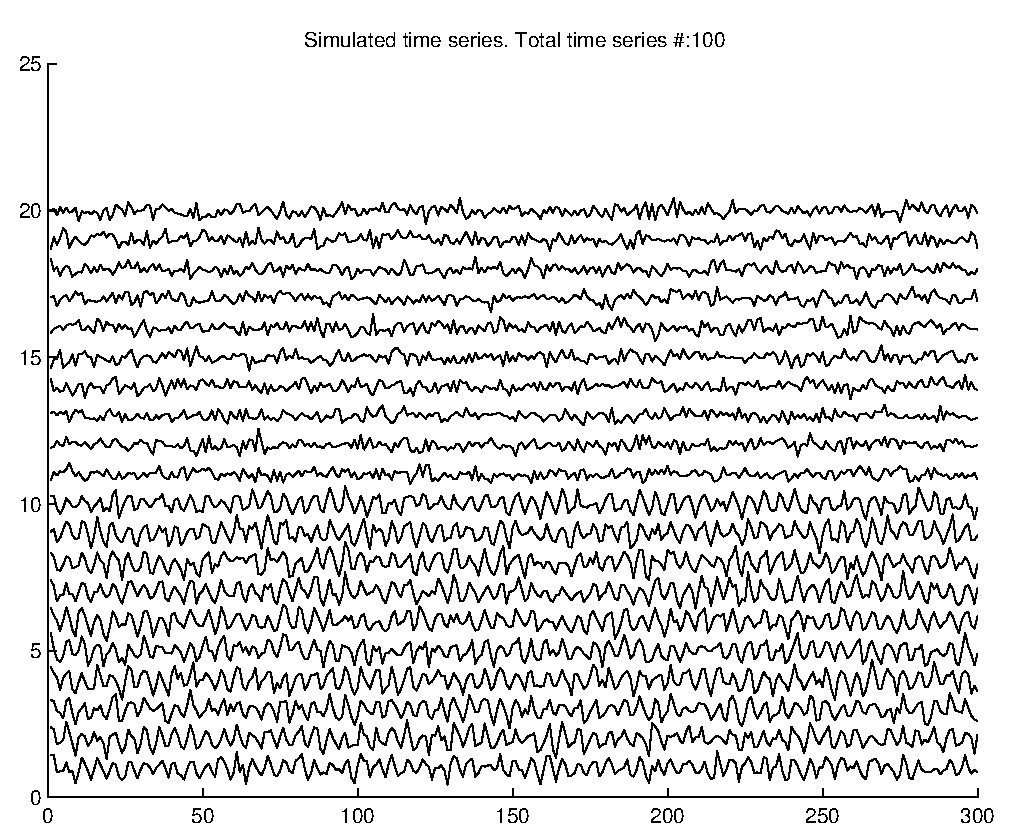
\includegraphics[width = 0.95\textwidth]{1DTimeSeries.eps} 
\caption{Generate N time series. Some are sin wave + Gaussian noise, others are purely Gaussian noise. Visualize them in a single plot by shifting the mean of each time series according to its label (from 1 to N)}
\label{1D}
\end{figure}

\begin{figure}
\centering
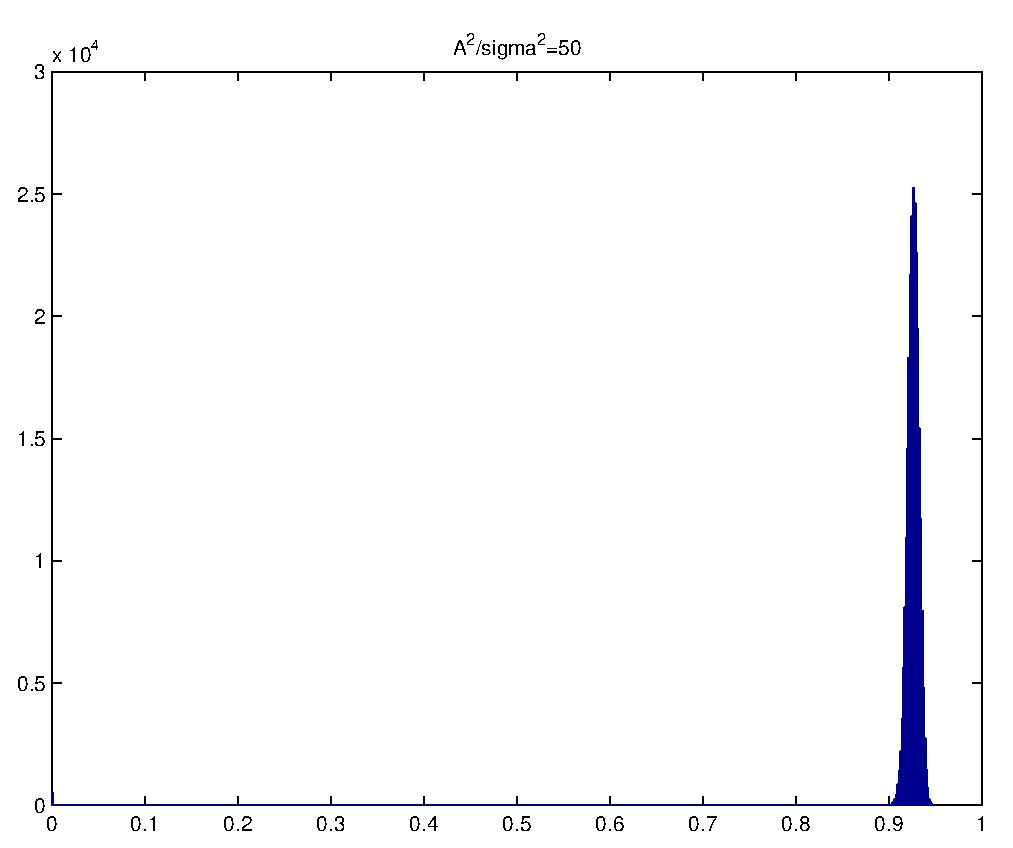
\includegraphics[width = 0.24\textwidth]{figures/empriLL50.eps} 
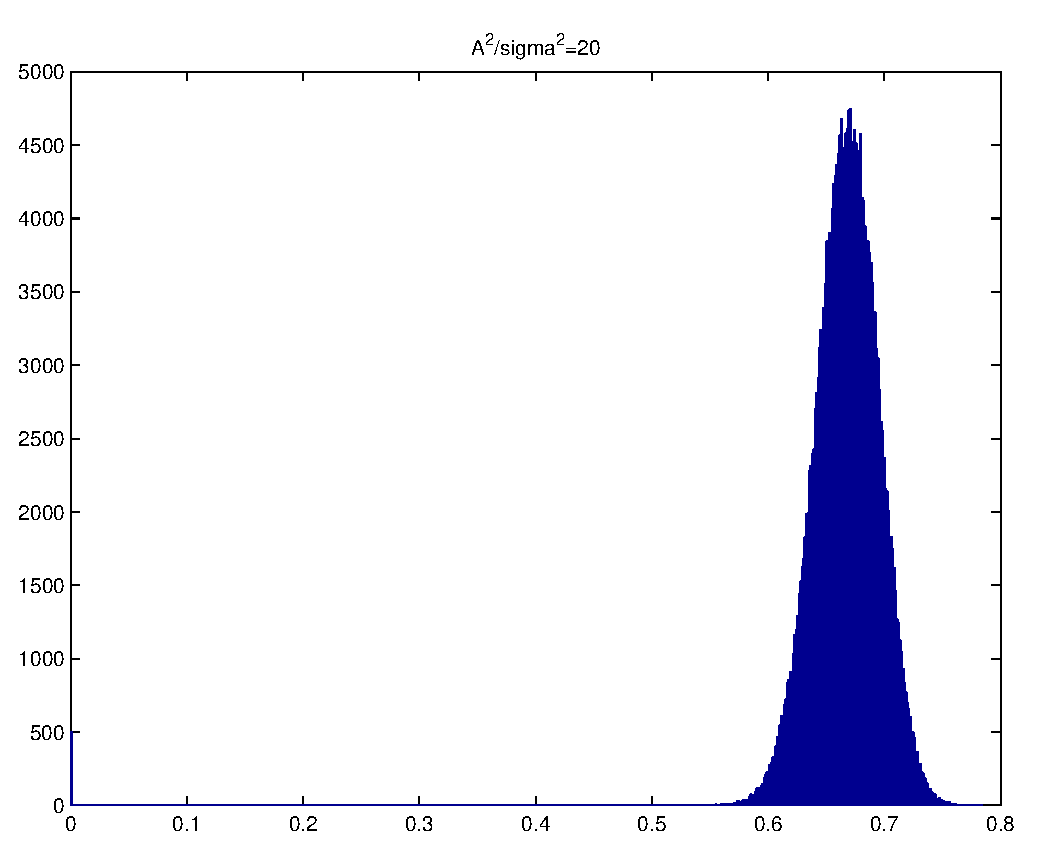
\includegraphics[width = 0.24\textwidth]{figures/empriLL20.eps} 
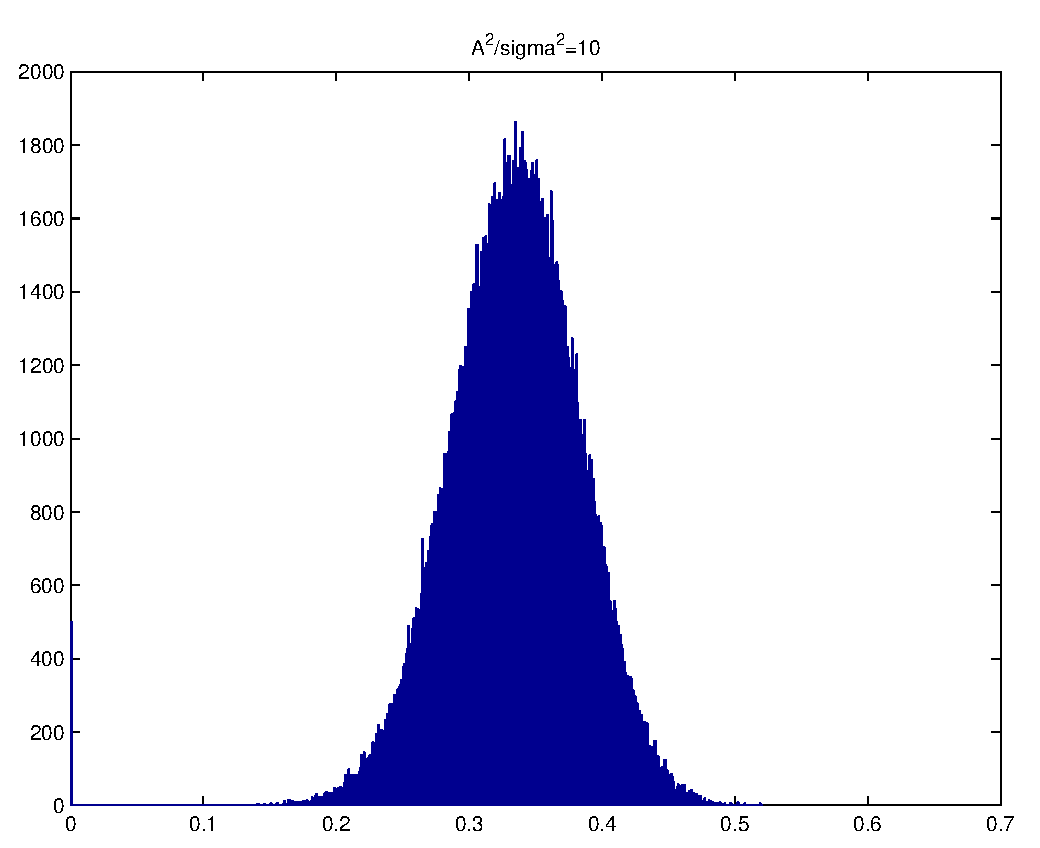
\includegraphics[width = 0.24\textwidth]{figures/empriLL10.eps} 
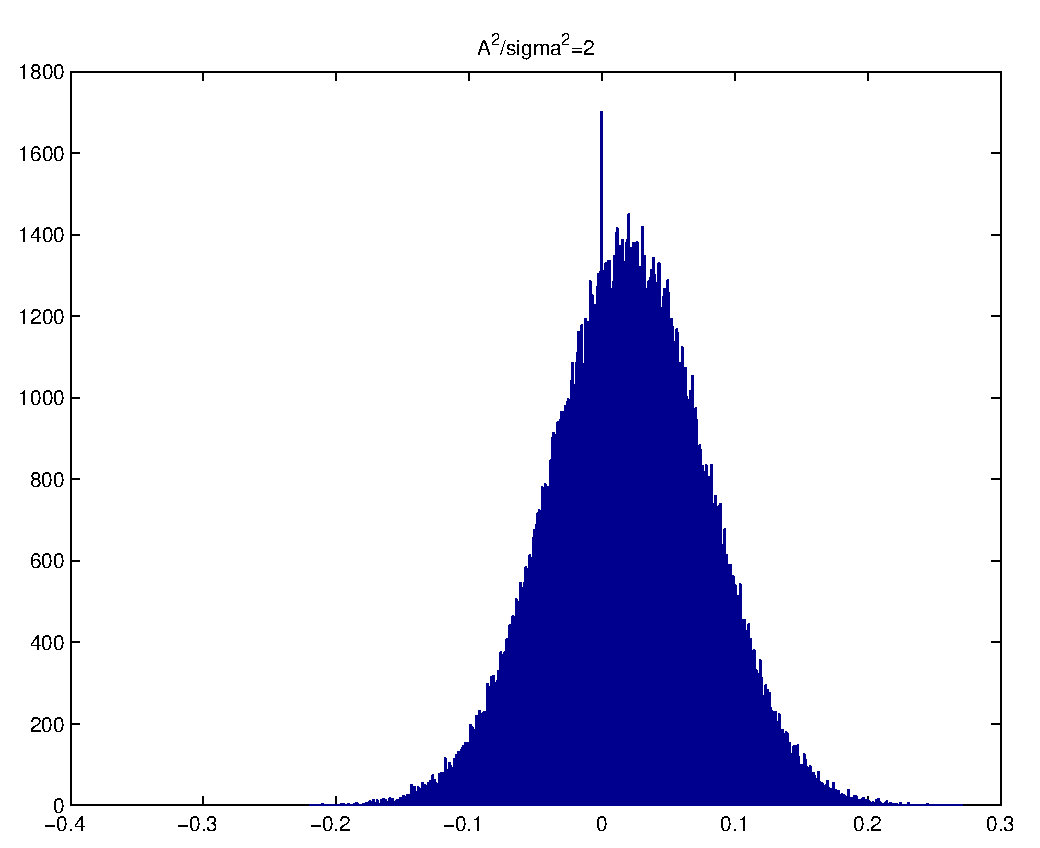
\includegraphics[width = 0.24\textwidth]{figures/empriLL2.eps} \\
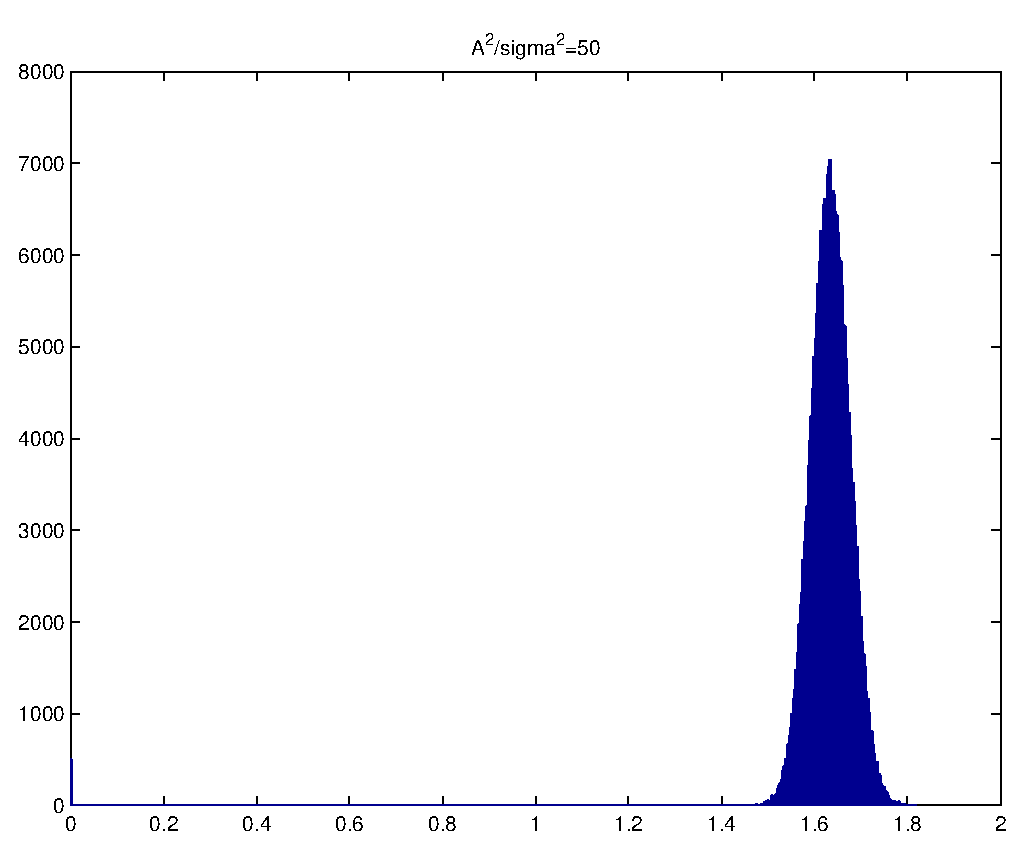
\includegraphics[width = 0.24\textwidth]{figures/empriLL50z.eps} 
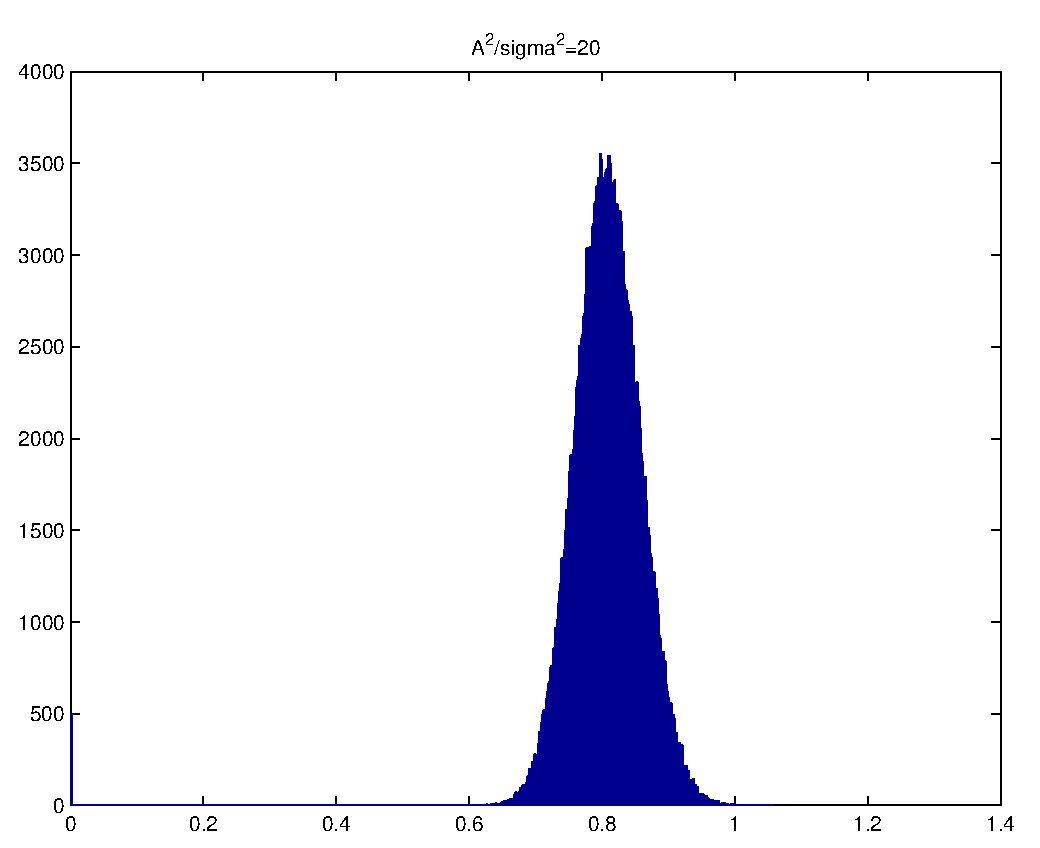
\includegraphics[width = 0.24\textwidth]{figures/empriLL20z.eps} 
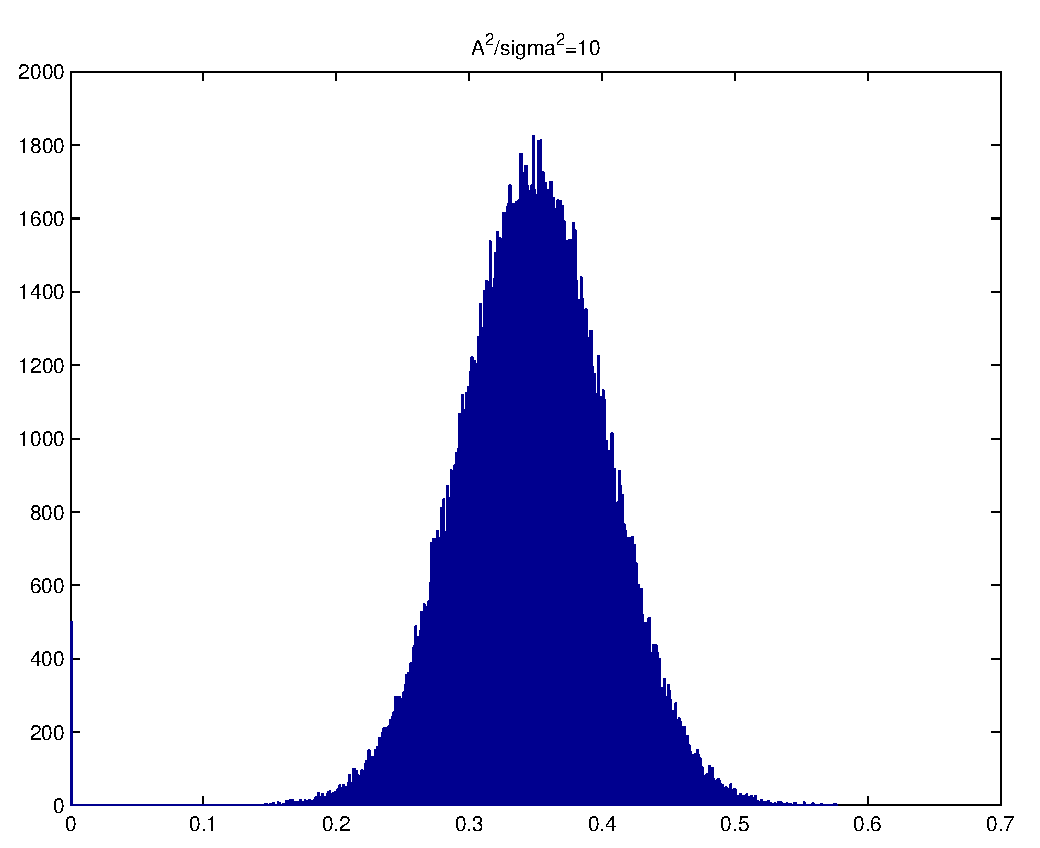
\includegraphics[width = 0.24\textwidth]{figures/empriLL10z.eps} 
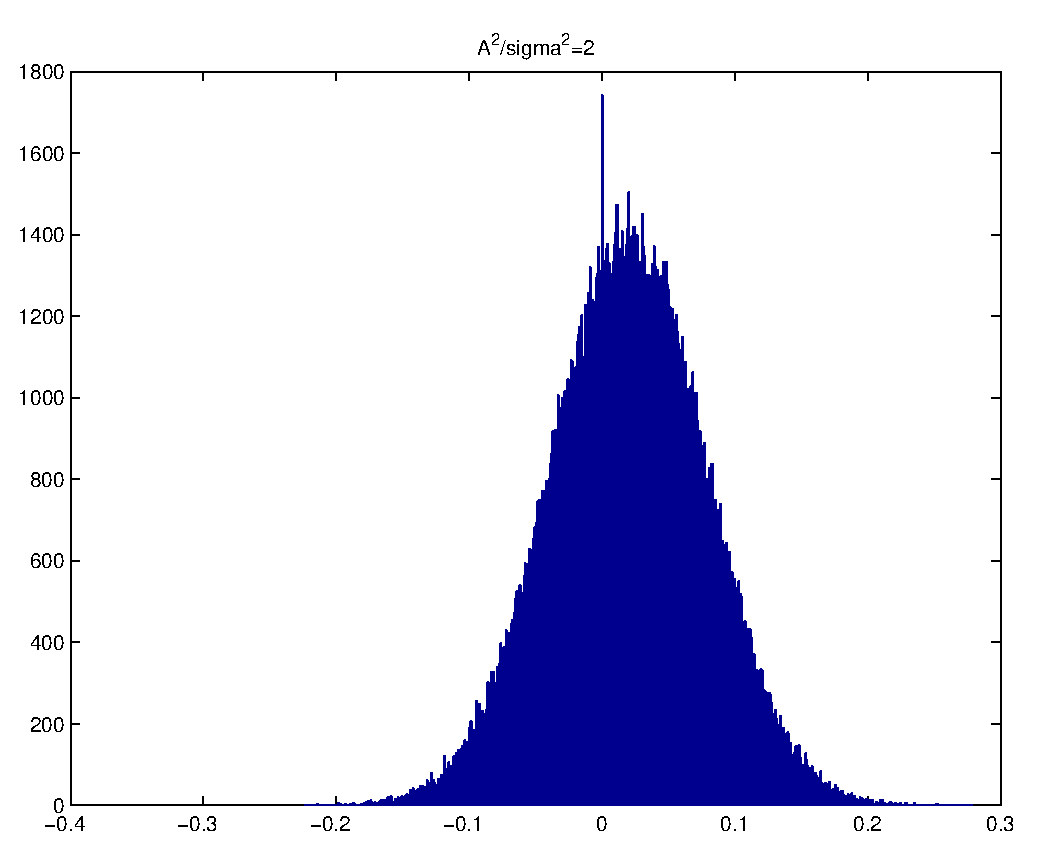
\includegraphics[width = 0.24\textwidth]{figures/empriLL2z.eps} 
\caption{The empirical distribution of the correlation between pair of $x_i$ and $x_j$ given they are 'connected'. To make them connected I generate all x from same sin wave plus independent Gaussian noise with different variance. A is amplitude of sin wave, and $\sigma$ is standard deviation of the Gaussian noise. I define $A^2/\sigma^2$ as the signal-to-noise ratio. On the bottom row is the empirical distribution of the z after Fisher Transformation. From Wikipeidia, Fisher transformation z is approximately normal only when 1) $x_i$ and $x_j$ are normal distribution, and 2) $x_i$ and $x_j$ are independent. Both conditions are not true in our case. But I just do the transformation and see the z's distribution.}
\label{1D}
\end{figure}

Two questions about Fisher transformation: 1) When data point $x$ and $y$ are not independent, is $z = 0.5*\ln (\rho+1/\rho-1)$ still approximately Gaussian distribution? 2) No matter if data point $x$ and $y$ are independent, to assume $z$ is approximately Gaussian, we must make sure sample correlation $r_i$ are independent over all $i = 1,...,N$. But in MRF, connectivity $c_i$is not independent, i.e. $P(c_i|c_{j\neq i} \neq p(c_i)$. Does this mean the p(r|c) is not independent?

I think even $c$ is not independent, $r_i$ is still independent given $c_i$, by the theory of conditional independence. That is, $p(r_1, r_2| c_1, c_2) = p(r_1|c_1)\cdot p(r_2|c_2)$. 

Now to compute posterior probability of connectivity $c$, I can use Gibbs Sampling(or Simulated Annealing) and EM algorithm to iteratively compute the posterior probability and model parameter. Here is the notations:
\begin{itemize}
\item $S$ is the set of lattice points.
\item $s$ is a lattice point, $s \in S $.
\item $X_s$ is the value of X at s. In our case, $X_s$ is the connectivity between two voxels. $X_s \in \{-1, 1\}$. It is also the latent variable we're interested in.
\item $\partial s$ is neighboring points of $s$.
\item $x_c$ is the value of $X$ at the points in clique $c$.
\item $V_c(x_c)$ is potential function.
\item $Y_s$ is correlation at site $s$. $y_s$ is sample correlation between two voxels. 
%\item $p(c)$ is prior distribution. By MRF theory, $p(c)$ is Gibbs distribution.
%\item $\rho$ is population correlation. 
%\item $r$ is sample correlation, as an estimation of $\rho$.
%\item $p(r|c)$ is likelihood function. In term of MRF, it is emission function.
%\item $p(c|r)$ is posterior function, the one we're interested. 
\end{itemize}

We do not know the likelihood. There are two options: 1) Assume a data model used to generate $Y$. For example, we can assume two data point $\tilde d_i$ and $\tilde d_j$ and assume they are clear signal without any noise. Further assume they are perfectly correlated. Then generate two noised signal $d_i = \tilde d_i + N_i$ and $d_j = \tilde d_j + N_j$. $N_i$ and $N_j$ are additive Gaussian noise term with zero mean. Then we try to compute probability $corr(d_i, d_j)$ given the fact $\tilde d_i$ and $\tilde d_j$ are perfectly correlated. 2) We can generate some sample correlation $y_s$ from data points $d_i$ and $d_j$ given $\tilde d_i$ and $\tilde d_j$ have correlation one. This can be see as Monte Carlo method. From figure \ref{1D} we see even $d_i$ and $d_j$ are correlated, their sample correlations are approximately Gaussian distribution after Fisher Transformation.

So I assume the likelihood function $p(y_s|x_s = 1)$ is Gaussian with unknown $\mu_1$ and $\sigma_1^2$. We already know $p(y_s|x_s=0)$ is Gaussian with know $\mu_0 = 0$. To compute both the posterior $p(X|Y)$ and the parameters $\mu_1$ and $\sigma_1^2$ and $\sigma_0^2$ try to use EM algorithm as below:
\begin{algorithm}                 
\caption{EM-Annealing}         
\label{alg1}                   
\begin{algorithmic}            
\REQUIRE Sample correlation matrix $\mat Y$ with $y_s$ the sample correlation between voxel $i$ and $j$.
%\ENSURE $y = x^n$
\STATE Init posterior matrix $\mat X: x_s = \argmax \ln p(Y_s | x_s; \theta) $.

\WHILE{Some Condition}
\STATE \textbf{E step: }

(1) Based on the current parameters $\vec \theta = \{\mu_0, \mu_1, \sigma_0^2, \sigma_1^2, \beta\}$, compute the posterior probability as
\begin{equation}
p(X_s | Y_s = y_s) = \frac{p(X_s)\cdot p(Y_s = y_s | X_s, \vec \theta)}{p(Y_s = y_s | \vec \theta)} \label{eq1z}
\end{equation}
(2) Repeatedly Do Gibbs Sampling from \eqref{eq1z} until the field stabilize.

(3) Based on current value of $X_s$, iteratively compute the mean field
\begin{align}
p(X_s | < X_{\partial s}>) &= \frac{1}{Z_s} \exp\{-\beta U_s(X_s | <X_{\partial s}>\}\\
Z_s &= \sum_{X_s\in \{-1, 1\}}^{}\exp\{-\beta U_s(X_s | <X_{\partial s}>\}\\
<X_s> &= \sum_{X_s\in \{-1, 1\}}^{} X_s \cdot p(X_s | <X_{\partial s}>)
\end{align}
\STATE \textbf{M step: }

(4) With compute data $\{X, Y\}$, estimate $\beta$ by maximizing log-likelihood of posterior probability of $X$. Because likelihood $p(Y | X)$ does not depend on $\beta$, we only maximize prior $p(X)$, which is Gibbs distribution. We use Newton's method. (To be added)

(5) Estimate $\mu$ and $\sigma^2$ by maximizing conditional log-likelihood $p(Y | <X>)$. (To be added)
\ENDWHILE
\end{algorithmic}
\end{algorithm}

\textbf{Issue 1: }If there is negative correlation in the sample correlation, we need to model this component. We need to look at the histogram of sample correlation on real data, and see if there is much negative correlation. If there is, we need to add another state for connectivity, i.e. $c_{ij} = -1$ to model this component.

\textbf{Issue 2: }Need to assume the latent variable 'connectivity' is continuous in $[0, 1]$, instead of the discrete $\{0, +1\}$ for current model. 

\textbf{Issue 3: } How to change the temperature $T$ in annealing of E step? Two option 1) Keep $T$ unchanged in each iteration of EM. That is, $T$ is constant over the annealing. Over all E step, T decreases.  2) $T$ decrease over annealing in a single E step of EM. At the beginning of annealing of each E step, $T$ begins with a high value. 

\textbf{Issue 4: } In terms of `neighbors', we can define two types of neighbors: `local neighbors' and `remote neighbors'. Local neighbors is those data points spatially close to the data we're interested in. Remote neighbors are data that are not necessarily spatially close, but are close according to some defined features (like DTI connection). And we can use Suyash's theory: to know current pixel, we not only look at its local neighbors (like MRF), and also look at its remote neighbors.

\textbf{issue 5: } When applying prior, we have to be careful not to smooth `edges'. When we find edges, we should not assume the pixels on two sides of edges are neighbors (either local neighbors, or remote neighbors). the edges are not given, but to be computed in the iteration algorithm. (need to study this later)

\textbf{Issue 5:} If we can assume the posterior distribution is also a Gibbs distribution,  we can use annealing on posterior Gibbs, instead of only on prior. In this method, there is an additional parameter $\alpha$ to control the weights between the prior energy and likelihood energy (update: From Gelman's paper, seems there is no such $\alpha$, posterior energy just sum of prior and likelihood energy, not weighted sum.)

To prove the posterior distribution $p(c_n | r_n)$ is also Gibbs distribution, we just need to prove it is Markov Random Field. Assume $\partial c$ is the neighbors of $c_n$, and $\tilde C$ is the set of other nodes that does not include $c_n$ and $\partial c$. We need to prove 
\begin{align}
p(c_n | r_n, \partial c, \tilde C) &= p(c_n | r_n, \partial c)
\end{align}
while we know that 
\begin{align}
p(c) &\sim \mbox{Gibbs}, \qquad  p(c_n|\partial c_n, \tilde C) = p(c_n | \partial c_n)\\
p(r_n | c_n ) &= \cN(\mu, \sigma^2) \\
\end{align}

Now rewrite the posterior as
\begin{align}
p(c_n | r_n, \partial c_n, \tilde C) &= \frac{p(c_n) \cdot p(r_n, \partial c_n, \tilde C | c_n)}{p(r_n, \partial c, \tilde C)} \\
&= \frac{p(c_n) \cdot p(r_n \ c_n) \cdot p(\partial c_n, \tilde C| c_n)}{p(r_n) \cdot p(\partial c_n, \tilde C)}\\
&= \frac{p(r_n | c_n)}{p(r_n)}\cdot p(c_n | \partial c_n, \tilde C)\\
&= \frac{p(r_n | c_n)}{p(r_n)}\cdot p(c_n | \partial c_n) \label{eq1}
\end{align}

\begin{align}
p(c_n | \partial c_n) &= \frac{p(c_n) p(r_n, \partial c_n| c_n)}{p(r_n, \partial c_n)}\\
&= \frac{p(c_n) \cdot p(\partial c_n| c_n) \cdot p(r_n | c_n)}{p(r_n) \cdot p(\partial c_n)}\\
&= \frac{p(c_n, \partial c_n) \cdot p(r_n | c_n)}{p(r_n) \cdot p(\partial c_n)} \label{eq2}
\end{align}

We see \eqref{eq1} and \eqref{eq2} are equal, so we prove the posterior is also Gibbs.

\textbf{SNR of functional MRI data: } It is better to view fMRI data as time series and define signal-to-noise ratio from signal processing standpoint, i.e. 
\begin{equation*}
SNR = \frac{P_{sig}}{P_{no}} = \(\frac{A_{sig}}{A_{No}}\)^2
\end{equation*}

According to this definition, the 'auditory' data set has SNR closet to 1.0. This is better than $SNR = A_{sig}/ \sigma_{no}^2$. If $SNR = A_{sig}/ \sigma_{no}^2 = 1$, we have at least one time point among 100 time point that can reach $3\sigma = 3$, and by signal processing definition, the SNR would be 1/3.

\section{New Reading on Functional Connectivity}
\section{Apr 6 Meeting}
-- Add one clique potential energy function.\\
-- Add edge process to preserved edges when annealing.\\
-- When estimating parameters, again we can use simulated annealing (or Metroplis-Hasting) to find the global maximum of the psudo-likelihood with respect to parameters.\\
-- Change 26 neighbors back to 12 neighbors.
-- 

\section{Apr 20}
\textbf{Prerocessing: } The processing takes following steps:
\begin{itemize}

\item Slice timing correction. After this step, I get image
  \texttt{rawfmriS}.
  \item motion correction with middle volume as reference. After this
    step I get motion corrected image \texttt{rawfmriSC}. 
  \item Remove skull and scalp of t1, t2 and middle volume of fmri
    image by fsl tool \textsf{bet}, and get results in \texttt{t1B}
    and \text{t2B}.
  \item Register scalp-removed \texttt{t2B} to \texttt{t1B}, and get
    \texttt{t21}. 
  \item Segmentation of t1B using FSL tool
    \textsf{fast}, get gray matter mask image \texttt{t1B\_pve\_1}.

  \item Register fmri (scalp removed middle volume \texttt{midB}) to \texttt{t21},
    and get transformation matrix \texttt{mid\_t2B.mat}.

  \item Invere the matrix \texttt{mid\_t2B.mat}, and get trans. matrix
    \texttt{t2B\_mid}.
  \item  Use the intervse matrix in previous to register gray matter mask image to middle fmri image, and get \texttt{mask}.
  \item Now register t1B (scalp removed t1 image) to MNI altas, only to get the transformation matrix.
  \item concatenate two transforms. \texttt{fmri}$\rightarrow$ \texttt{t21}, and \texttt{t1} $\rightarrow$ \texttt{MNI}. The goal is to get trasformation of \texttt{fmri} $\rightarrow$ \texttt{MNI}.

\item Given the coordinates in MNI space and the transform matrix in previous step, use FSL tool \textsf{std2imgcoord} to find the coordinates(voxel) in fmri image. The reason of doing this step is, for fMRI image of different subject, we do not have to mannually pick CSF or white matter voxel. We just choose a coordinate of CSF/WM in standard MNI space, and the script automatically find the voxels in fMRI space. 
\end{itemize}

After above steps, the \texttt{mask} image looks better than what I got from \texttt{t2} image. one thing nee mention is when removing scalp and skull from \texttt{t2}, the results is not good. But since we only use scalp remove \texttt{t2} for registration between \texttt{t1} and \texttt{fMRI}, this does not matter much. 

\textbf{Number of Voxels in gray matter: } When thresholding \texttt{t1} mask image at $0.5$, the number of voxels in gray matter is $15,325$. Set threshold at $0.4$ give the number $18,654$. 

\section{GPUSampling code change memo}
\begin{align*}
  V_c(x_i, x_j) &= -\beta x_i x_j \\
  U &= \sum_C V_c \\
  p(\vec x) &= \frac{1}{Z}\exp\{-U(\vec x)\} \\
  p(x_i) &= \frac{1}{Z_i}\exp\{ \sum \beta x_i x_j\} = \frac{1}{Z_i}\exp\{ \beta \sum x_i x_j\} \\
  p(x_i | \cdot) &= \frac{\exp\{ \beta x_i \sum_j x_j\}}{2\cosh(\beta \sum_j x_j)} \\
  p(x_i | y_i) &\prop p(x_i | \cdot) \cdot p(y_i | x_i) \\
  p(x_i | y_i) &= \frac{\exp\{ \beta x_i \sum_j x_j \} \cdot \frac{1}{\sigma_i} \exp\{ -\frac{(y_i - \mu_i )^2}{2\sigma_i^2}\}}{\sum_{x_i = \{-1, 1\}}\exp\{ \beta x_i \sum_j x_j \} \cdot \frac{1}{\sigma_i} \exp\{ -\frac{(y_i - \mu_i )^2}{2\sigma_i^2}\}} \\
  &= \frac{\exp\{ \beta x_i \sum_j x_j - \frac{(y_i - \mu_i)^2}{2\sigma_i^2} - \log \sigma_i\}}{\sum_{x_i\in \{-1, 1\}} \exp\{ \beta x_i \sum_j x_j - \frac{(y_i - \mu_i)^2}{2\sigma_i^2} - \log \sigma_i\}} \\
\end{align*}
Define the posterior energy as 
\begin{align*}
  U^p &= -\beta x_i \sum_j x_j + \frac{(y_i - \mu_i)^2}{2\sigma_i^2} + \log \sigma_i \\
  p(x_i | y_i) &= \frac{\exp \{ -U^p\}}{\sum_{x_i\in \{-1, 1\}}\exp \{ -U^p\}} \\
  p(x_i = -1 | y_i) &= \frac{\exp\{ -U_{-1}^p\}}{\exp\{ -U_{-1}^p \} + \exp\{ -U_1^p\}} \\
  &= \frac{1}{1 + \exp \{ U_{-1}^p - U_1^p\}} \\
  \mbox{if } U_{-1}^p >> U_1^p & \qquad p(x_i = -1| y_i) \approx 0 \\
  \mbox{if } U_{-1}^p << U_1^p & \qquad p(x_i = -1| y_i) \approx 1 \\
  \mbox{otherwise} &  \qquad   p(x_i = -1 | y_i) = \frac{1}{1 + \exp \{ U_{-1}^p - U_1^p\}} \\
\end{align*}

\textbf{Likelihood and its derivative: } Without adding single clique potential term, let us review the derivative. because 
\begin{equation*}
p(x_i | \cdot ) = \frac{ \exp\{ \beta x_i \sum_j x_j\}}{2\cosh (\beta \sum_j x_j)}
\end{equation*}

We copute the log-likelihood of single pixel given other points as
\begin{align*}
  \ln(x_i; \beta) &= \beta x_i \sum_j x_j - \ln \left(2\cosh(\beta \sum_j x_j)\right)
\end{align*}

The 1st and 2nd derivative of the log-likelihood is given as
\begin{align*}
  \frac{\partial \ln p(x_i; \beta)}{\partial \beta} &= x_i\sum_j x_j - \frac{2\sinh(\beta\sum_j x_j}{2\cosh(\beta\sum_j x_j)} = \left(x_i - \tanh(\beta \sum_j x_j)\right)\sum_j x_j \\
  \frac{\partial^2 \ln p(x_i | \cdot)}{\partial \beta^2} &= \left (\sum_j x_j \right )^2 \left (\tanh^2(\beta \sum_j x_j) - 1 \right )
\end{align*}

Now if we add $\alpha$ term we have likelihood and its log as
\begin{align*}
  p(x_i | \cdot) &= \frac{\exp\{ \alpha x_i + \beta x_i \sum_j x_j \}}{\dots} \\
  &= \frac{\exp\{ x_i(\alpha + \beta \sum_j x_j \}}{2\cosh \{ \alpha + \beta \sum_j x_j\}} \\
 \ln p(x_i | \cdot) &= x_i ( \alpha + \beta \sum_j x_j) - \ln \left (2\cosh(\alpha + \beta \sum_j x_j) \right ) \\
 \frac{\partial \ln p(x_i | \cdot)}{\partial \alpha} &= x_i - \tanh(\alpha + \beta \sum_j x_j) \\
\frac{\partial^2 \ln p(x_i | \cdot)}{\partial \alpha^2} &= \tanh^2 \left ( \alpha + \beta \sum_j x_j \right ) - 1 \\
\frac{\partial \ln p(x_i | \cdot)}{\partial \beta} &= \beta x_i \sum_j x_j - \tanh(\alpha + \beta \sum x_j) \cdot \sum_j x_j = \sum_j x_j \left ( x_i - \tanh(\alpha + \beta\sum_j x_j) \right)  \\
\frac{\partial^2 \ln p(x_i | \cdot)}{\partial \beta^2} &= \left ( \sum_j x_j\right )^2 \left ( \tanh^2 (\alpha + \beta \sum_j x_j) - 1\right )
\end{align*}

Now the posterior energy looks like
\begin{align*}
  U^p &= -\alpha x_i  -\beta x_i \sum_j x_j + \frac{(y_i - \mu_i)^2}{2\sigma_i^2} + \log \sigma_i \\
  p(x_i | y_i) &= \frac{\exp \{ -U^p\}}{\sum_{x_i\in \{-1, 1\}}\exp \{ -U^p\}} \\
\end{align*}

\textbf{Joint log-likelihood: } To tell when EM stop iteration, we need to compute joint log-likelihood $p(\vec X, \vec Y)$, where $\vec X$ is the set of hidden variable (label) on all sites, and $\vec Y$ is the observed sample correlation.

\begin{align}
  P(\vec X, \vec Y) &= p(\vec X) \cdot p(\vec (\vec Y | \vec X) = \prod_i p(x_i | \cdot) \cdot \prod_i p(y_i | x_i)\\
  \log p(\vec X, \vec Y) &= \sum_i \log(p(x_i | \cdot ) + \sum_i \log p(y_i | x_i)\\
  p(x_i | \cdot ) &= \frac{ \exp\{ \beta x_i \sum_j x_j\}}{2\cosh (\beta \sum_j x_j)}\\
  \log(x_i; \beta) &= \beta x_i \sum_j x_j - \log \left(2\cosh(\beta \sum_j x_j)\right)\\
  p(y_i | x_i) &= \frac{1}{\sqrt{2\pi} \sigma_i}\exp \left \{ \frac{(y_i - \mu_i)^2}{2\sigma_i^2}\right \}\\
  \log p(y_i | x_i) &= \frac{(y_i - \mu_i)^2}{2\sigma_i^2} - \log \sigma_i - \log (\sqrt{2\pi})\\
  \log p(\vec X, \vec Y) &= \sum_i \left (\beta x_i \sum_j x_j - \log \left(2\cosh(\beta \sum_j x_j)\right) \right ) + \sum_i \left (\frac{(y_i - \mu_i)^2}{2\sigma_i^2} - \log \sigma_i - \log (\sqrt{2\pi}) \right ) \\
  &= \sum_i \left (\beta x_i \sum_j x_j - \log \left(2\cosh(\beta \sum_j x_j)\right) + \frac{(y_i - \mu_i)^2}{2\sigma_i^2} - \log \sigma_i - \log (\sqrt{2\pi}) \right ) \label{jointll}\\
\end{align}
To compute the joint log-likelihood of \eqref{jointll} we need to know the latent variable, i.e. the labeling variable $\vec X$. But since we only know the posterior distribution of $x_i$, we can use the expected value of $\vec X$ in computing \eqref{jointll} and compute the expectation of \eqref{jointll} with regard to $p(\vec X | \vec Y)$. 

\begin{align*}
  \mathcal{Q}(\theta) &= \mathbb{E}_{p(\vec X|\vec Y)} [\log p(\vec X, \vec Y)]\\
  &= \matchbb{E}_{p(\vec X|\vec Y)} \left [  \sum_i \left (\beta x_i \sum_j x_j - \log \left(2\cosh(\beta \sum_j x_j)\right) + \frac{(y_i - \mu_i)^2}{2\sigma_i^2} - \log \sigma_i - \log (\sqrt{2\pi}) \right )  \right] \\
  &=  \sum_i \matchbb{E}_{p(\vec X|\vec Y)} \left [ \left (\beta x_i \sum_j x_j - \log \left(2\cosh(\beta \sum_j x_j)\right) + \frac{(y_i - \mu_i)^2}{2\sigma_i^2} - \log \sigma_i - \log (\sqrt{2\pi}) \right )  \right] \\
  &= \sum_i p(x_i = 1 | y_i) \cdot \left (\beta \sum_j x_j - \log \left(2\cosh(\beta \sum_j x_j)\right) + \frac{(y_i - \mu_1)^2}{2\sigma_i^2} - \log \sigma_i - \log (\sqrt{2\pi}) \right ) +\\
& p(x_i = -1 | y_i) \cdot \left (-\beta \sum_j x_j - \log \left(2\cosh(\beta \sum_j x_j)\right) + \frac{(y_i - \mu_{-1})^2}{2\sigma_i^2} - \log \sigma_i - \log (\sqrt{2\pi}) \right )
\end{align*}

\textbf{Choose Seed voxel in std space: } To guarantee we choose same seed region in all data set, we need to define the seed coordinates in standard MNI space. Because in previous section, we get the registration of $\texttt{fMRI}\rightarrow \texttt{t2}\rightarrow\rightarrow \texttt{t1} \rightarrow \texttt{MNI space}$, we can inverse transform the coordinates in MNI space to the image space (R1, R2 \dots).

\textbf{Linear indexing in a triangular matrix: } The original $N\timesN$ square matrix $C$ and $R$ are used for saving connectivity and correlation value. If we keep only the upper triangular part, we can reduce the size to $N(N+1)/2$ (including the diagonal). The mapping from $(i,j)$ coordinates to linear index (row major) would be:
\begin{equation*}
  M(i,j) \rightarrow \frac{(2N-i+1)i}{2} + (j-i) 
\end{equation*}
That is, the $i$th and $j$th column in matrix $M$ is located at $ \frac{(2N-i+1)i}{2} + (j-i) $ in memory.

\textbf{Compute posterior probability from expected value: } We can save much memory space by computing posterior probability $p(x_i = 1 | y)$ from expected value $E(p(x_i))$. This is because
\begin{align*}
&   p(x_i = 1) + p(x_i = -1) = 1 \\
&   p(x_i = 1) \cdot 1 + p(x_i = -1) \cdot (-1) = c_i
\end{align*}

So we can solve them and get 
\begin{align*}
&  p(x_i = 1) = \frac{1 + c_i}{2} 
& p(x_i = -1) = \frac{1 - c_i}{2}
\end{align*}

\section{may 18} 
\textbf{Histogrm of sample correlation of the fMRI data without filtering: } See figure \ref{fig101}. 
\begin{figure}[htb]
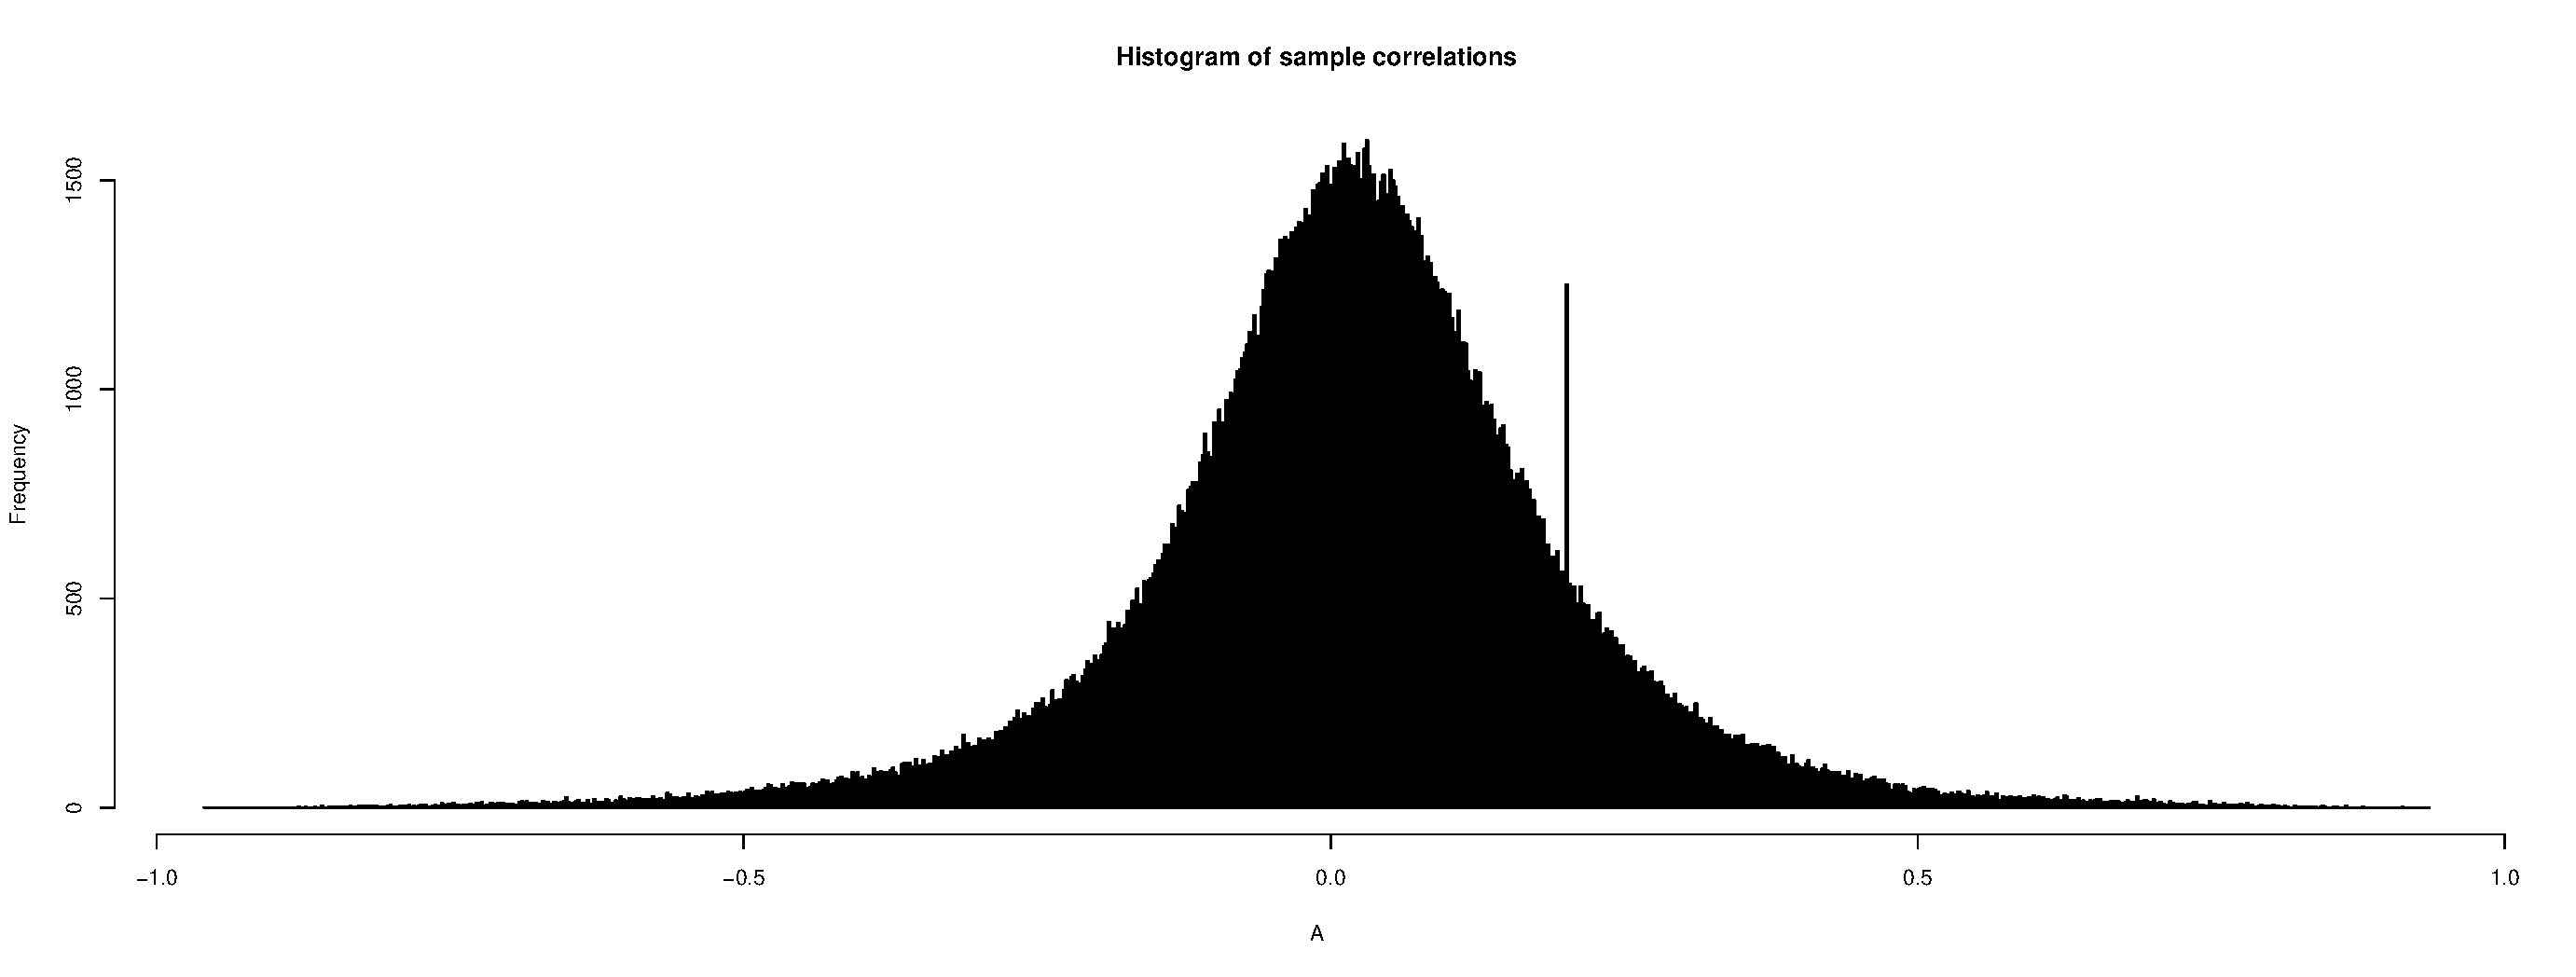
\includegraphics[width = 1\textwidth]{corr_hist}\\
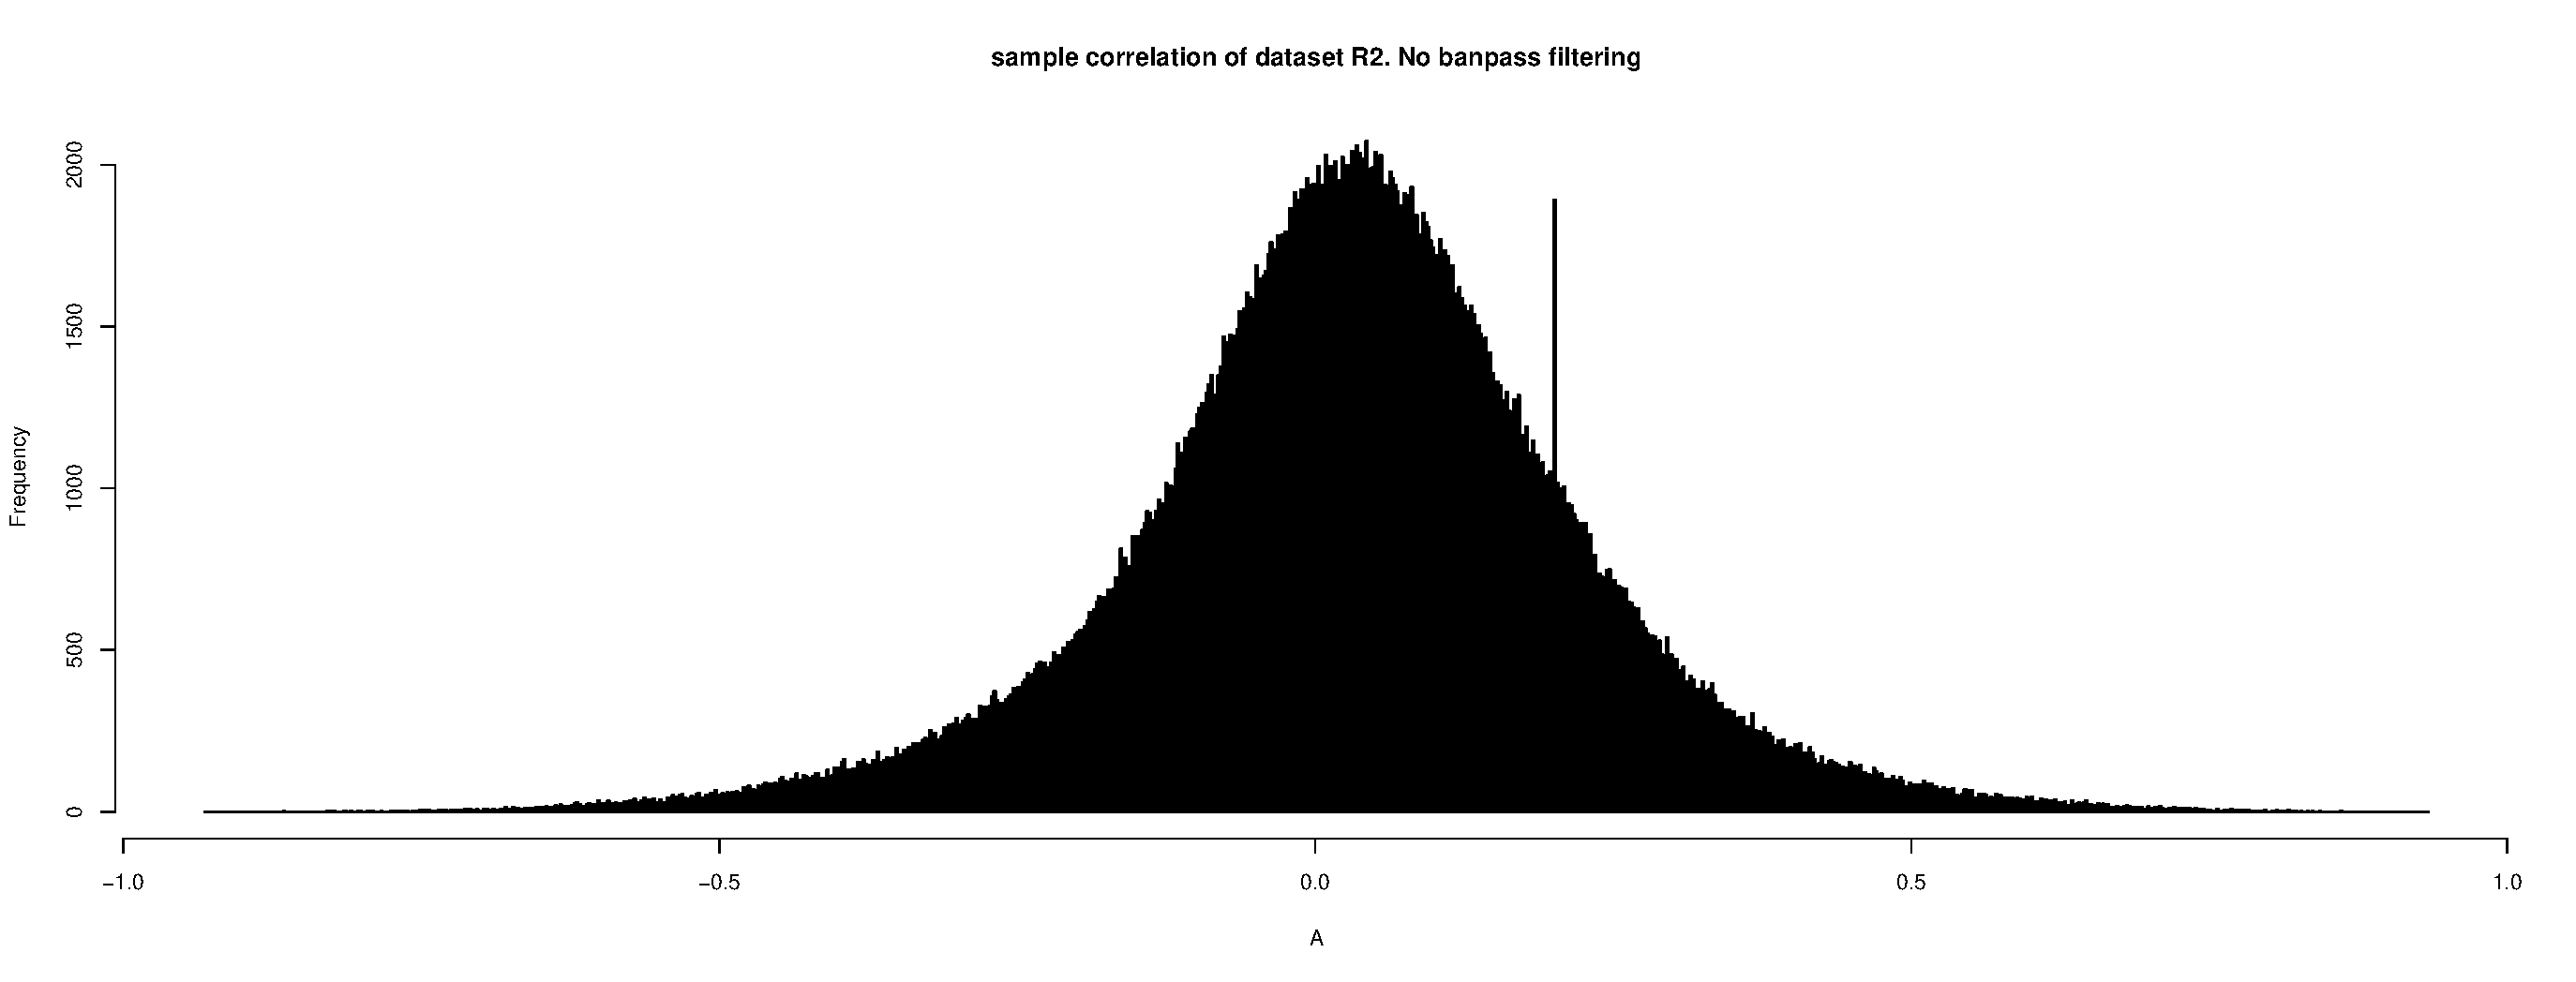
\includegraphics[width = 1\textwidth]{figures2/corr_hist_nofilter_R2}
\caption{histogram of sample correlation of fMRI dataset R1 and R2. top is R1. Bottom is R2.  It is unimodal, with mean slightly away from zero. The sharp bump around 0.2 is the connection of a voxel with itself, and I set it manually to 0.2, a empirical value that falls into the mixture model.}
\label{fig101}
\end{figure}

\textbf{connectivity map with different seed voxels: } See figure \ref{fig102}.
\begin{figure}[htb]
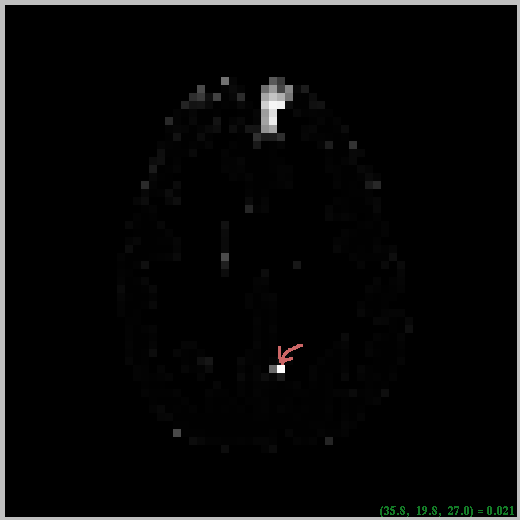
\includegraphics[width = 0.3\textwidth]{probe1}
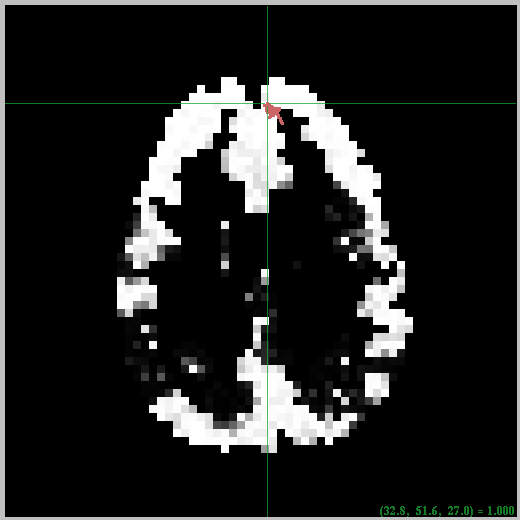
\includegraphics[width = 0.3\textwidth]{probe2}
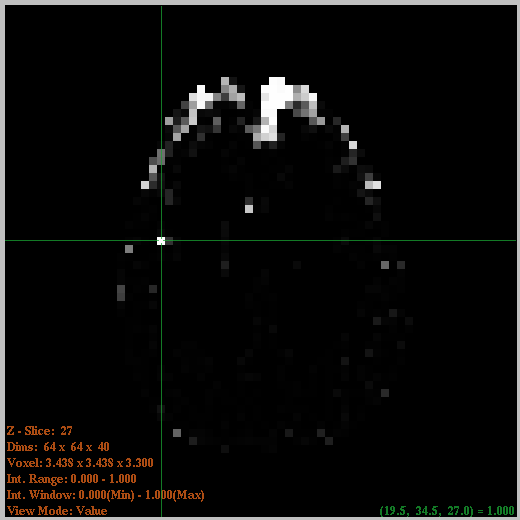
\includegraphics[width = 0.3\textwidth]{probe3}
\caption{connectivity map with different seed voxels.}
\label{fig102}
\end{figure}

\textbf{bandpass filtering: } our data set TR = 2s. In 'functional connectivity premier', the cutoff frequency $f_H = 0.08 Hz$, $f_L = 0.009 Hz$.  for low pass filtering, $0.08 Hz \rightarrow 12.5s \approx 6 TR$. For hight pass filtering, $0.009Hz \rightarrow 111s \approx 55 TR$.

\textbf{estimation of parameters $\mu$ and $\sigma$: } See log files. 

\textbf{Histogram of sample correlation after bandpass filtering: } See figure \ref{fig103}. There are more positive correlatd and negative correlated connectivity than before filtering. To see if this change of histogram is caused by high pass filtering, or low pass filtering. I need to filter time series by either of them and see the results. A simple test found even only with low pass filter, the histogram of filtered data is much like bandpass filtered data. That mean removing high frequency component of time series siginficantly changed the histogram of correlation.

\textbf{Time and frequency domain response before and after bandpass filtering: } See figure \ref{fig104}.

\textbf{corrlation map before and after bandpass filtering; } See figure \ref{fig105}.


\begin{figure}[htb]
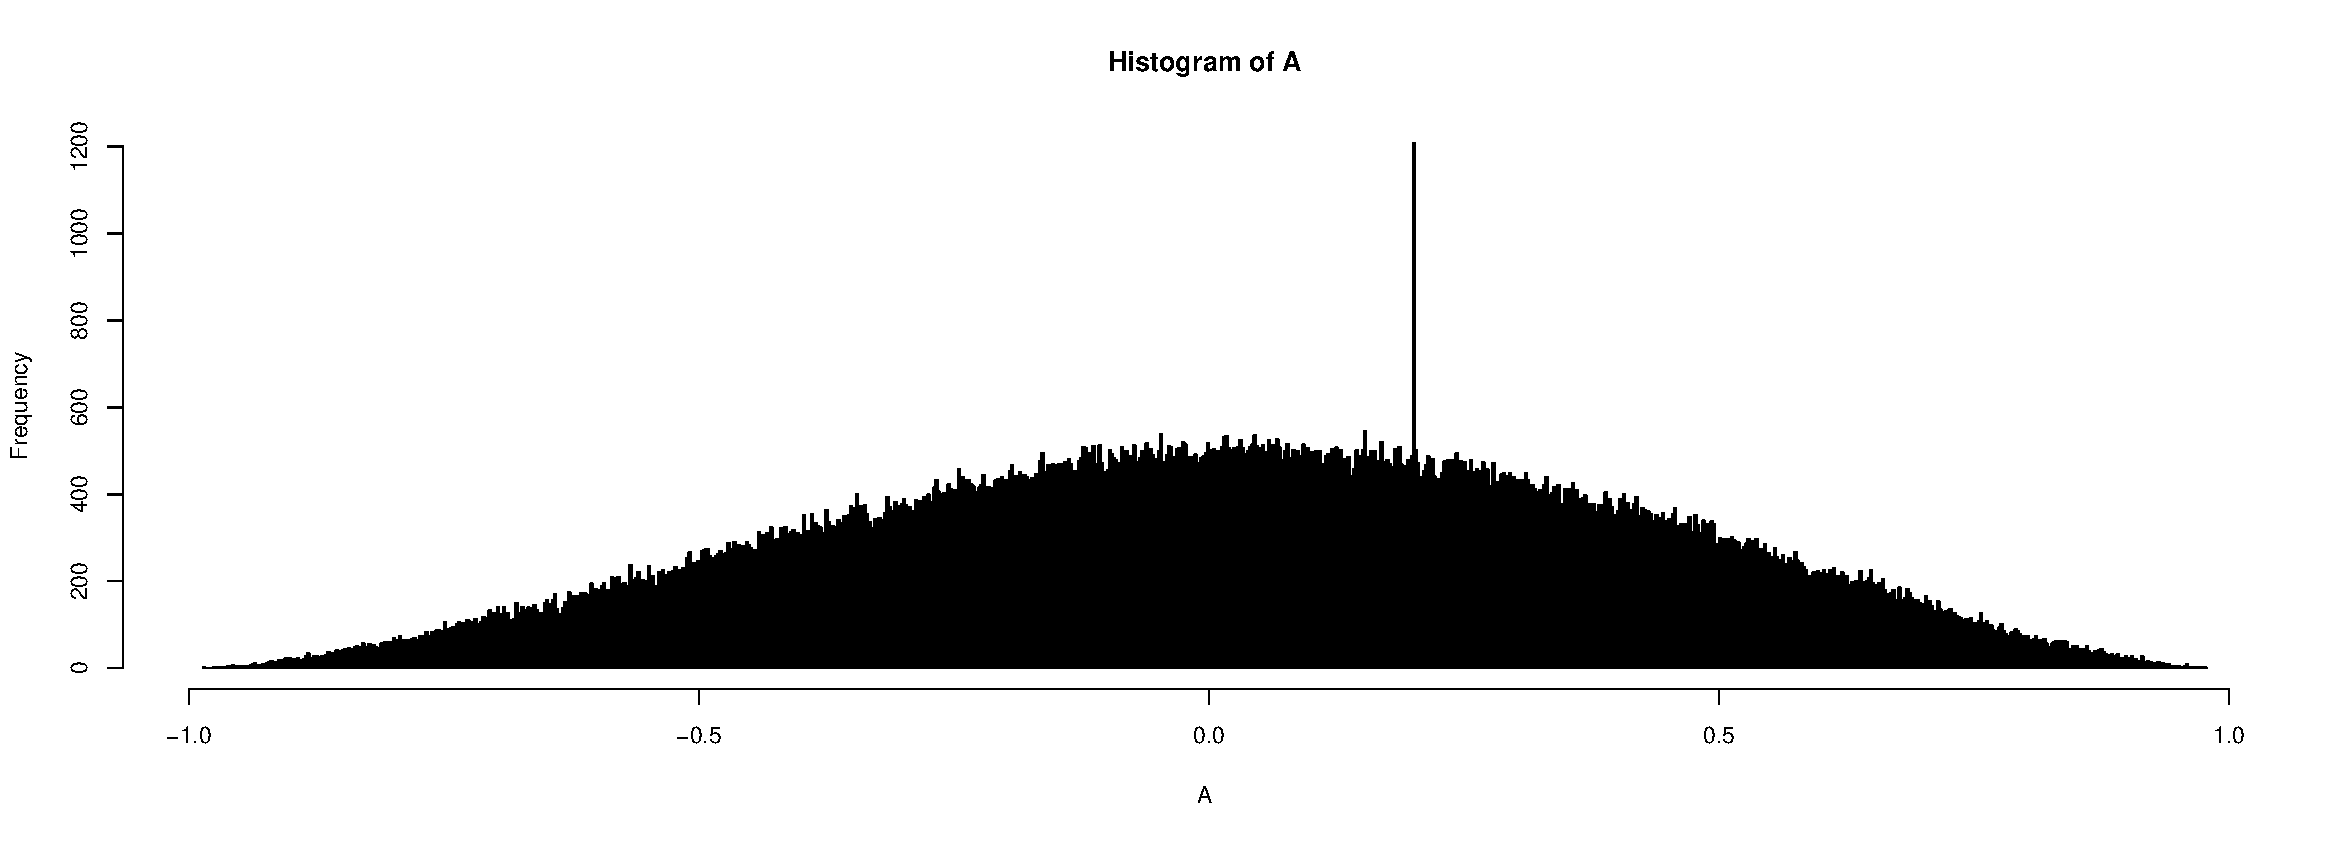
\includegraphics[width = 1\textwidth]{corr_hist_filtered}\\
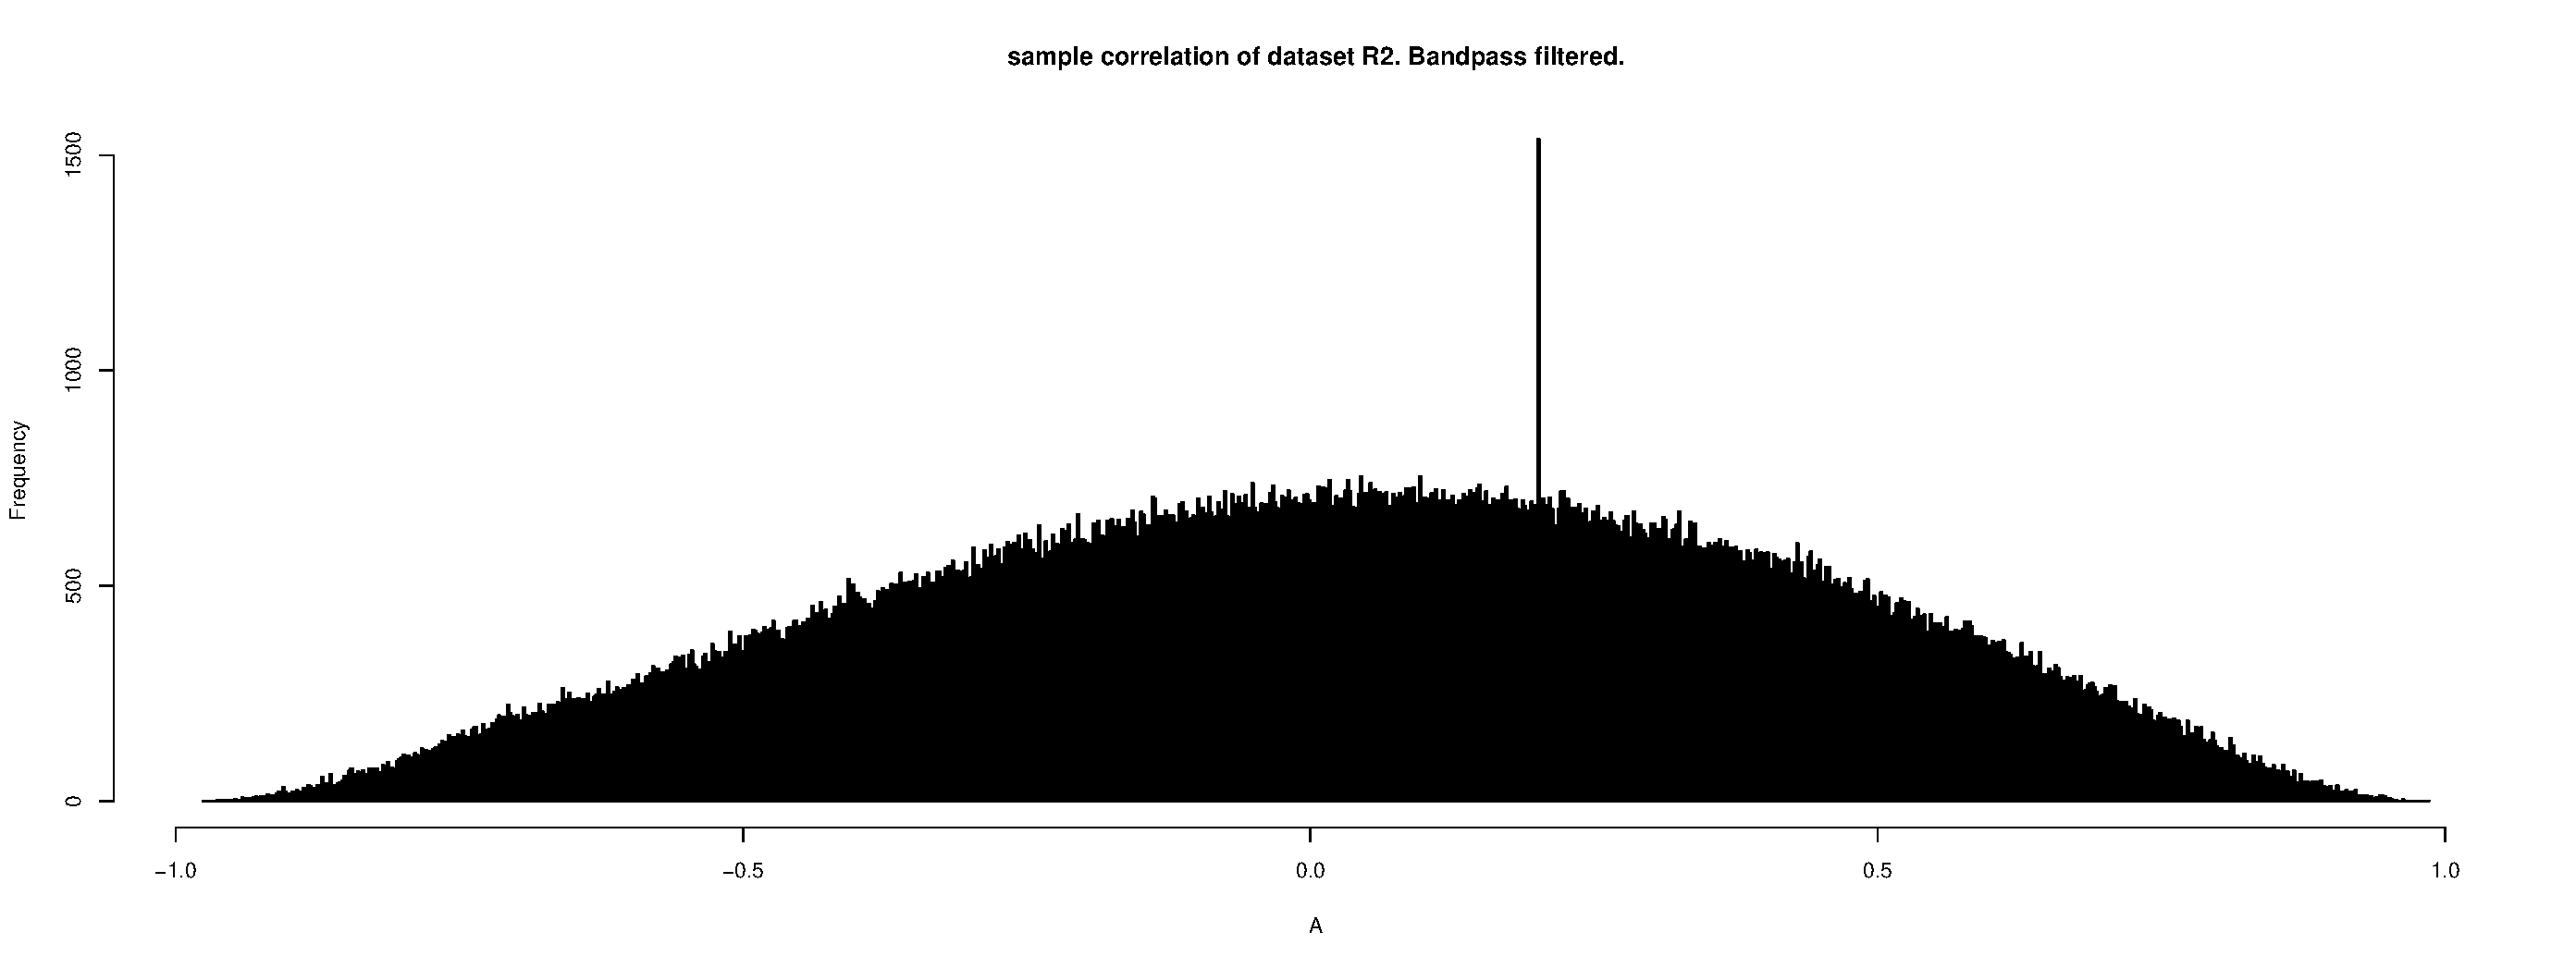
\includegraphics[width = 1\textwidth]{figures2/corr_hist_filtered_R2}
\caption{Histogram of sample correlation after bandpass filtering. Top is dataset R1, bottom is dataset R2.}
\label{fig103}
\end{figure}

\begin{figure}[htb]
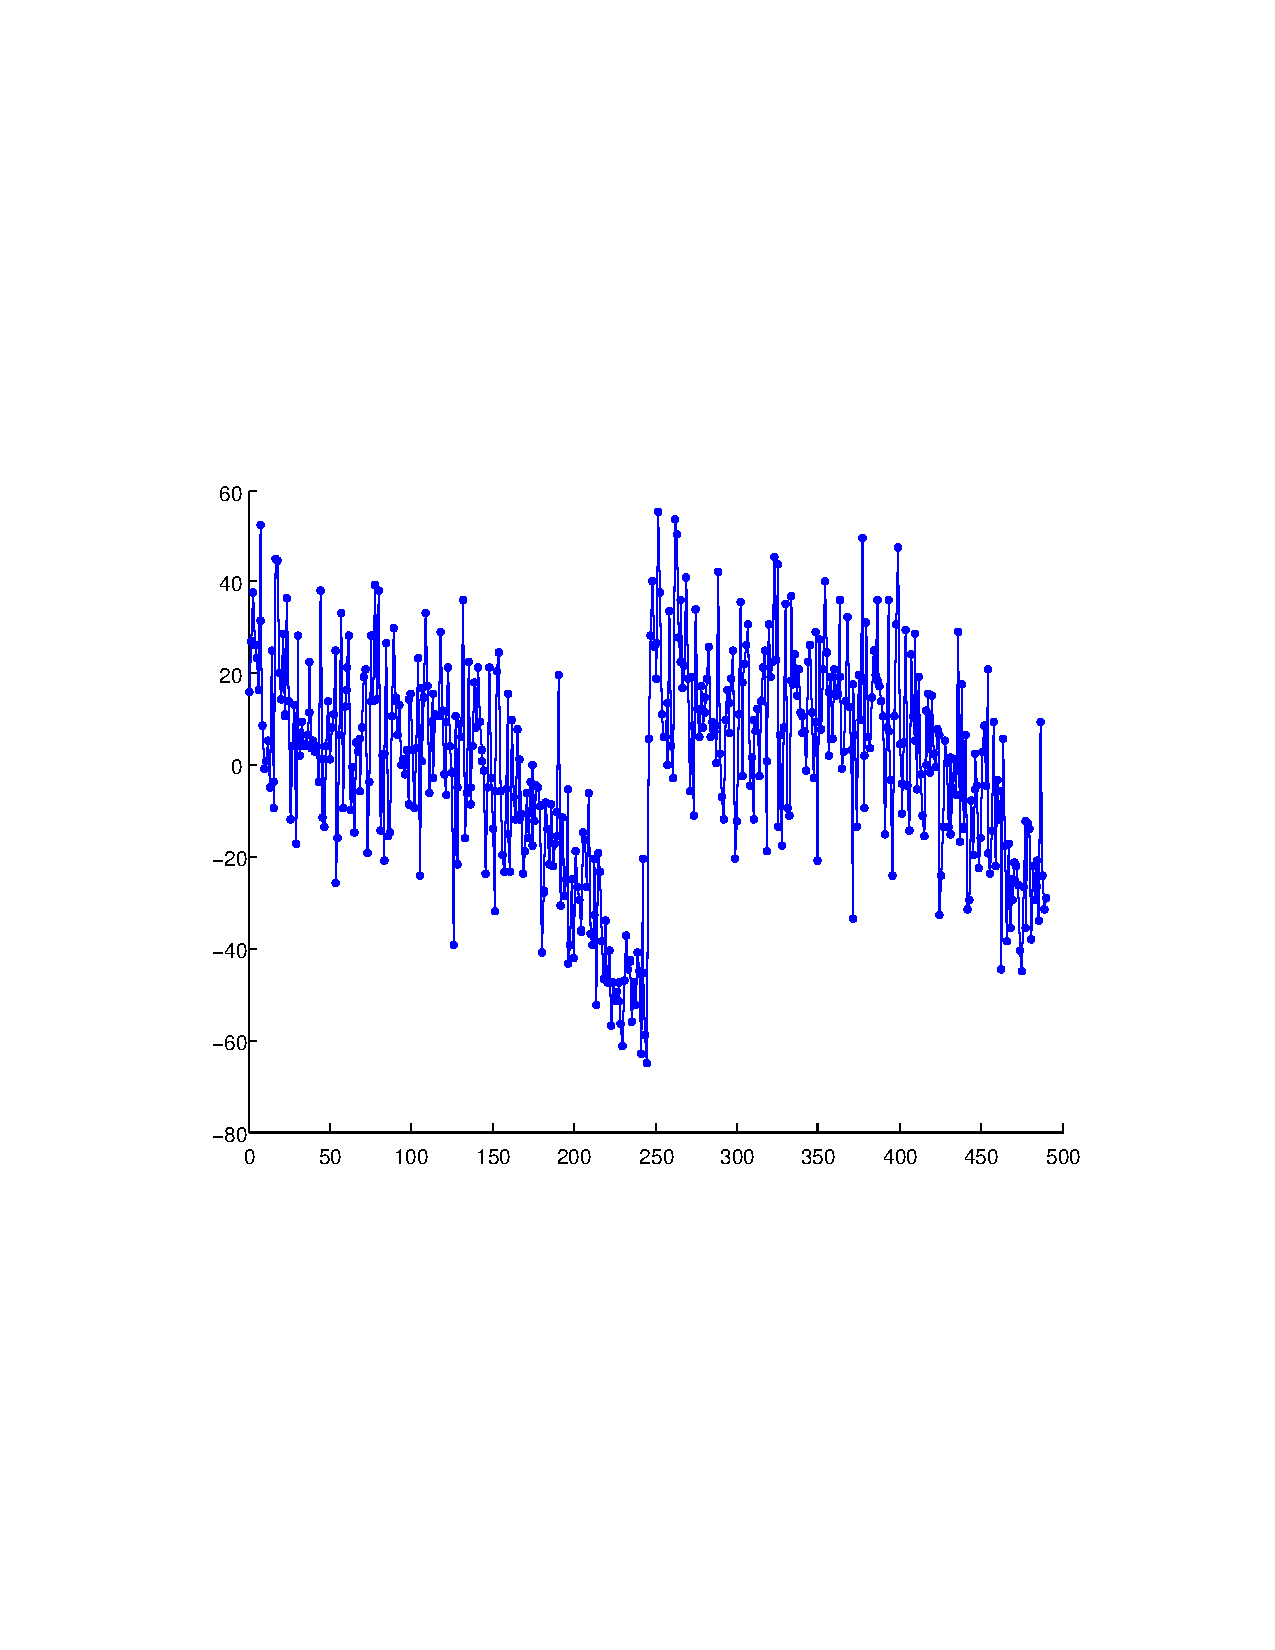
\includegraphics[width = 0.24\textwidth]{figures2/ts_before_1}
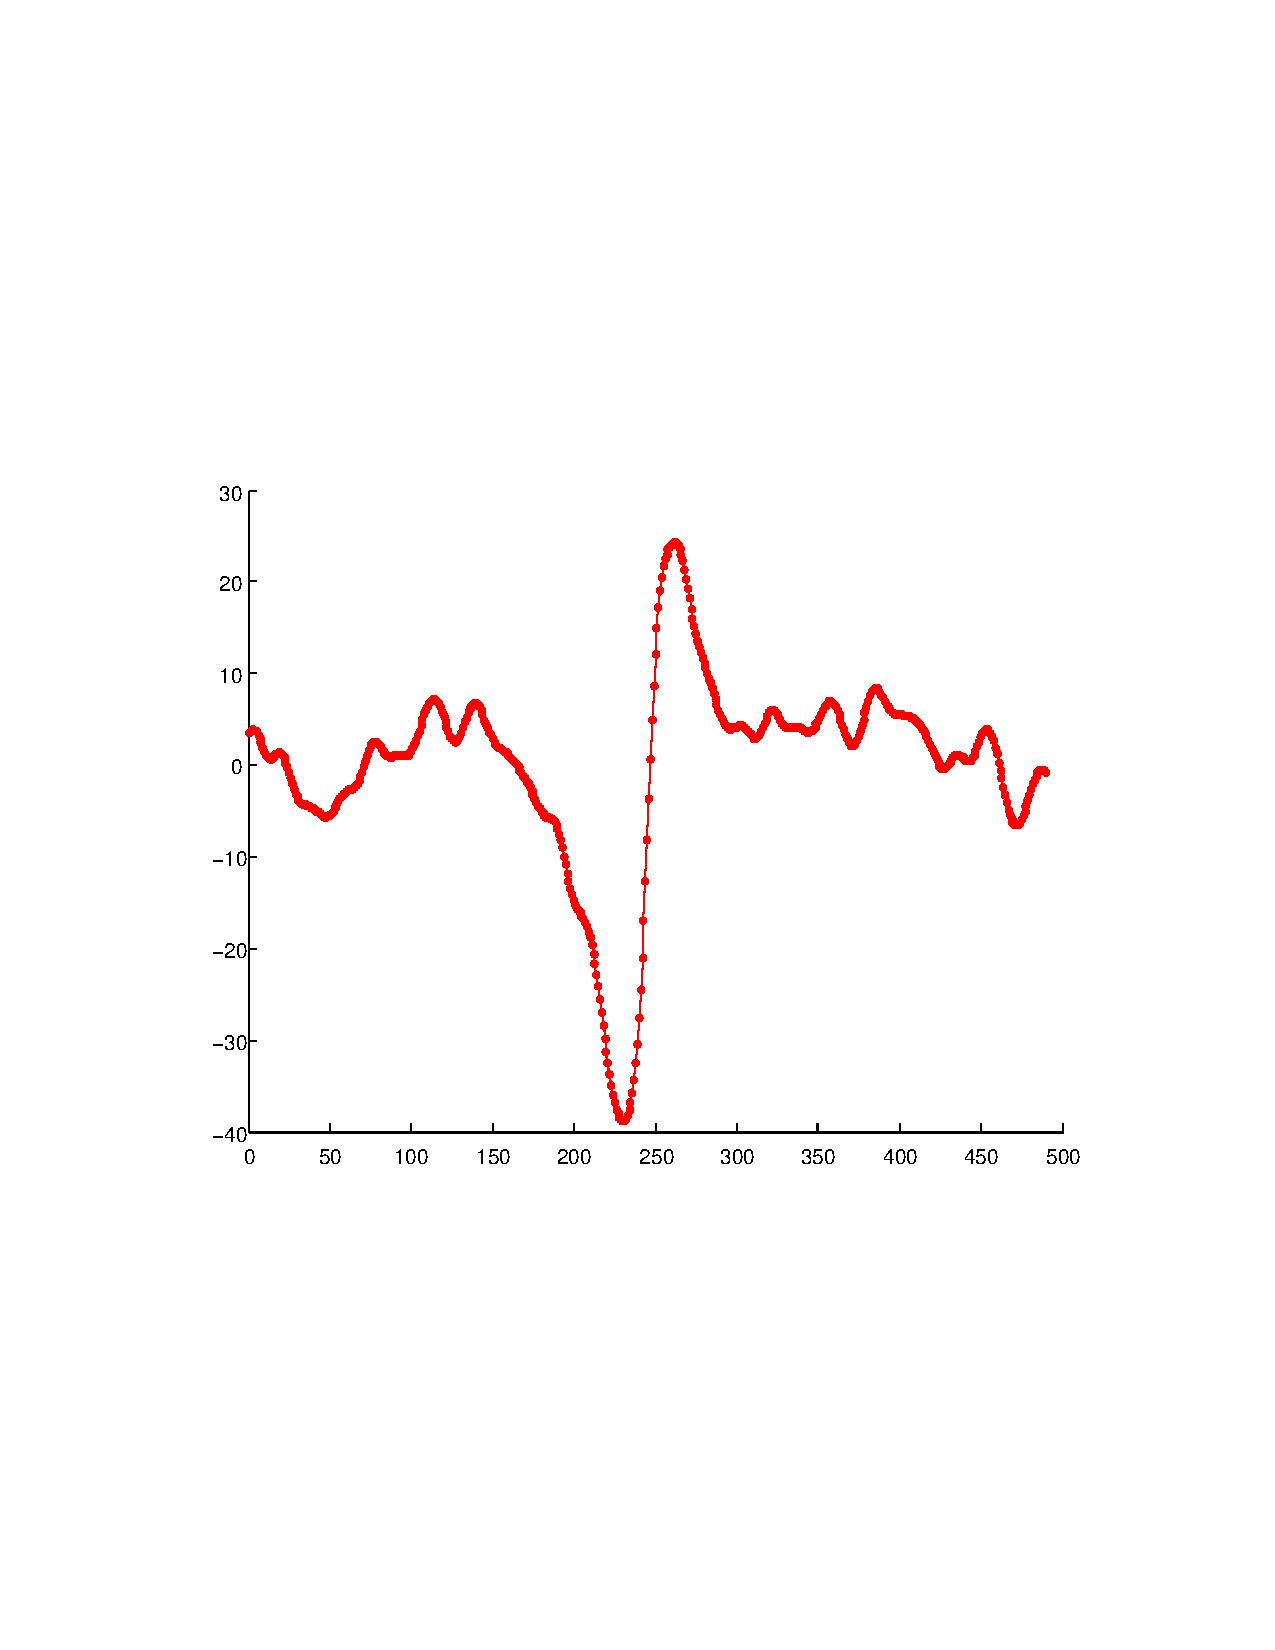
\includegraphics[width = 0.24\textwidth]{figures2/ts_after_1}
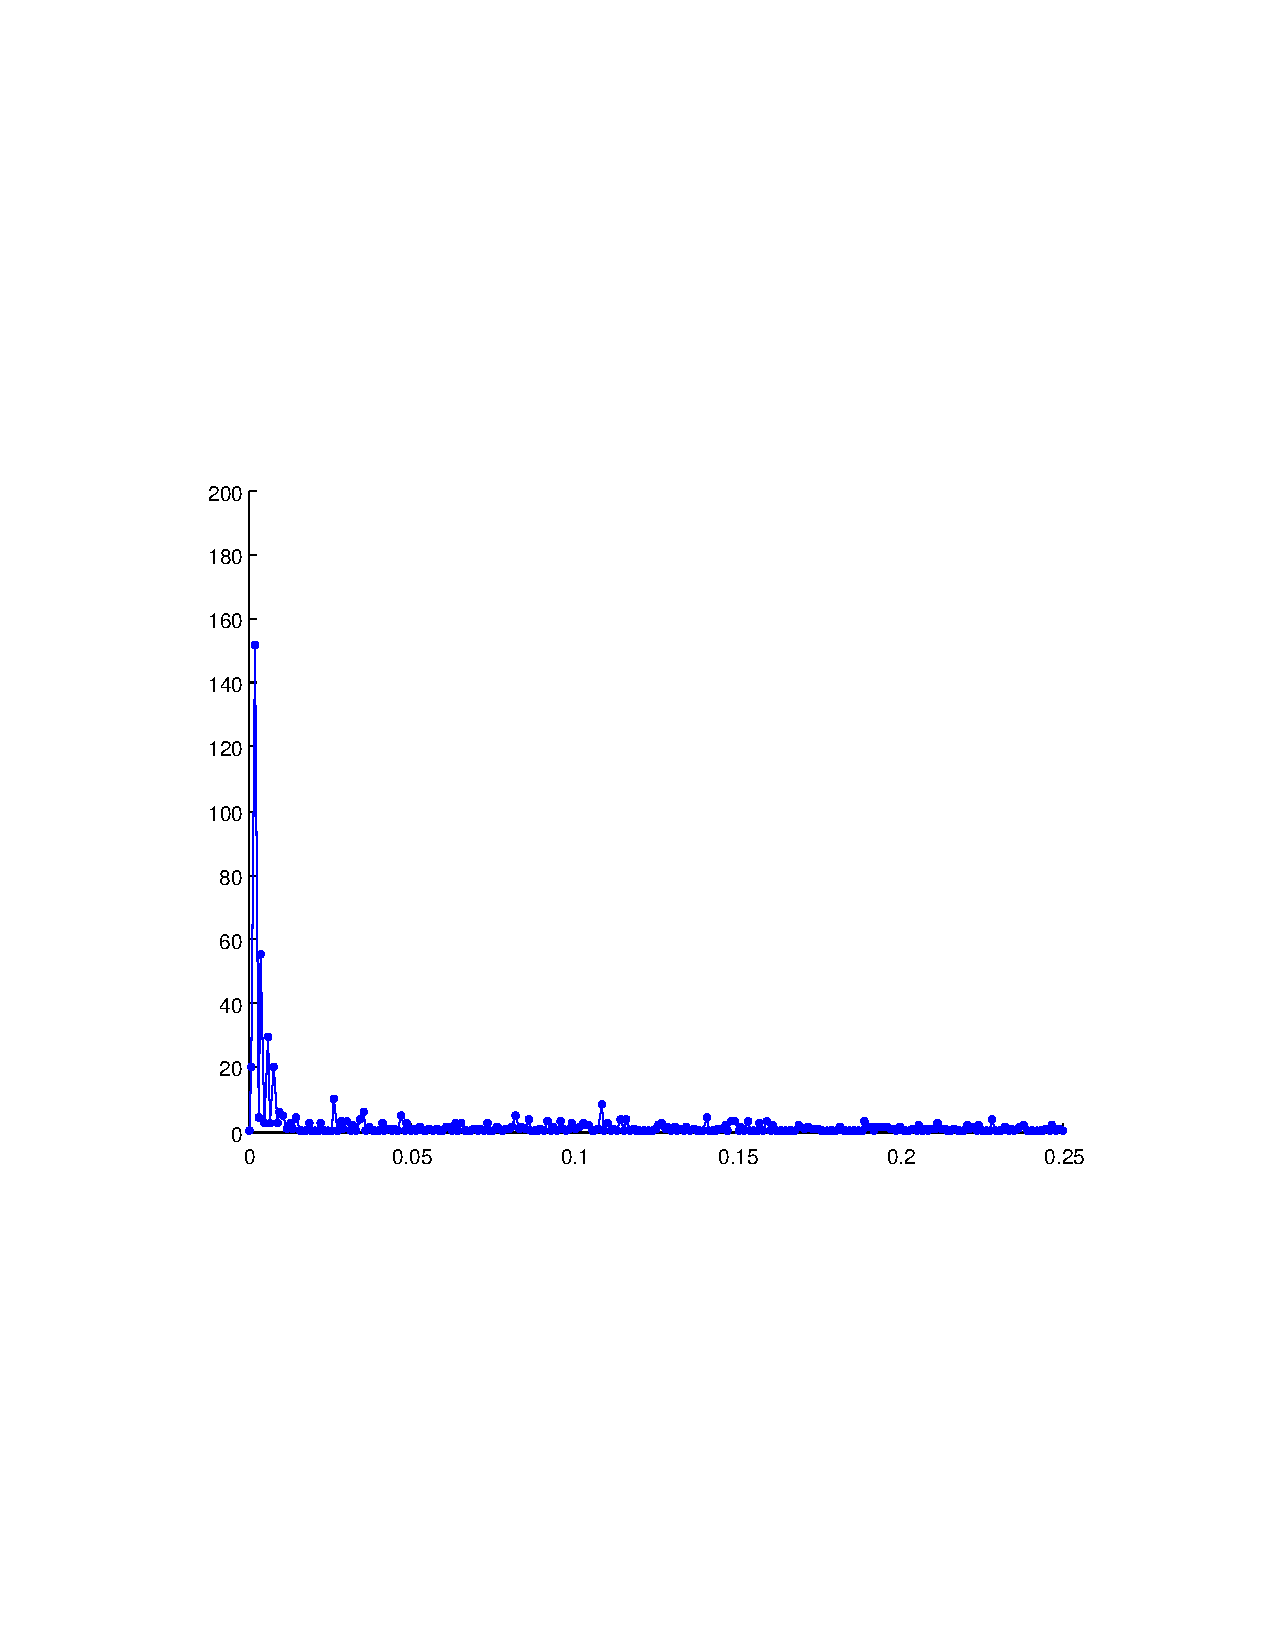
\includegraphics[width = 0.24\textwidth]{figures2/freq_before_1}
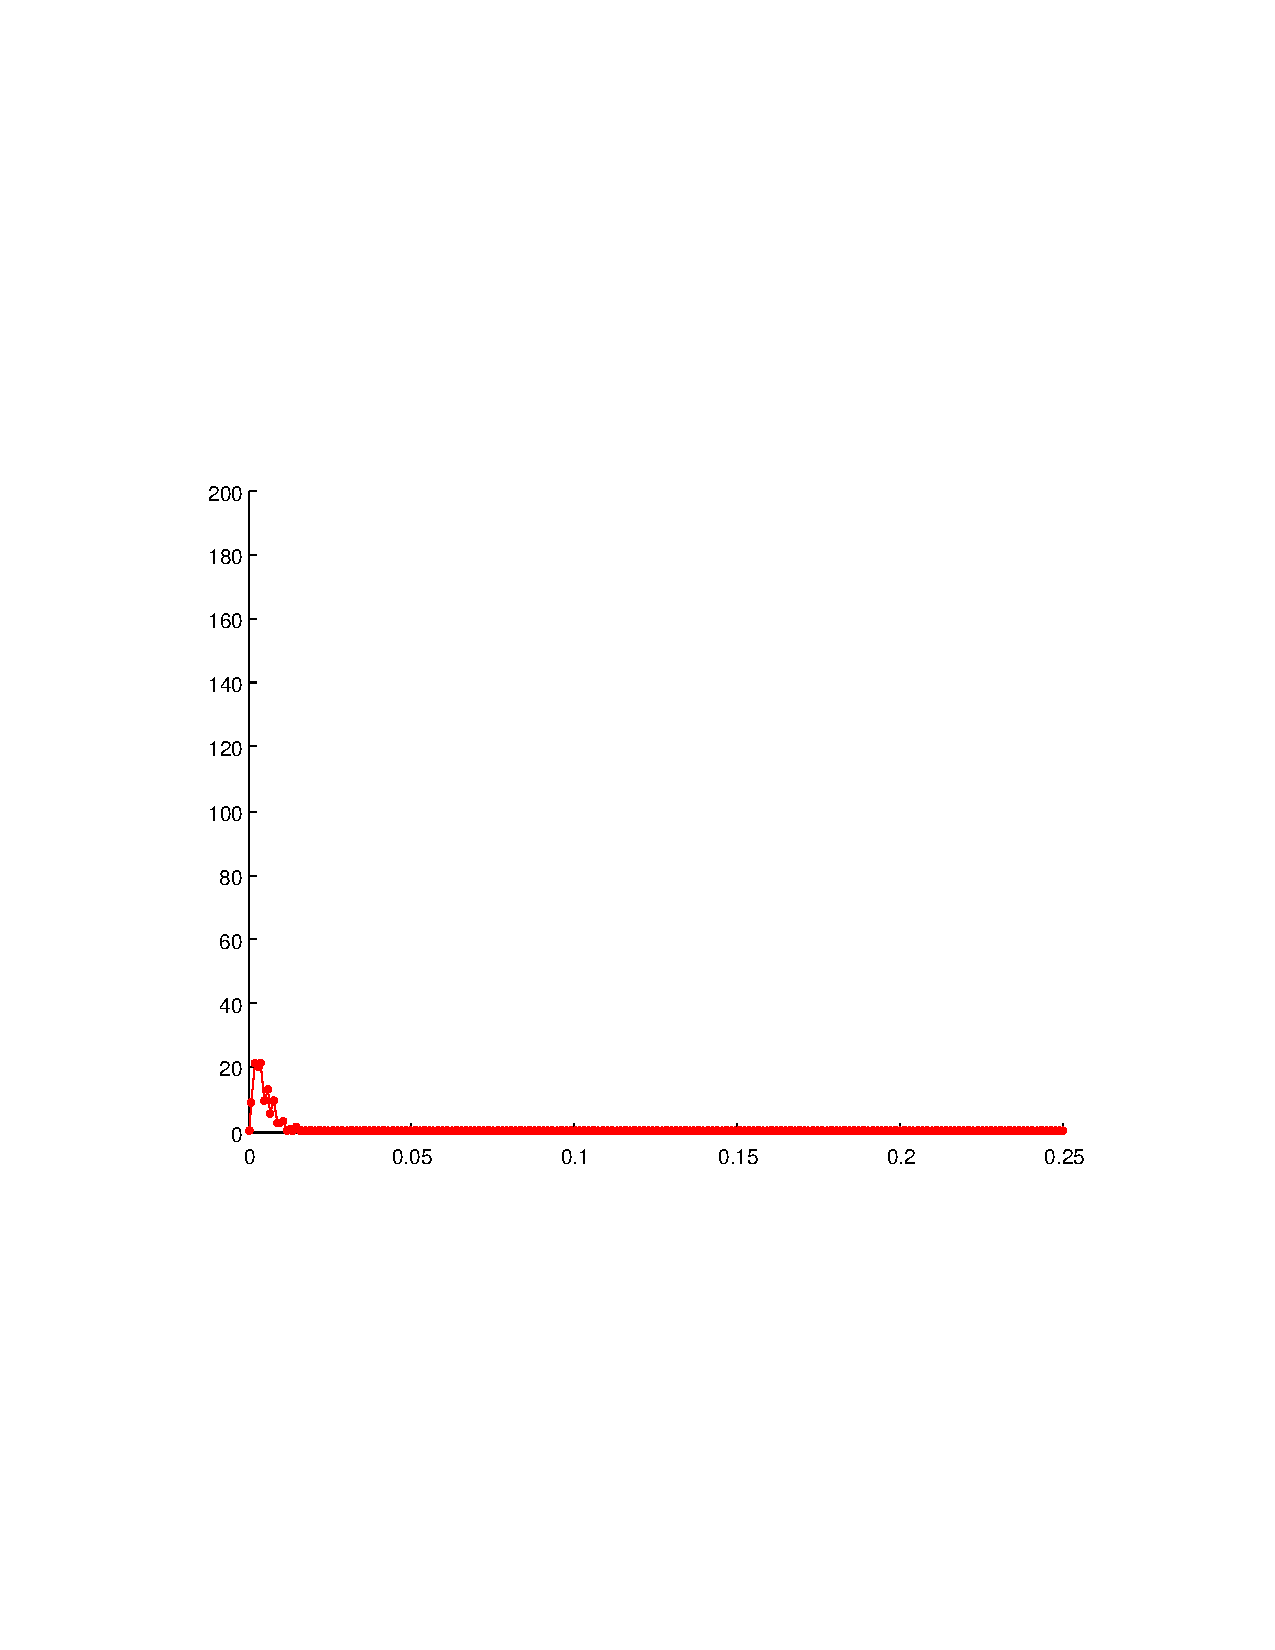
\includegraphics[width = 0.24\textwidth]{figures2/freq_after_1}\\
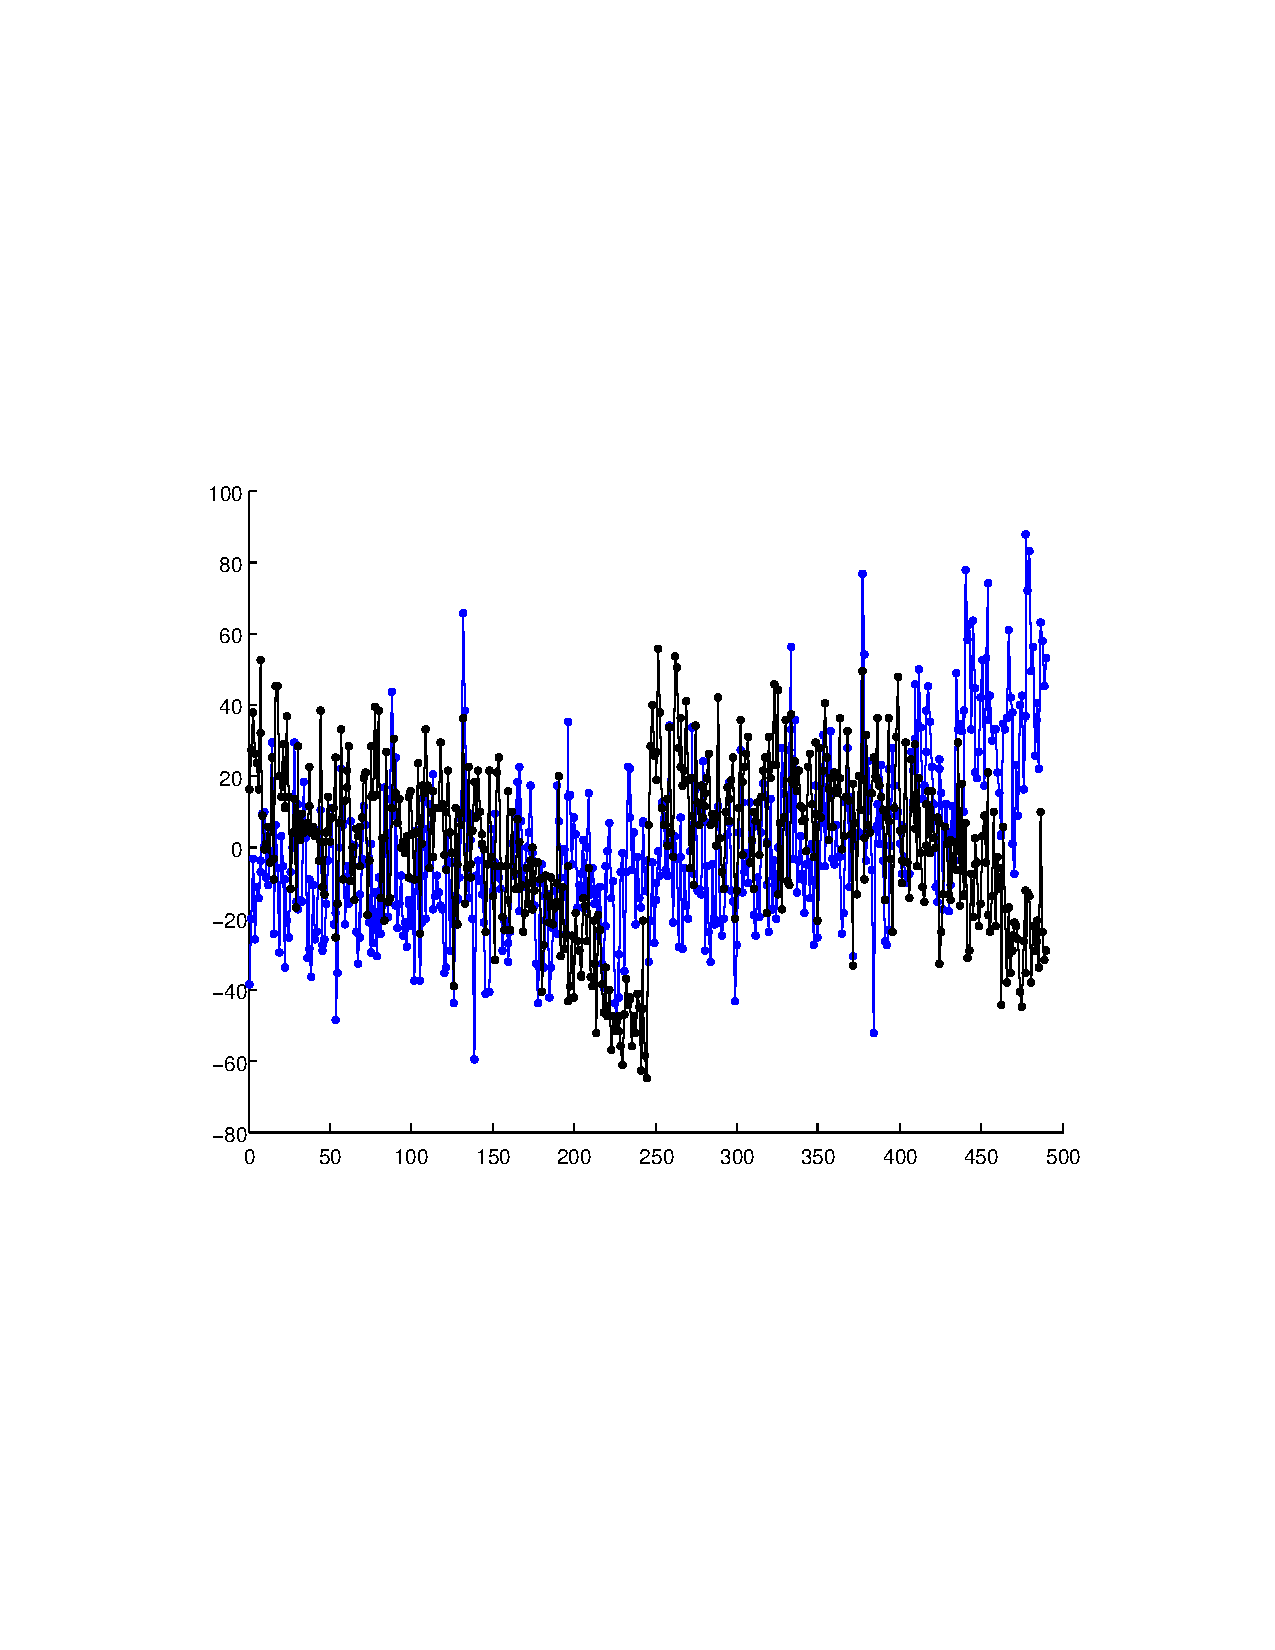
\includegraphics[width = 0.24\textwidth]{figures2/ts_before_2}
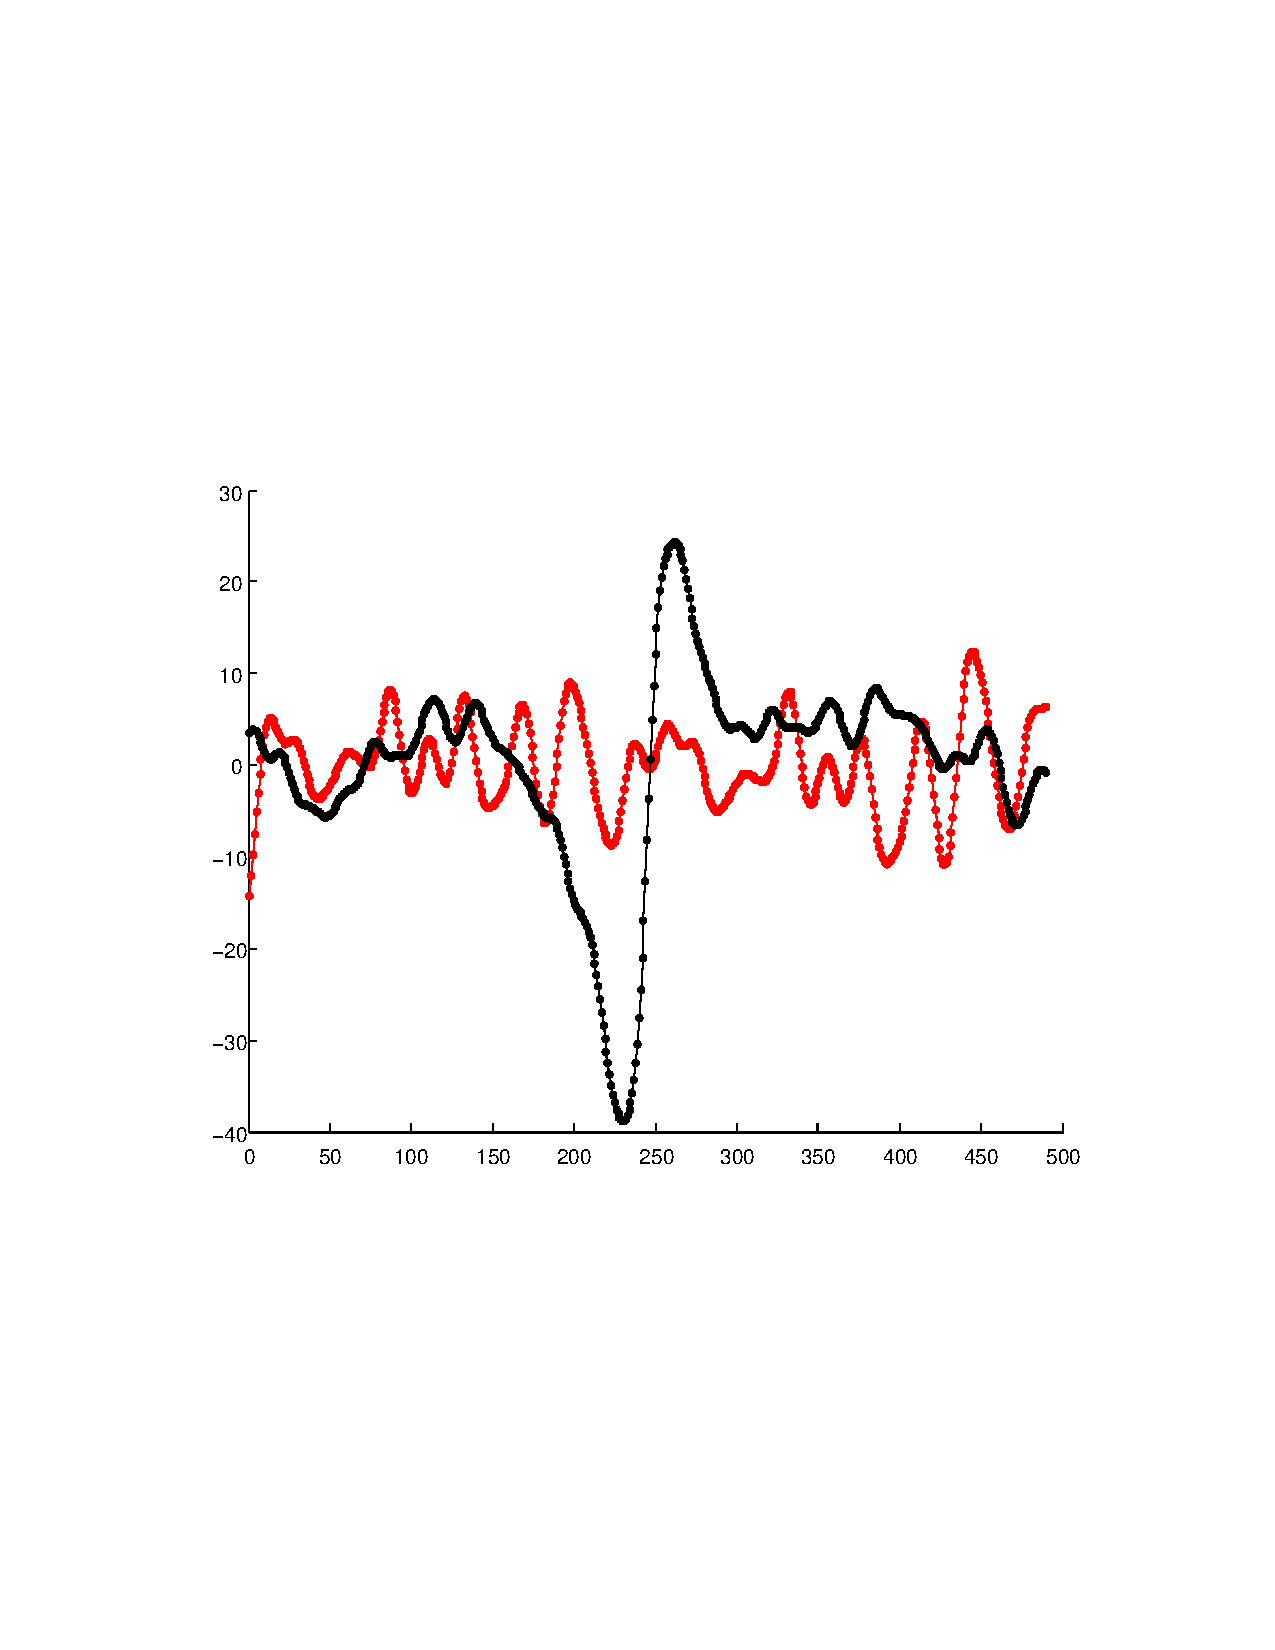
\includegraphics[width = 0.24\textwidth]{figures2/ts_after_2}
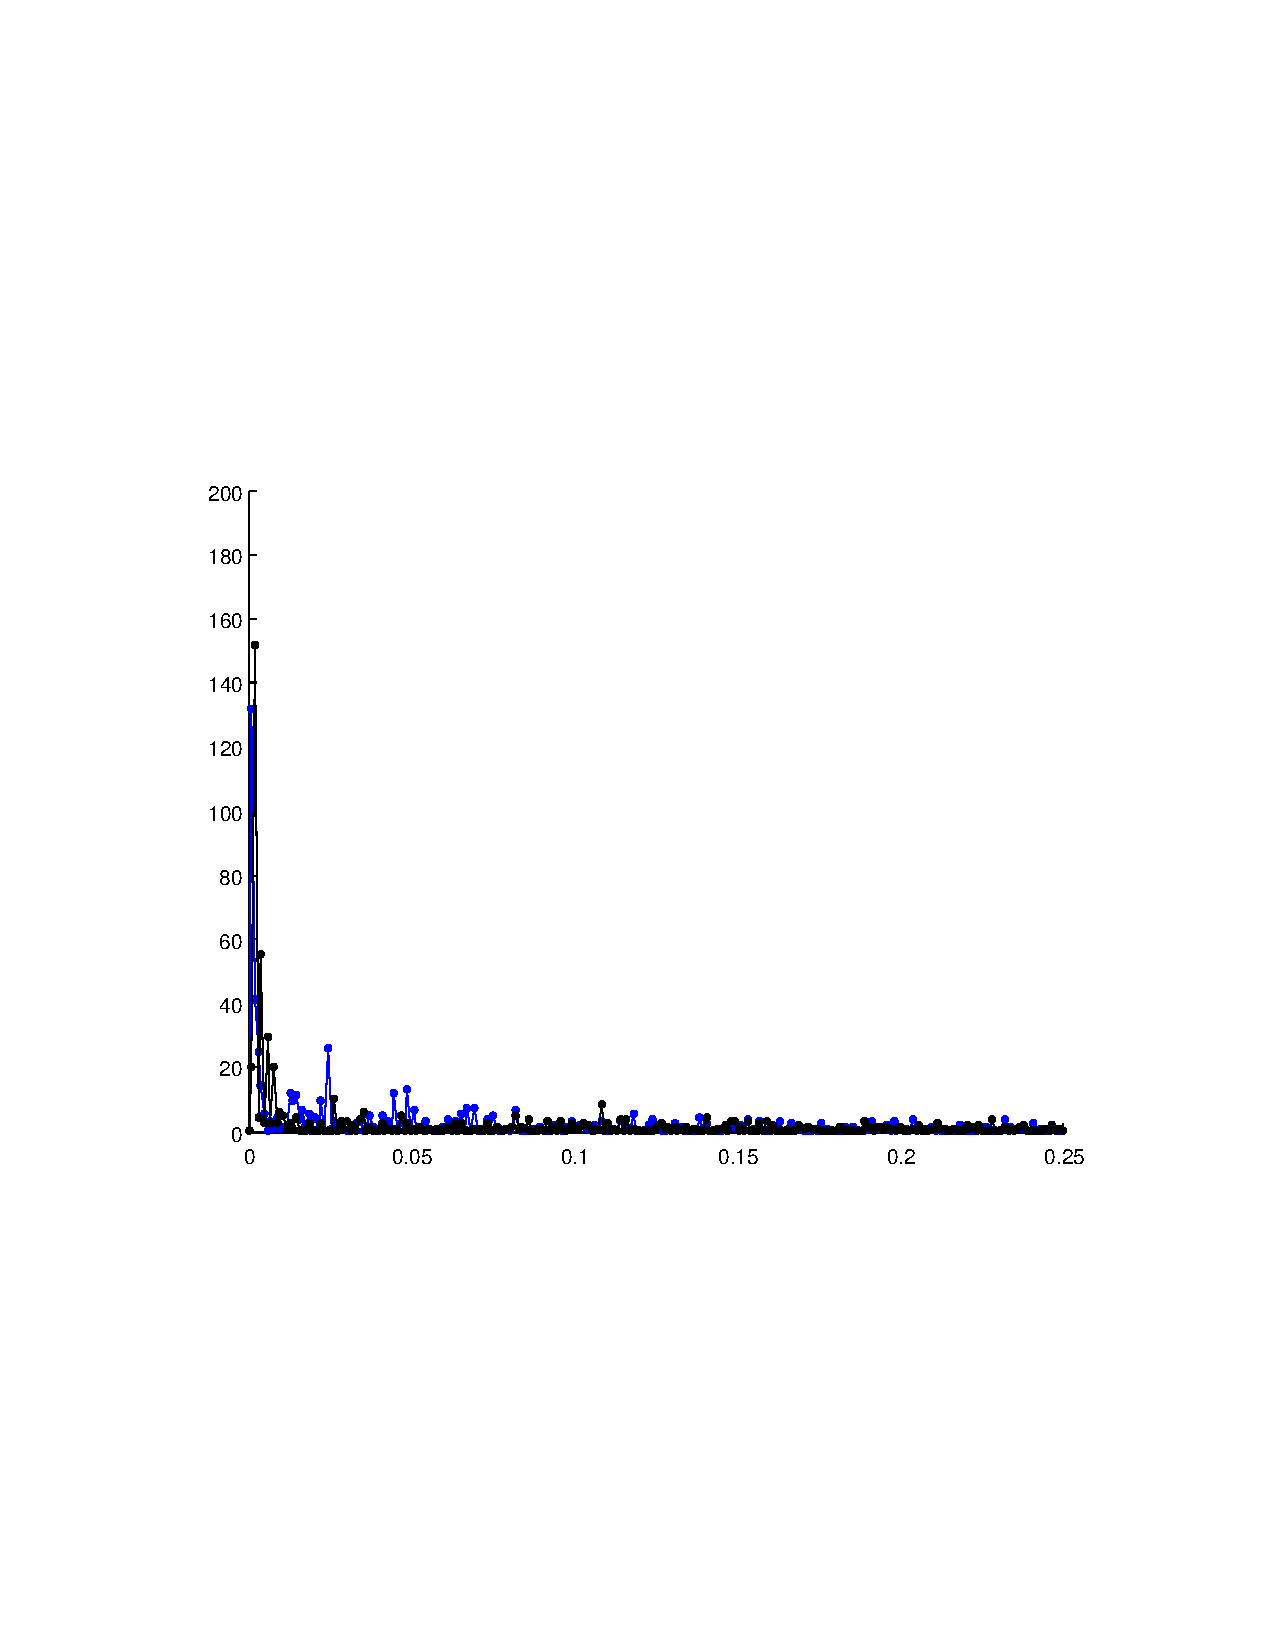
\includegraphics[width = 0.24\textwidth]{figures2/freq_before_2}
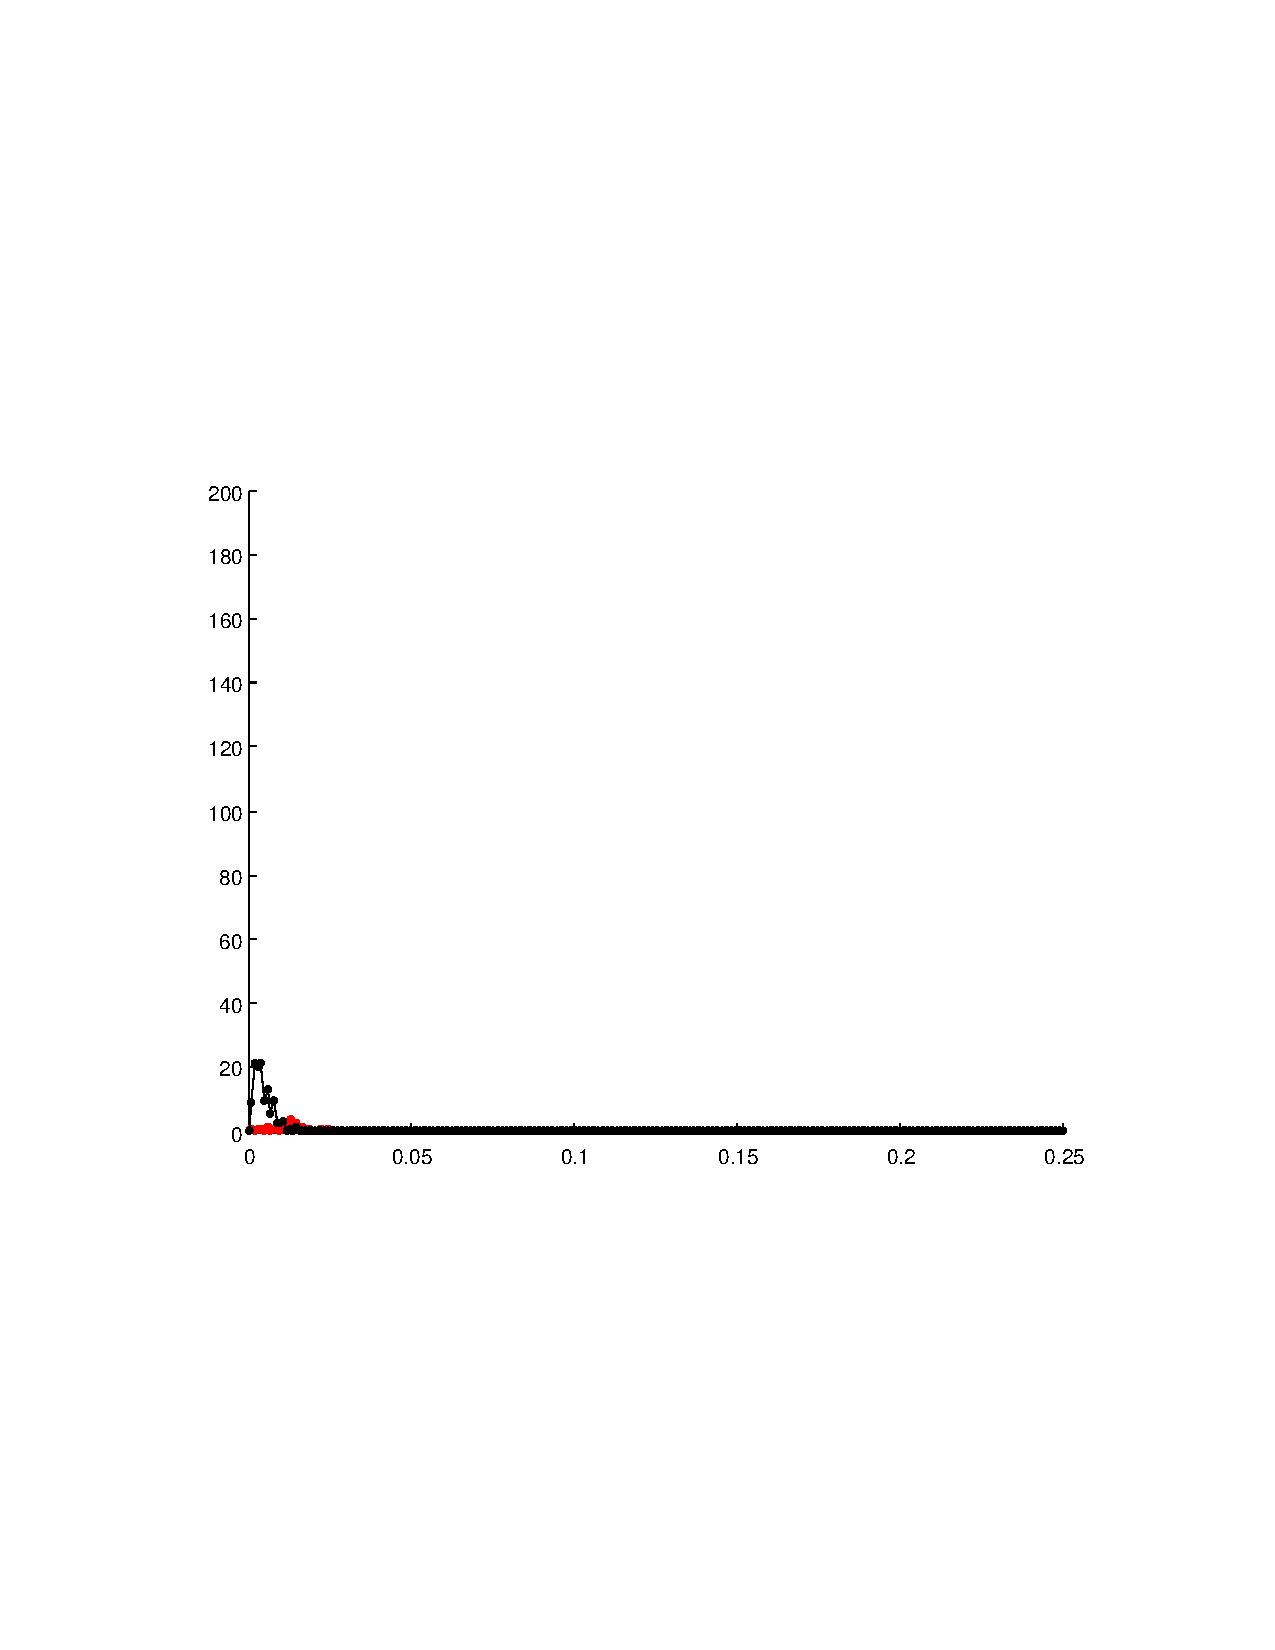
\includegraphics[width = 0.24\textwidth]{figures2/freq_after_2} \\
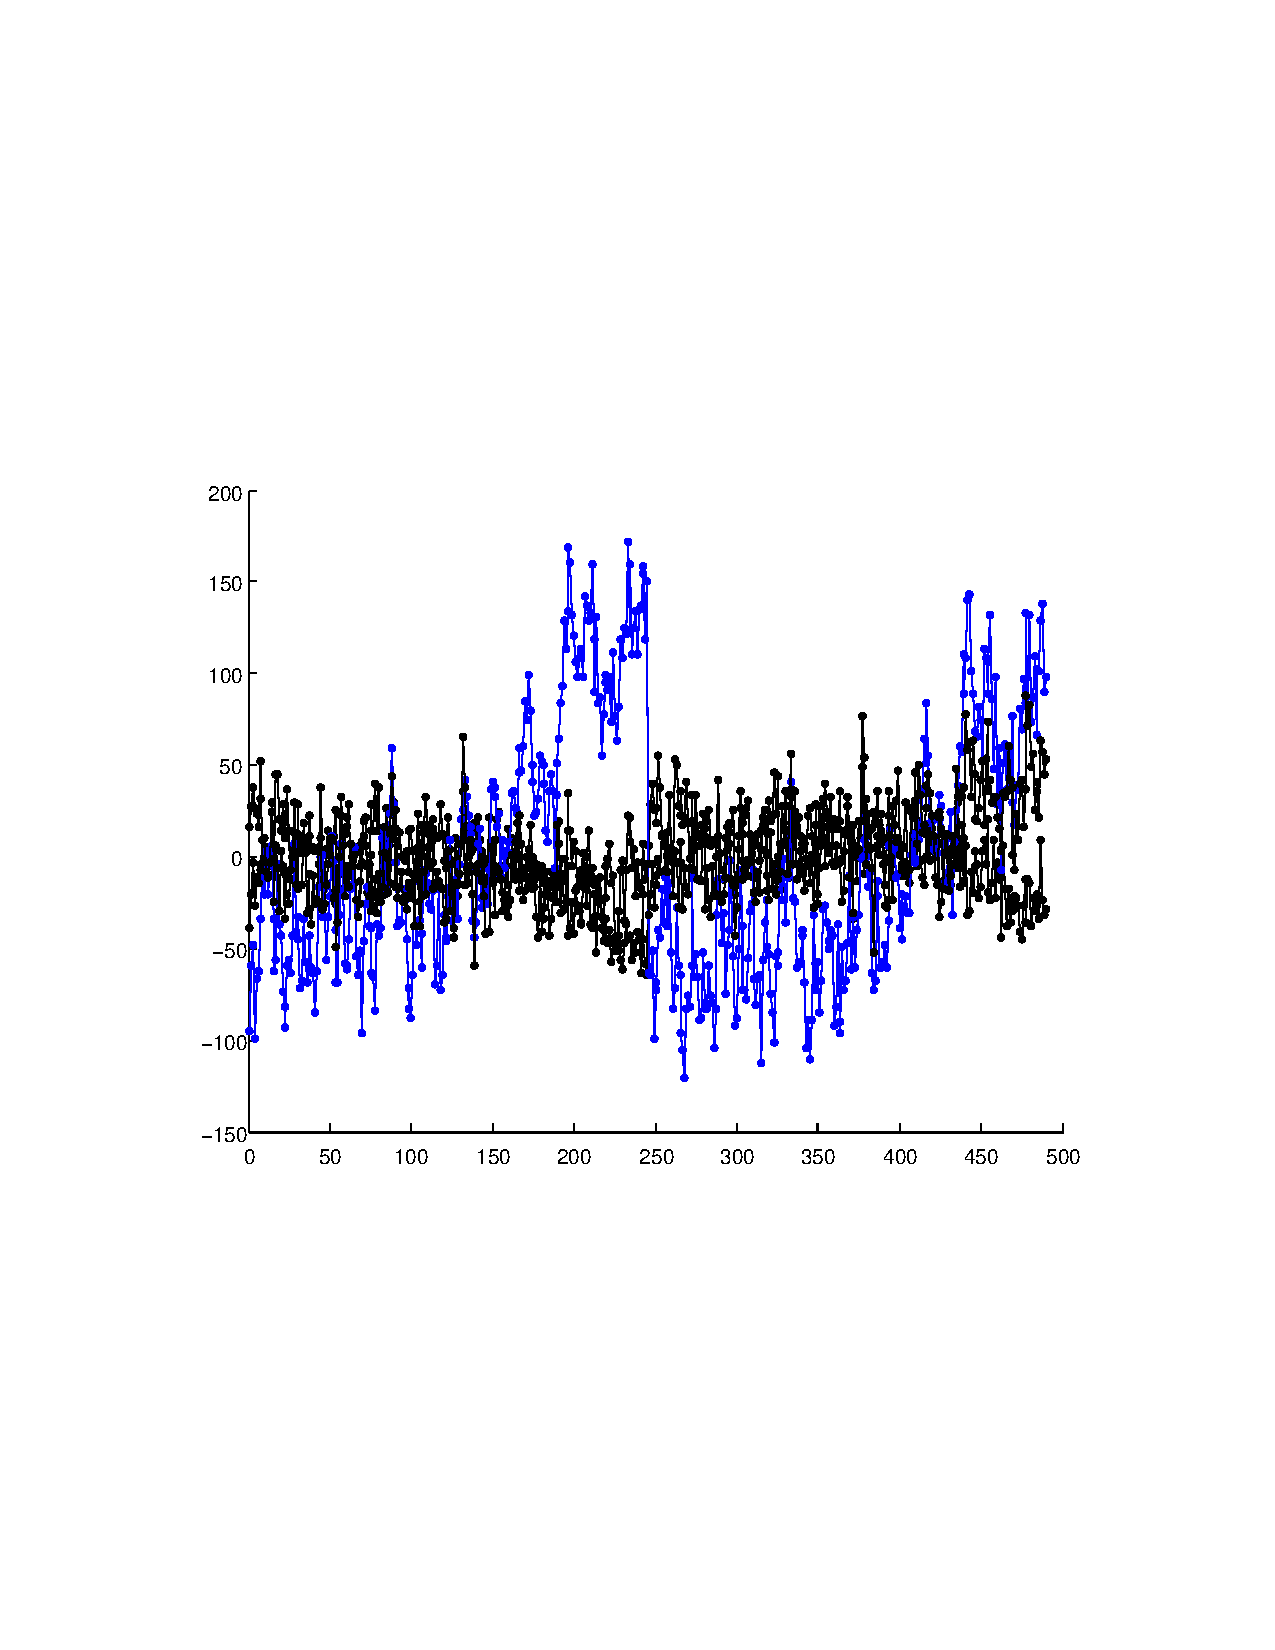
\includegraphics[width = 0.24\textwidth]{figures2/ts_before_3}
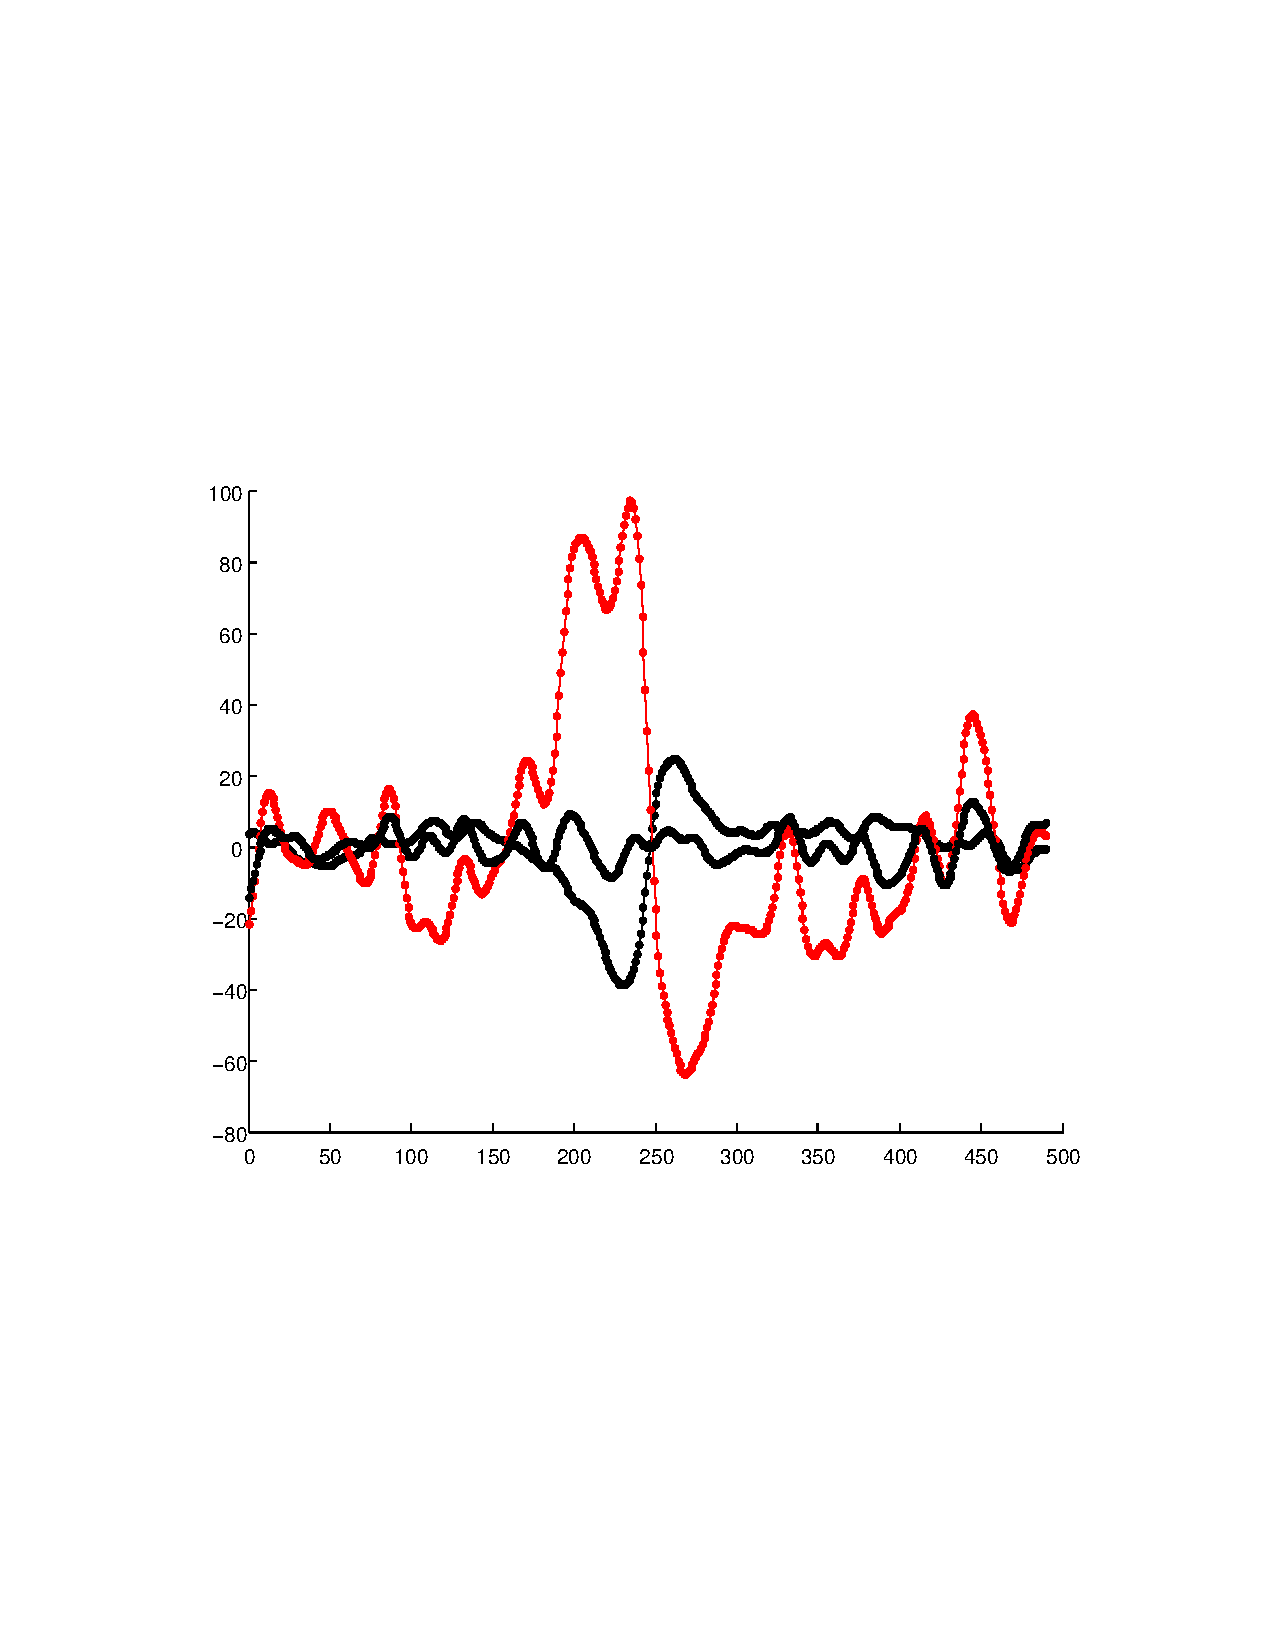
\includegraphics[width = 0.24\textwidth]{figures2/ts_after_3}
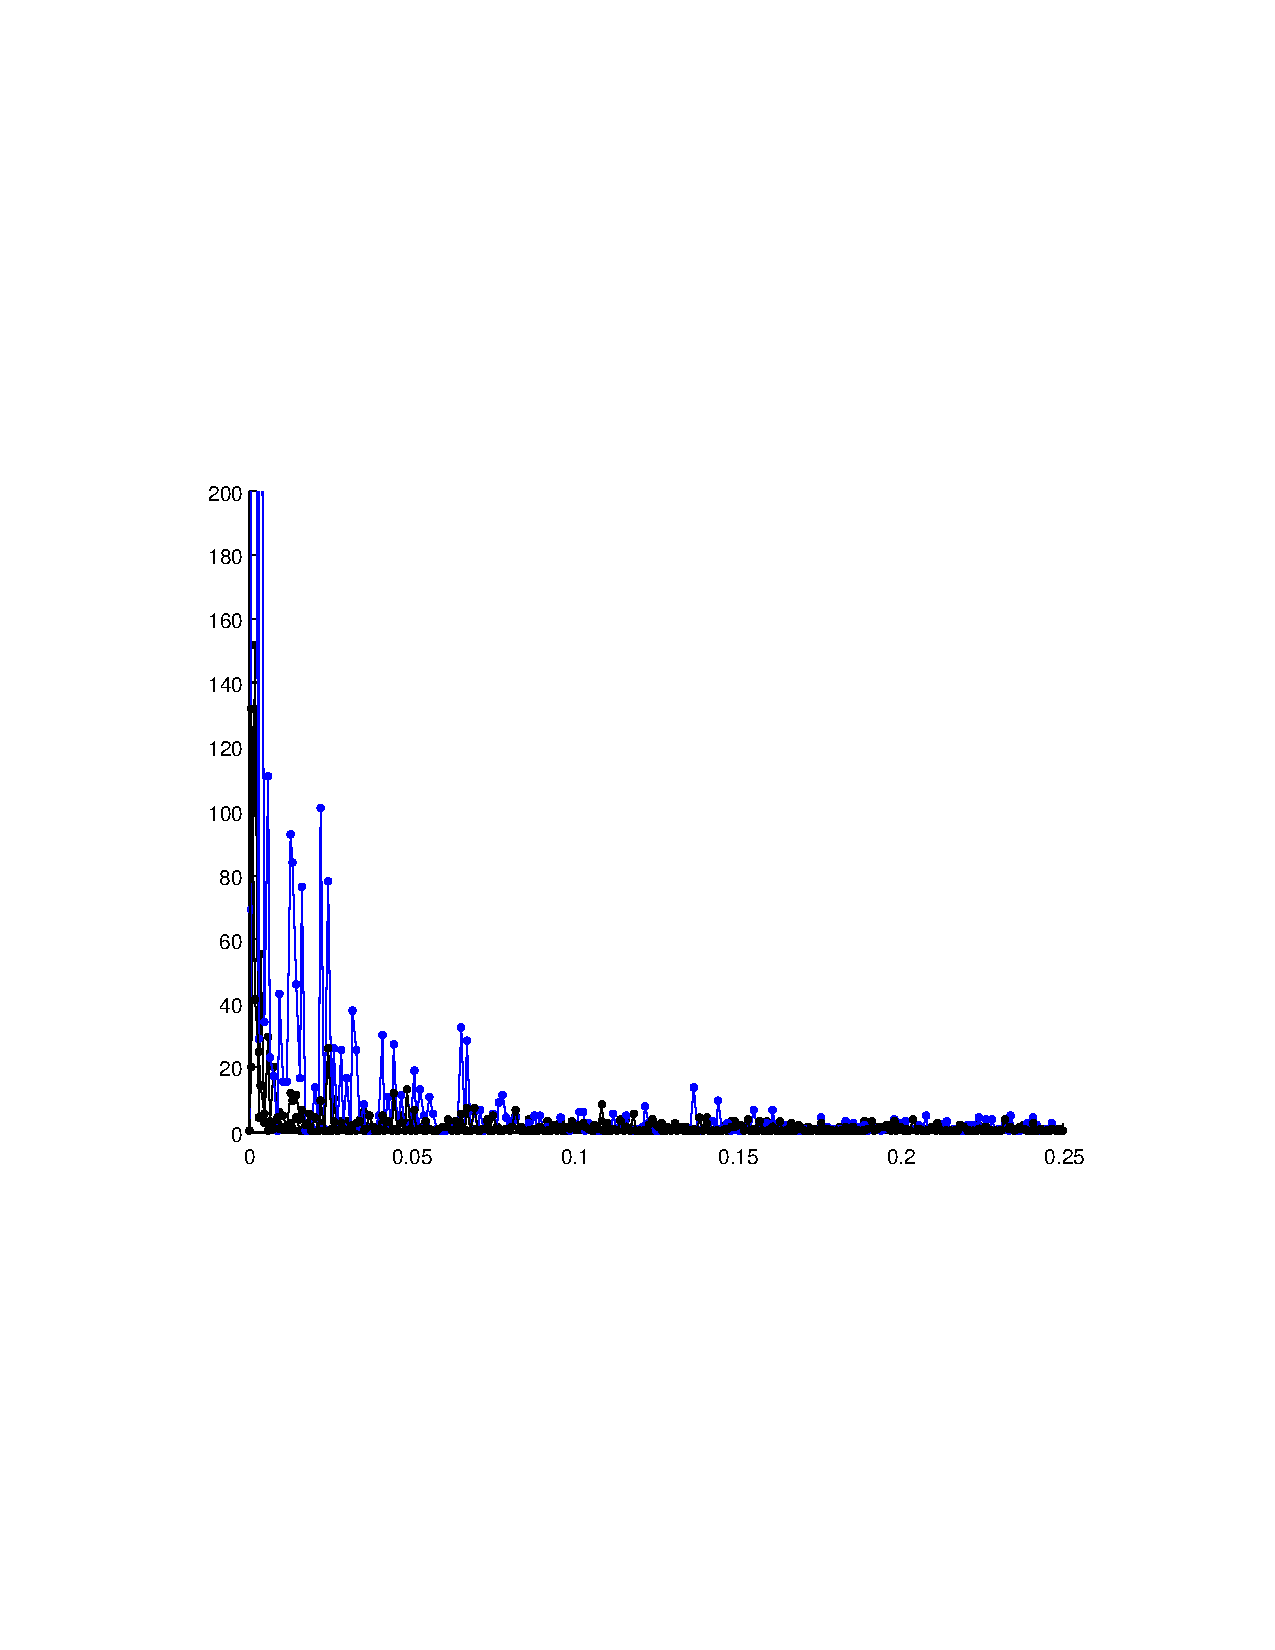
\includegraphics[width = 0.24\textwidth]{figures2/freq_before_3}
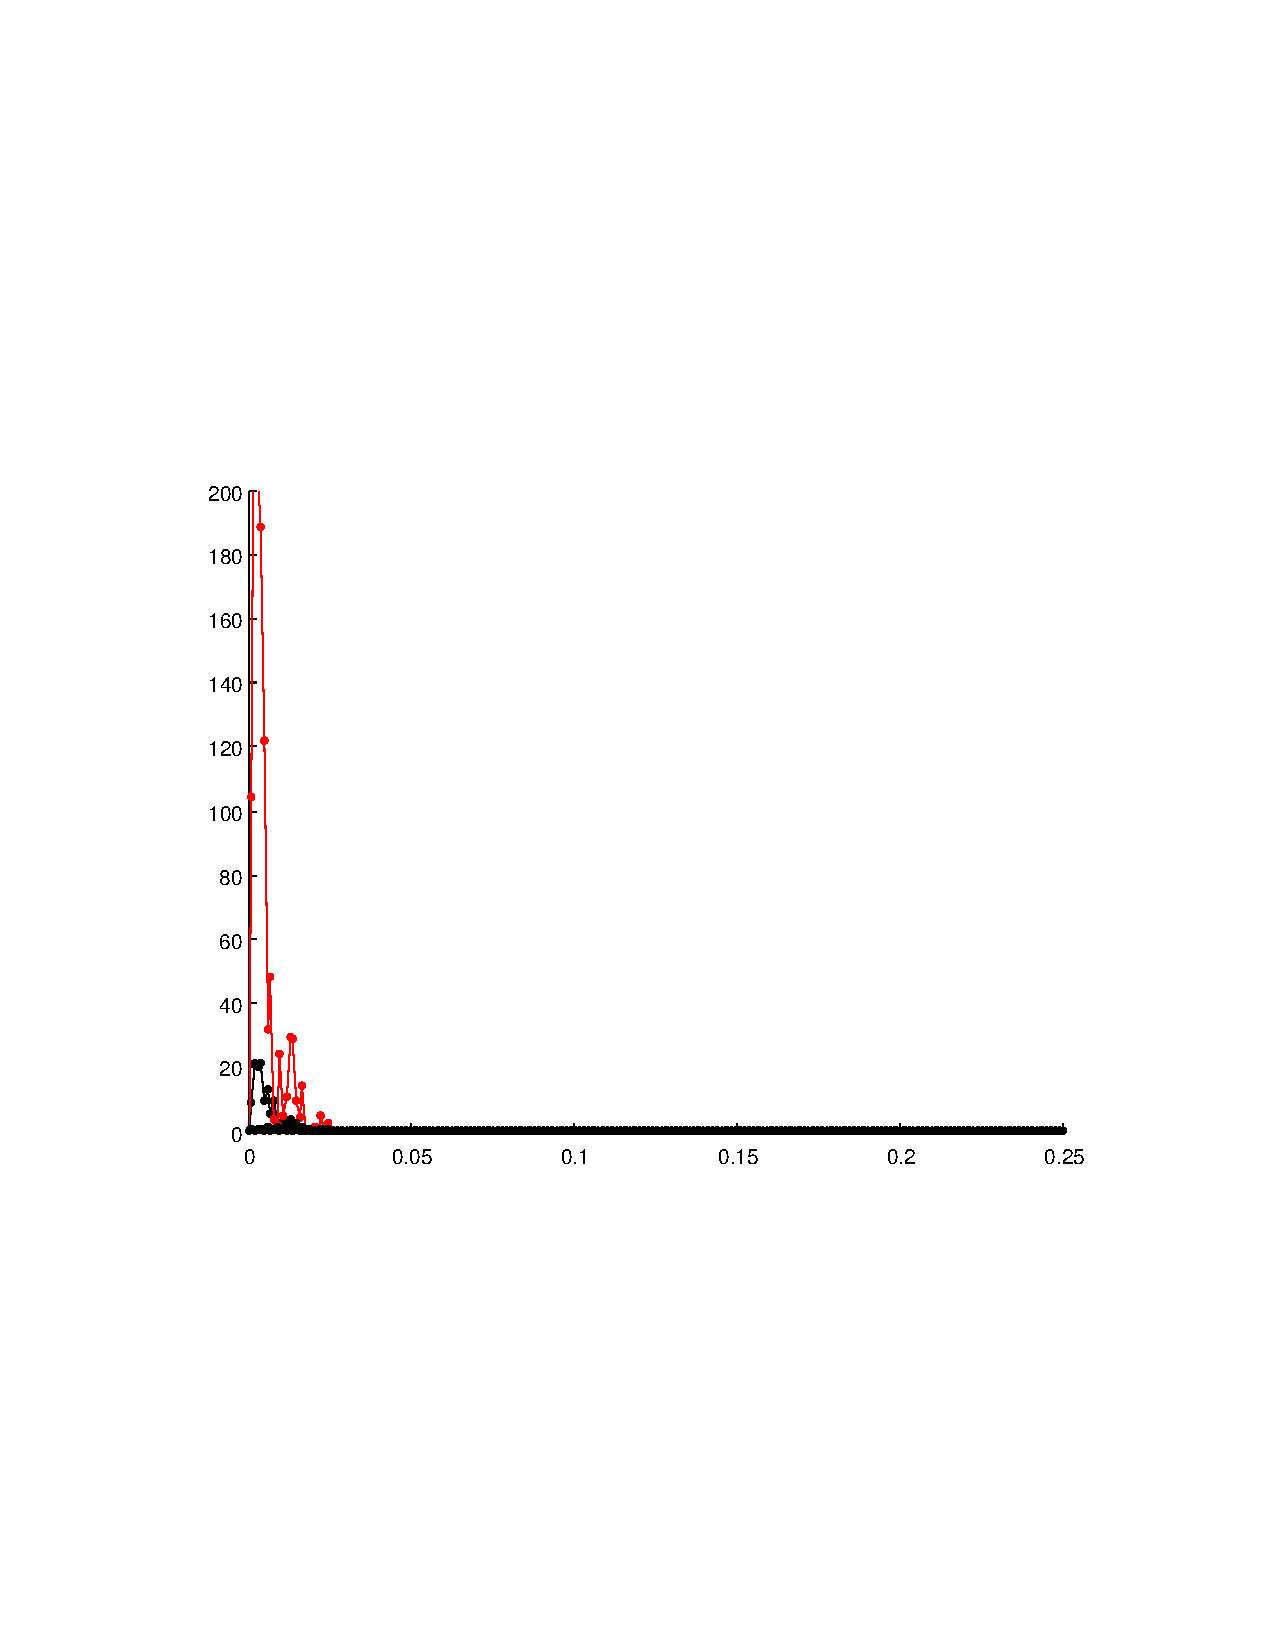
\includegraphics[width = 0.24\textwidth]{figures2/freq_after_3} \\
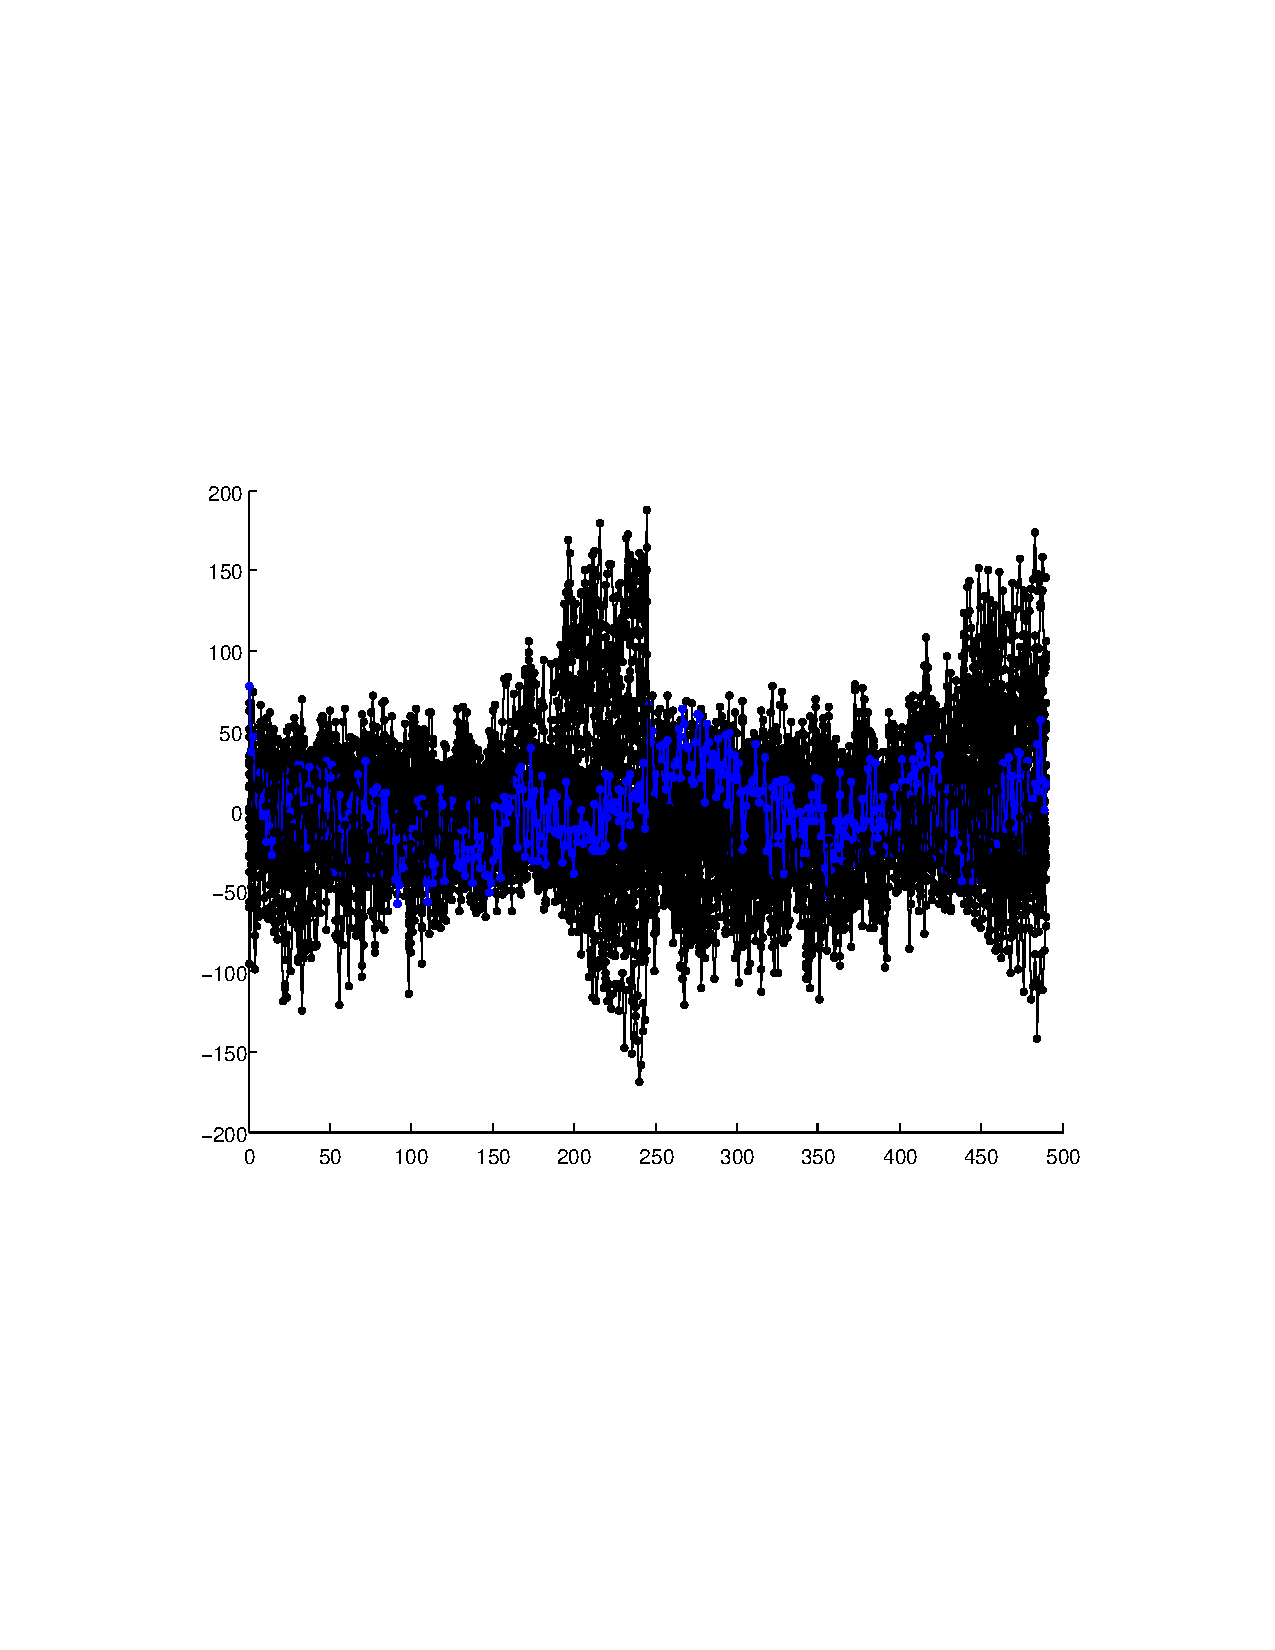
\includegraphics[width = 0.24\textwidth]{figures2/ts_before_25}
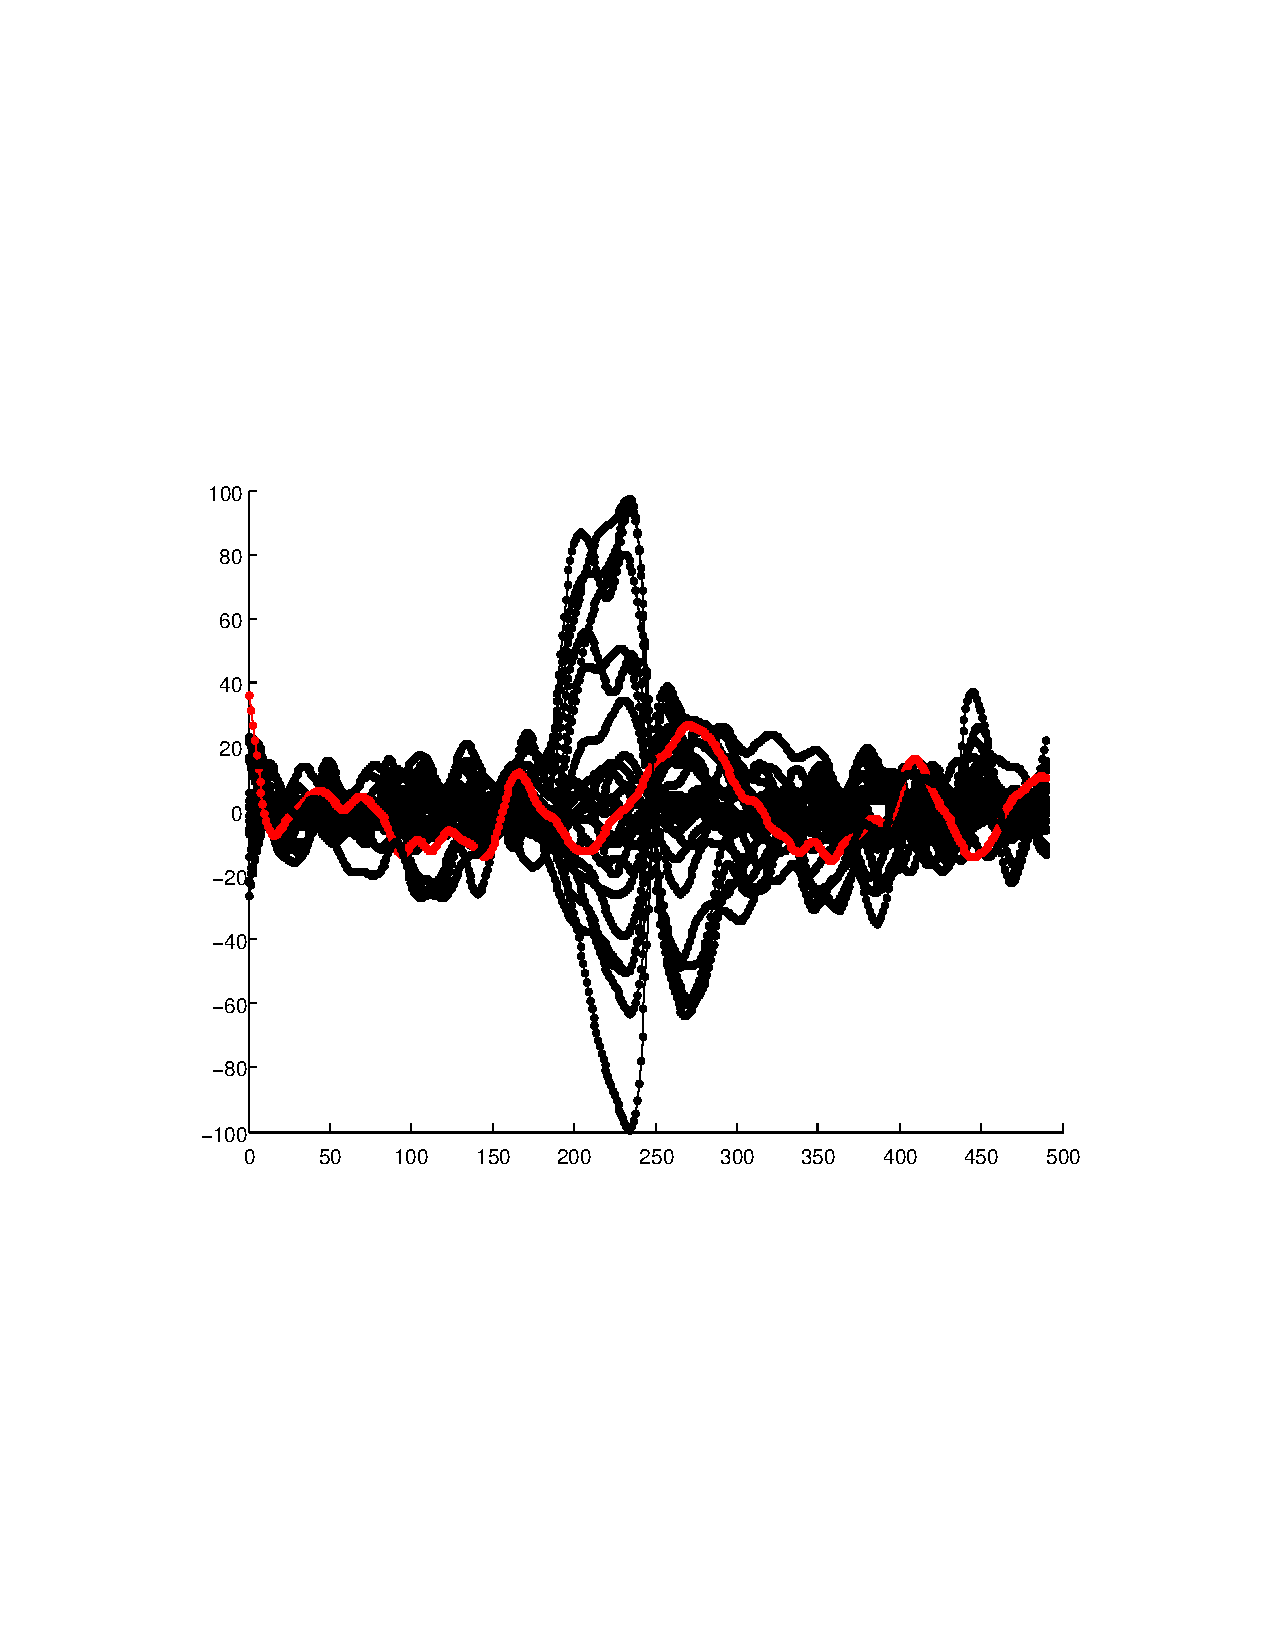
\includegraphics[width = 0.24\textwidth]{figures2/ts_after_25}
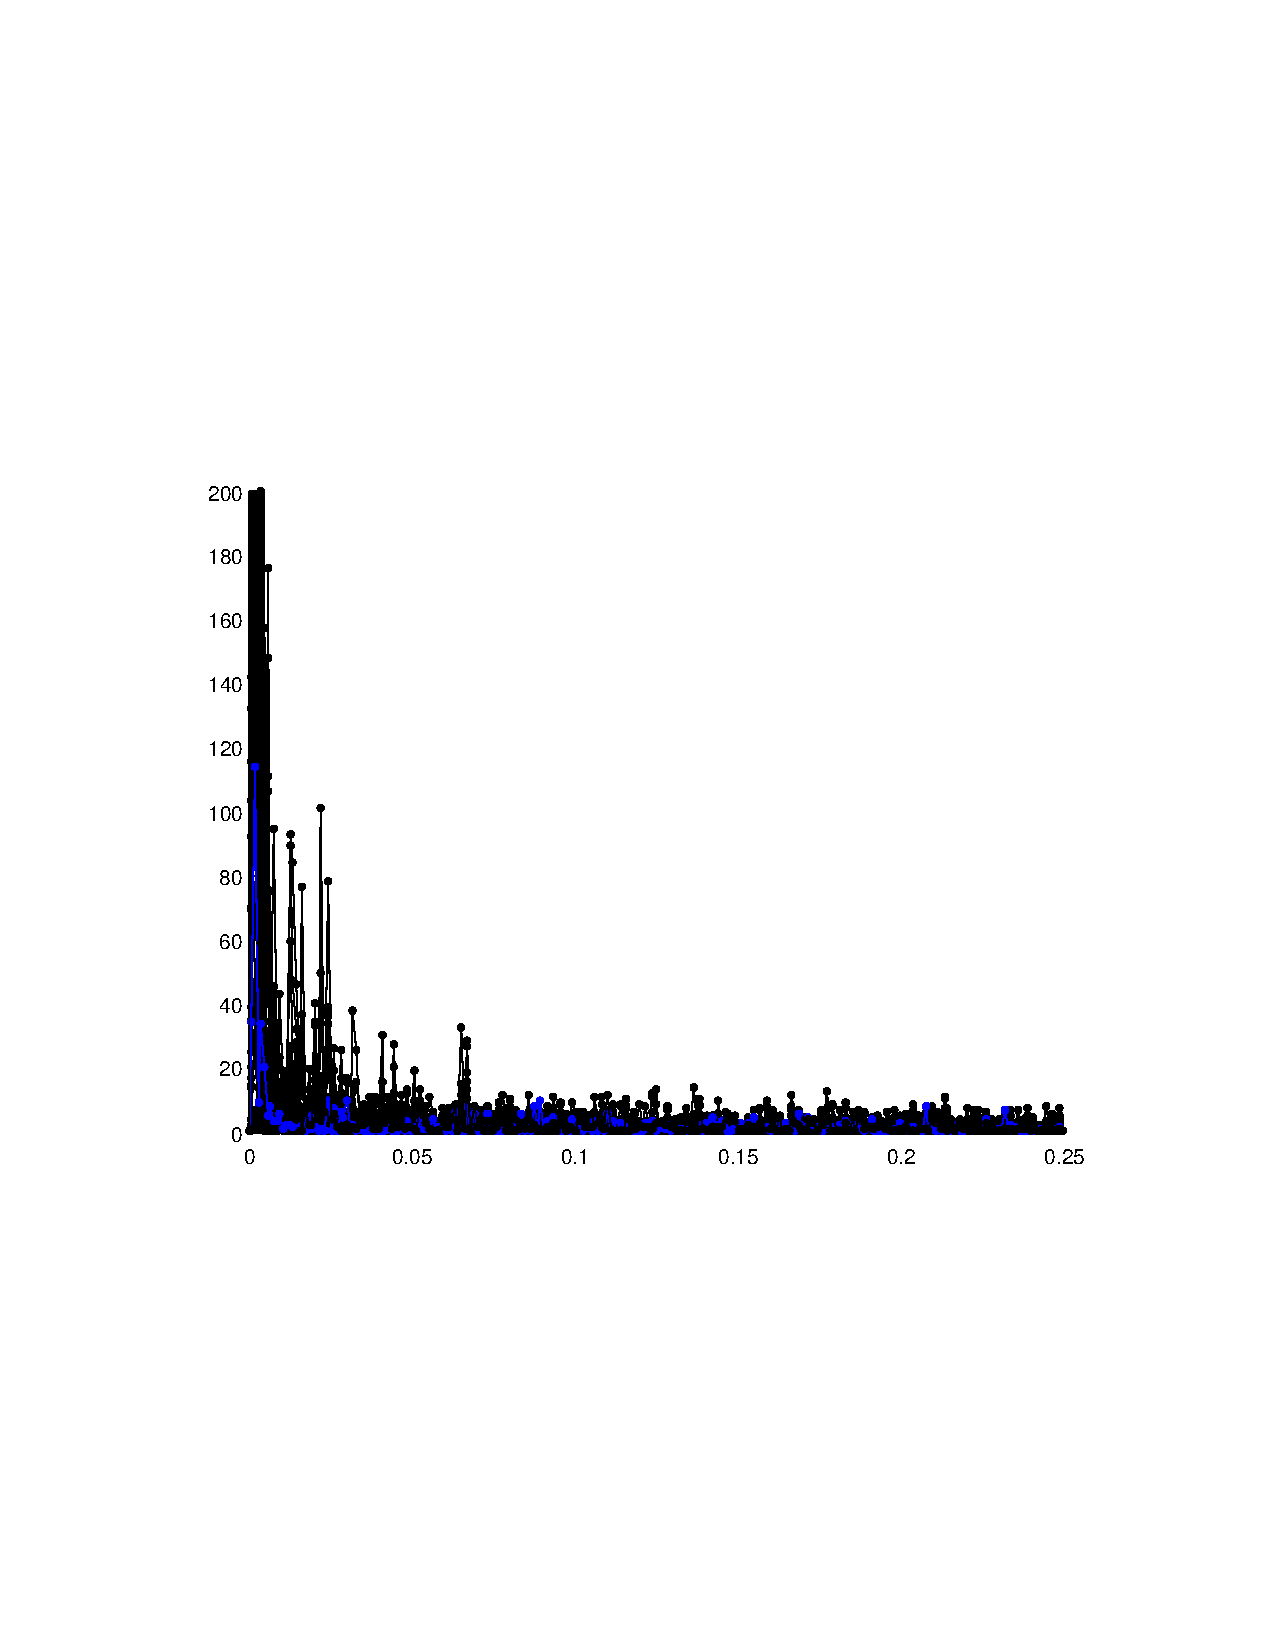
\includegraphics[width = 0.24\textwidth]{figures2/freq_before_25}
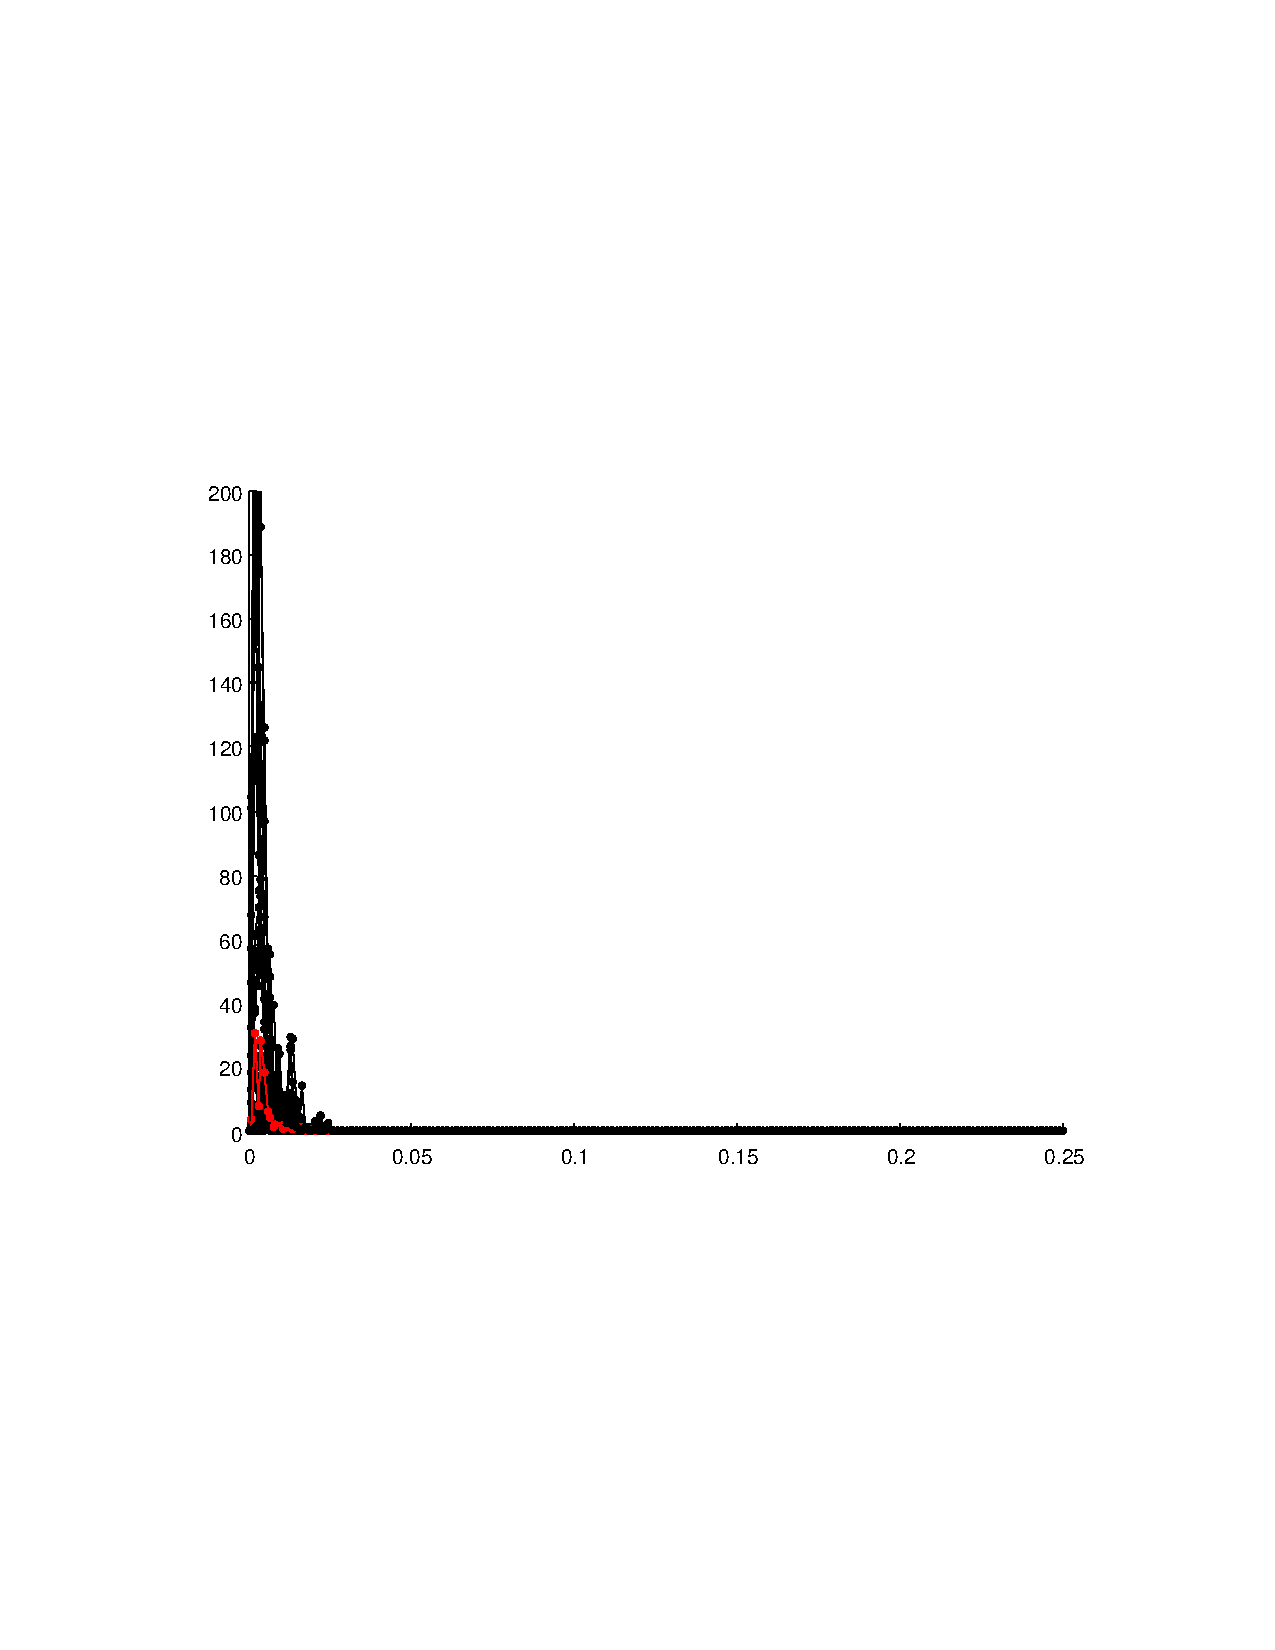
\includegraphics[width = 0.24\textwidth]{figures2/freq_after_25} \\
\caption{Time sequence before and after bandpass filtering. each row is a time course.}
\label{fig104}
\end{figure}

\begin{figure}[htb]
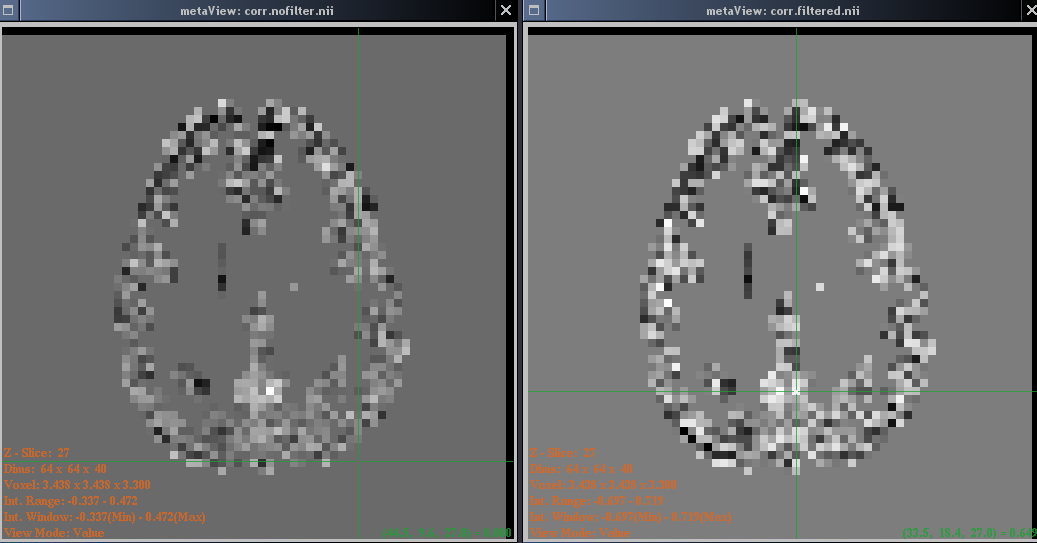
\includegraphics[width = 1\textwidth]{figures2/corrmap_both}\\
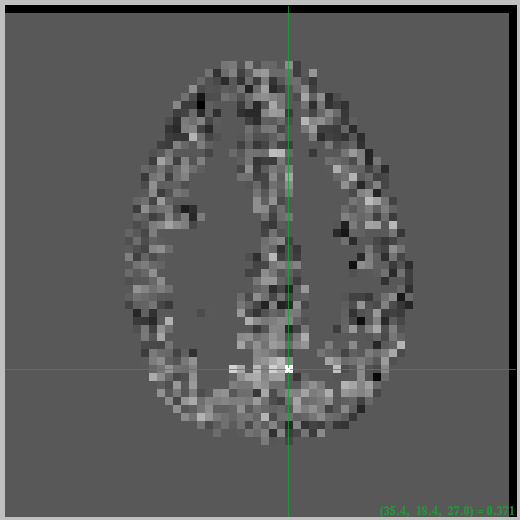
\includegraphics[width = 0.48\textwidth]{figures2/corrmap_nofilter_R2}
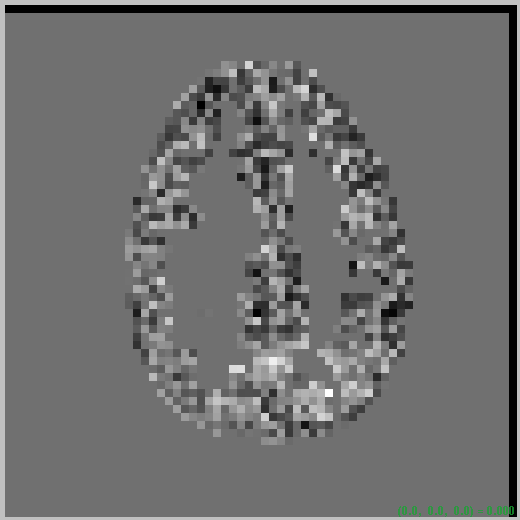
\includegraphics[width = 0.48\textwidth]{figures2/corrmap_filtered_R2}\\
\caption{correlation map. Left is before bandpass filtering, and right is after bandpass filtering. First row is dataset R1, second row is dataset R2. Seed voxel is [34 28 27].}
\label{fig105}
\end{figure}

\section{May 25}
\textbf{Standard SPM method: } In Greicius paper, a ROI is selected as a covariate (regressor), and linear regression (SPM) method is used to get the contrast map of whole brain. The linear regression parameter $\hat \beta$ is not equivalent to the sample correlation between regressor time sequence and other time sequence. To see that sample correlation $r_{xy} = \sum_i x_i y_i /(N-1) s_x s_y$. But in linear regression $\mat Y = \mat X \beta + \varepsilon$, the estimator of $\beta$ is $\hat \beta = \sum_i x_i y_i / \sum_i x_i^2$, and we see $\hat \beta = (s_y/s_x) r_{xy}$. That means, even if two voxels have small correlation, the linear regression parameter $\beta$ may be large. 

When we divide $x$ and $y$ by their standard deviation $s_x$ and $s_y$, $\hat \beta $ will be equal to sample correlation $r_{xy}$. So, linear regression in this case is amount to compute sample correlation btween two data points on a sphere.

\begin{itemize}
\item Preprocessing: motion correction by SPM.
\item Spatial smoothing by SPM. 
\item Use \textsf{fslmaths} to convert to float type. \texttt{ fslmaths srfmri.nii -add 0 srfmri\_f.nii -odt float}
\item Temporal filtering by FSL. \texttt{fslmaths srfmri  -bptf 55 6 fsrfmri}
\item Choose seed voxel, get regressor by averaging around seed voxel. 
\item Linear regression, and estimate coefficients $\beta$ for the whole volume.
\item Also compute correlation between seed regressor and all other voxels.
\end{itemize}

\section{Jun 9}
Use \textsf{conn} for functional connectivity analysis. Processing: motion correction, slice timing, registration with T1 an T2, normalization, spatial smoothing. I found (1). Adding motion parameters as confounds improve the results a little? (2) more PCA components and derivatives of covariates improves results. (3) Spatial smoothing makes a big difference. 

\section{Jun 16}
\begin{figure}
\includegraphics[width = 0.4\textwidth]{figures2/wraf}
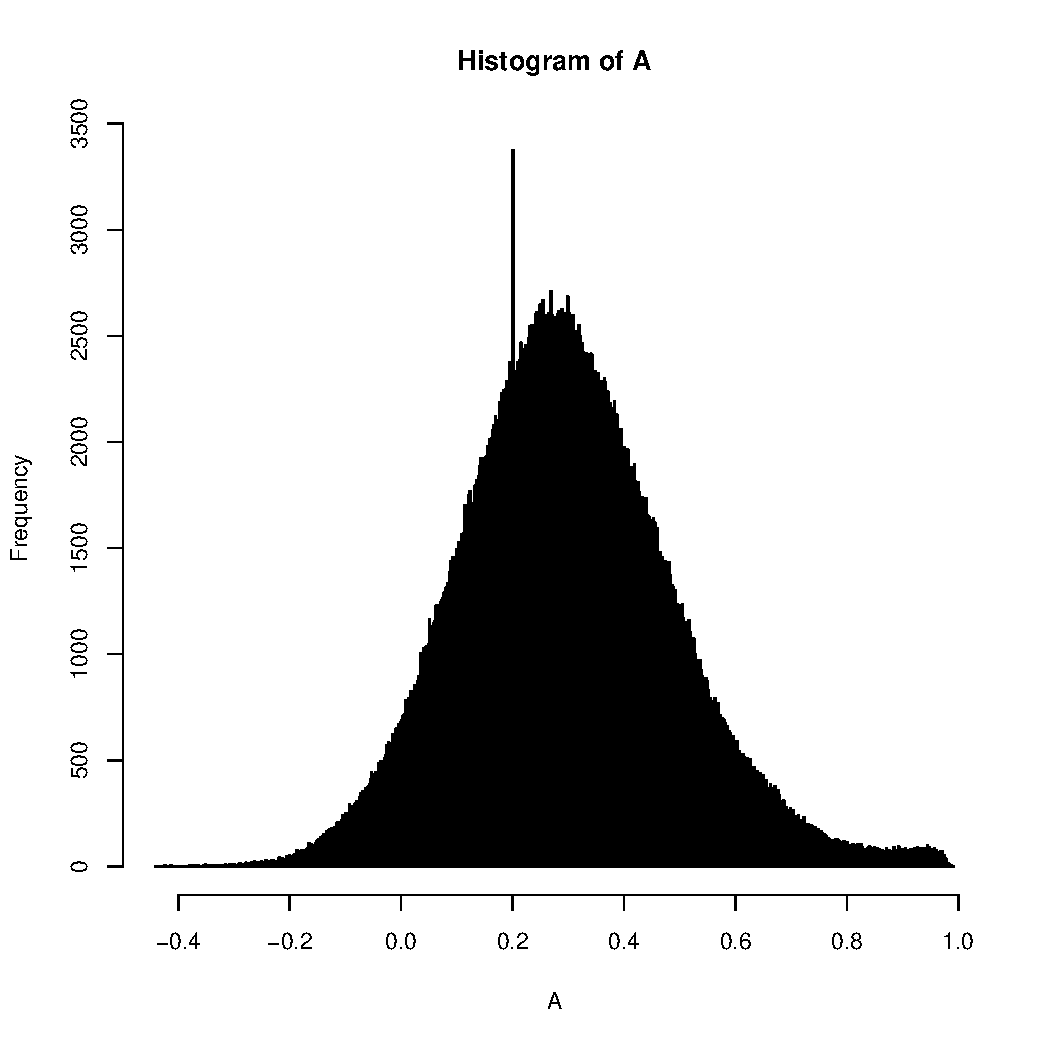
\includegraphics[width = 0.4\textwidth]{figures2/swarf}\\
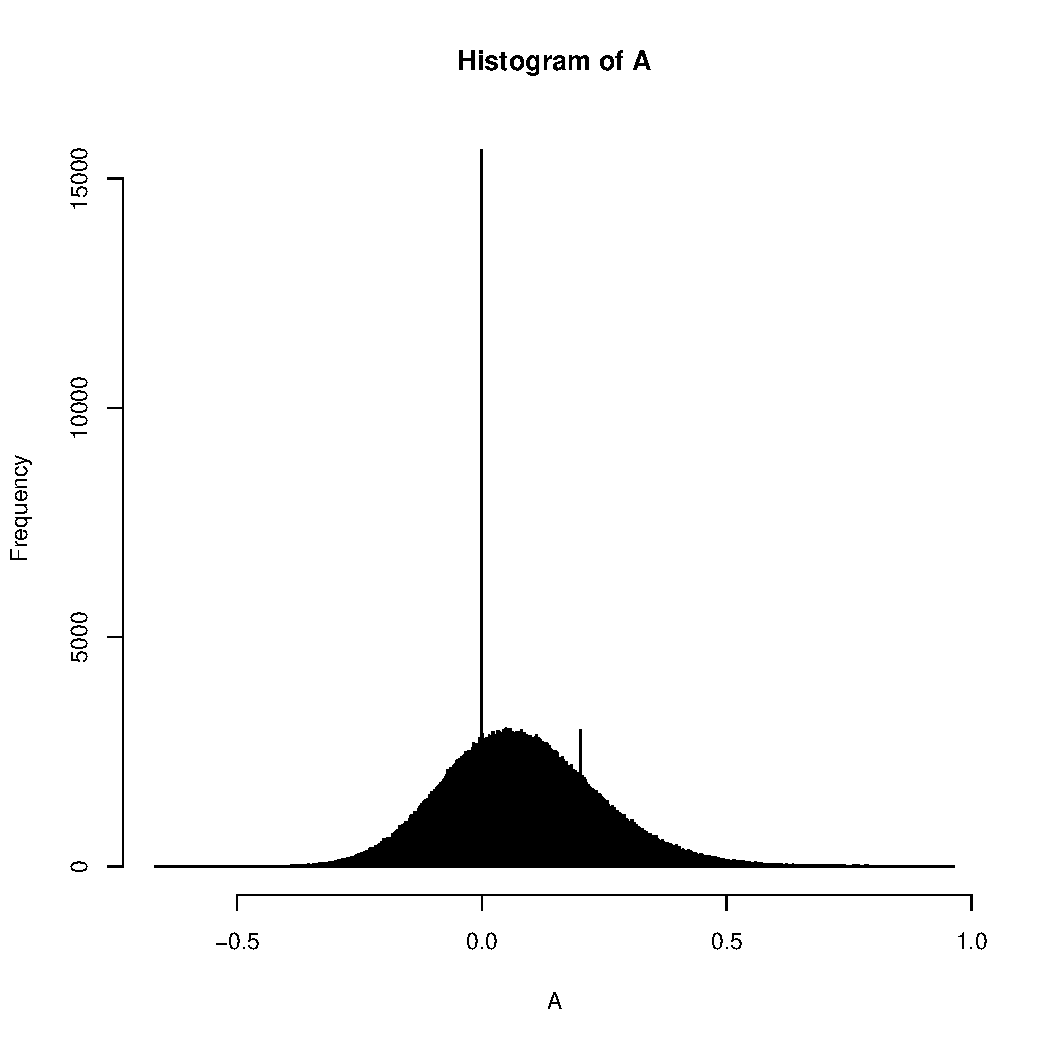
\includegraphics[width = 0.4\textwidth]{figures2/3mm_preprocessed}
\end{figure}

\section{Junn 22}
By tuning $\alpha$ term in MRF's clique potential function, we can choose the relative proportion between the 'connected' cluster and 'un-connected' cluster. The $\alpha$ term is similar to the $p$ value in standard SPM method. 

By tuning $\beta$ term in MRF's clique potential function we can choose how the connectivity map is partitioned into (i.e. big chunks or small chunks). The $\beta$ term is similar to the spatial smoothing kernel size in SPM.

So what's the sense of our MRF since what $\alpha$ and $\beta$ can do are also can be done by spatial smoothing. The answer is MRF give a concept of neighborhood. And by re-defining neighborhood, we can incorporate inter-subject information, or multi-modality information (DTI) into this neighborhood system. 

\textbf{Summary of talk with Tom: } For group analysis, we need $p(X | D_1, D_2,\dots) = p(D_1,\dots, | X) \cdot p(X) = p(D_1|X)\cdot p(D_2|X) \cdot p(D_3|X)$. 

\section{June 28: Review of ICA}
for Gaussian distribution, uncorrelatedneww and independence become the same thing.

For PCA, we can derive the projection matrix without knowing the data distribution. PGA does not use data distribution either? But for ICA, one of the two assumptions is non-Gaussian, which is related to the data distribution. How to add this information in Riemannian Geometry? 

Consider probalistic PCA. If we can generalize PPCA into Riemannian space, we may also generalize ICA. This is because PPCA has distribution information in it, and is more similar to PCA.

\section{Aug 19 fMRI clustering review}
 


\section{Scratch Pad}
spontaneous brain activity. Spontaneous neuronal activity consume 20\% of total energy while task related only take 5\%.

One strategy to account for these non-neuronal noise is high sampling rate, which prevents aliasing of higher frequency of cardiac or respiratory activity. But this reduce spatial coverage.

Regions that have similar functionality in task paradigms, tends to be correlated in spontaneous activity.

Resting-state activity serves as a priori hypothesis that brain response to task conditions.

Temporal properties: 1/f. Only frequency below 0.1 Hz is good. (do we need a low pass filter?)

The spontaneous activity can increase SNR of task by correcting. Maybe it explains many inter-trail variability. 

The decrease/deactivation arise from unrecognized increases/activations? No enough information of the control state to judge this.

real data --> \textit{in vivo} data

red blood cell carry hemoglobin (xuehongsu), which store oxygen molecule. hemoglobin can release and absorb oxygen. At lungs, red blood contain hemoglobin, which is oxygenated, then deoxygenated. Oxygenated and de-oxygenated hemoglobin have different magnetic properties: 

If we just use band-pass filter before calculating correlation, is there any difference with frequency method, i.e., spectral coherence averaging at different frequency point.

Is there any need for slice-timing correction. In SPM, they do not recommend to do it because there is probably a regressor(1st derivative of HRF) that can take care of slice timing issue. But for resting state connectivity we do not have such feature. Furthermore, for inter-leaved EPI sequence, there is even more need for this.(mindhive.mit.edu/node/109)

Global normalization. Remove the difference between volumes in different time point??? search spm manual for 'global normalization'.

3/25: Found high pass filter make the detection worse. (high pass filter sigma = 20 TR). Also found low pass filter make detection worse, though it's slightly better than applying high pass filter. (low pass sigma = 2 TR).

\bibliographystyle{plainnat}
\bibliography{/home/sci/weiliu/projects/zotero}
\end{document}
 
